\documentclass[twoside]{book}

% Packages required by doxygen
\usepackage{fixltx2e}
\usepackage{calc}
\usepackage{doxygen}
\usepackage[export]{adjustbox} % also loads graphicx
\usepackage{graphicx}
\usepackage[utf8]{inputenc}
\usepackage{makeidx}
\usepackage{multicol}
\usepackage{multirow}
\PassOptionsToPackage{warn}{textcomp}
\usepackage{textcomp}
\usepackage[nointegrals]{wasysym}
\usepackage[table]{xcolor}

% NLS support packages
\usepackage[spanish]{babel}
% Font selection
\usepackage[T1]{fontenc}
\usepackage[scaled=.90]{helvet}
\usepackage{courier}
\usepackage{amssymb}
\usepackage{sectsty}
\renewcommand{\familydefault}{\sfdefault}
\allsectionsfont{%
  \fontseries{bc}\selectfont%
  \color{darkgray}%
}
\renewcommand{\DoxyLabelFont}{%
  \fontseries{bc}\selectfont%
  \color{darkgray}%
}
\newcommand{\+}{\discretionary{\mbox{\scriptsize$\hookleftarrow$}}{}{}}

% Page & text layout
\usepackage{geometry}
\geometry{%
  a4paper,%
  top=2.5cm,%
  bottom=2.5cm,%
  left=2.5cm,%
  right=2.5cm%
}
\tolerance=750
\hfuzz=15pt
\hbadness=750
\setlength{\emergencystretch}{15pt}
\setlength{\parindent}{0cm}
\setlength{\parskip}{3ex plus 2ex minus 2ex}
\makeatletter
\renewcommand{\paragraph}{%
  \@startsection{paragraph}{4}{0ex}{-1.0ex}{1.0ex}{%
    \normalfont\normalsize\bfseries\SS@parafont%
  }%
}
\renewcommand{\subparagraph}{%
  \@startsection{subparagraph}{5}{0ex}{-1.0ex}{1.0ex}{%
    \normalfont\normalsize\bfseries\SS@subparafont%
  }%
}
\makeatother

% Headers & footers
\usepackage{fancyhdr}
\pagestyle{fancyplain}
\fancyhead[LE]{\fancyplain{}{\bfseries\thepage}}
\fancyhead[CE]{\fancyplain{}{}}
\fancyhead[RE]{\fancyplain{}{\bfseries\leftmark}}
\fancyhead[LO]{\fancyplain{}{\bfseries\rightmark}}
\fancyhead[CO]{\fancyplain{}{}}
\fancyhead[RO]{\fancyplain{}{\bfseries\thepage}}
\fancyfoot[LE]{\fancyplain{}{}}
\fancyfoot[CE]{\fancyplain{}{}}
\fancyfoot[RE]{\fancyplain{}{\bfseries\scriptsize Generado por Doxygen }}
\fancyfoot[LO]{\fancyplain{}{\bfseries\scriptsize Generado por Doxygen }}
\fancyfoot[CO]{\fancyplain{}{}}
\fancyfoot[RO]{\fancyplain{}{}}
\renewcommand{\footrulewidth}{0.4pt}
\renewcommand{\chaptermark}[1]{%
  \markboth{#1}{}%
}
\renewcommand{\sectionmark}[1]{%
  \markright{\thesection\ #1}%
}

% Indices & bibliography
\usepackage{natbib}
\usepackage[titles]{tocloft}
\setcounter{tocdepth}{3}
\setcounter{secnumdepth}{5}
\makeindex

% Hyperlinks (required, but should be loaded last)
\usepackage{ifpdf}
\ifpdf
  \usepackage[pdftex,pagebackref=true]{hyperref}
\else
  \usepackage[ps2pdf,pagebackref=true]{hyperref}
\fi
\hypersetup{%
  colorlinks=true,%
  linkcolor=blue,%
  citecolor=blue,%
  unicode%
}

% Custom commands
\newcommand{\clearemptydoublepage}{%
  \newpage{\pagestyle{empty}\cleardoublepage}%
}

\usepackage{caption}
\captionsetup{labelsep=space,justification=centering,font={bf},singlelinecheck=off,skip=4pt,position=top}

%===== C O N T E N T S =====

\begin{document}

% Titlepage & ToC
\hypersetup{pageanchor=false,
             bookmarksnumbered=true,
             pdfencoding=unicode
            }
\pagenumbering{alph}
\begin{titlepage}
\vspace*{7cm}
\begin{center}%
{\Large E\+V\+A\+L\+U\+A\+T\+OR\+: plataforma de gestión de problemas y cursos de programación \\[1ex]\large version 2.\+0 17-\/may-\/2021 }\\
\vspace*{1cm}
{\large Generado por Doxygen 1.8.14}\\
\end{center}
\end{titlepage}
\clearemptydoublepage
\pagenumbering{roman}
\tableofcontents
\clearemptydoublepage
\pagenumbering{arabic}
\hypersetup{pageanchor=true}

%--- Begin generated contents ---
\chapter{Página principal}
\label{index}\hypertarget{index}{}E\+V\+A\+L\+U\+A\+T\+OR\+: plataforma de gestión de problemas y cursos de programación.

Programa modular para la gestion de la plataforma E\+V\+A\+L\+U\+A\+T\+OR, una plataforma de gestión de problemas y cursos de programación. Está formado por las clases {\itshape \mbox{\hyperlink{class_cjt__cursos}{Cjt\+\_\+cursos}}}, {\itshape \mbox{\hyperlink{class_cjt__problemas}{Cjt\+\_\+problemas}}}, {\itshape \mbox{\hyperlink{class_cjt__sesiones}{Cjt\+\_\+sesiones}}}, {\itshape \mbox{\hyperlink{class_cjt__usuarios}{Cjt\+\_\+usuarios}}}, {\itshape \mbox{\hyperlink{class_curso}{Curso}}}, {\itshape \mbox{\hyperlink{class_problema}{Problema}}}, {\itshape \mbox{\hyperlink{class_sesion}{Sesion}}} y {\itshape \mbox{\hyperlink{class_usuario}{Usuario}}}.

El programa principal se encuentra en el módulo {\itshape main.\+cc} 
\chapter{Índice de clases}
\section{Lista de clases}
Lista de las clases, estructuras, uniones e interfaces con una breve descripción\+:\begin{DoxyCompactList}
\item\contentsline{section}{\mbox{\hyperlink{class_cjt__cursos}{Cjt\+\_\+cursos}} \\*Representa un \mbox{\hyperlink{class_cjt__cursos}{Cjt\+\_\+cursos}} (conjunto de cursos) }{\pageref{class_cjt__cursos}}{}
\item\contentsline{section}{\mbox{\hyperlink{class_cjt__problemas}{Cjt\+\_\+problemas}} \\*Representa un \mbox{\hyperlink{class_cjt__problemas}{Cjt\+\_\+problemas}} (conjunto de problemas) }{\pageref{class_cjt__problemas}}{}
\item\contentsline{section}{\mbox{\hyperlink{class_cjt__sesiones}{Cjt\+\_\+sesiones}} \\*Representa un \mbox{\hyperlink{class_cjt__sesiones}{Cjt\+\_\+sesiones}} (conjunto de sesiones) }{\pageref{class_cjt__sesiones}}{}
\item\contentsline{section}{\mbox{\hyperlink{class_cjt__usuarios}{Cjt\+\_\+usuarios}} \\*Representa un \mbox{\hyperlink{class_cjt__usuarios}{Cjt\+\_\+usuarios}} (conjunto de usuarios) }{\pageref{class_cjt__usuarios}}{}
\item\contentsline{section}{\mbox{\hyperlink{class_curso}{Curso}} \\*Representa un \mbox{\hyperlink{class_curso}{Curso}} de la plataforma }{\pageref{class_curso}}{}
\item\contentsline{section}{\mbox{\hyperlink{struct_cjt__problemas_1_1prat}{Cjt\+\_\+problemas\+::prat}} }{\pageref{struct_cjt__problemas_1_1prat}}{}
\item\contentsline{section}{\mbox{\hyperlink{class_problema}{Problema}} \\*Representa un \mbox{\hyperlink{class_problema}{Problema}} de una \mbox{\hyperlink{class_sesion}{Sesion}} de la plataforma }{\pageref{class_problema}}{}
\item\contentsline{section}{\mbox{\hyperlink{class_sesion}{Sesion}} \\*Representa una \mbox{\hyperlink{class_sesion}{Sesion}} de la plataforma }{\pageref{class_sesion}}{}
\item\contentsline{section}{\mbox{\hyperlink{class_usuario}{Usuario}} \\*Representa un \mbox{\hyperlink{class_usuario}{Usuario}} registrado en la plataforma }{\pageref{class_usuario}}{}
\end{DoxyCompactList}

\chapter{Indice de archivos}
\section{Lista de archivos}
Lista de todos los archivos con descripciones breves\+:\begin{DoxyCompactList}
\item\contentsline{section}{\mbox{\hyperlink{_cjt__cursos_8cc}{Cjt\+\_\+cursos.\+cc}} }{\pageref{_cjt__cursos_8cc}}{}
\item\contentsline{section}{\mbox{\hyperlink{_cjt__cursos_8hh}{Cjt\+\_\+cursos.\+hh}} \\*Especificación de la clase \mbox{\hyperlink{class_cjt__cursos}{Cjt\+\_\+cursos}} (conjunto de cursos) }{\pageref{_cjt__cursos_8hh}}{}
\item\contentsline{section}{\mbox{\hyperlink{_cjt__problemas_8cc}{Cjt\+\_\+problemas.\+cc}} }{\pageref{_cjt__problemas_8cc}}{}
\item\contentsline{section}{\mbox{\hyperlink{_cjt__problemas_8hh}{Cjt\+\_\+problemas.\+hh}} \\*Especificación de la clase \mbox{\hyperlink{class_cjt__problemas}{Cjt\+\_\+problemas}} (conjunto de problemas) }{\pageref{_cjt__problemas_8hh}}{}
\item\contentsline{section}{\mbox{\hyperlink{_cjt__sesiones_8cc}{Cjt\+\_\+sesiones.\+cc}} }{\pageref{_cjt__sesiones_8cc}}{}
\item\contentsline{section}{\mbox{\hyperlink{_cjt__sesiones_8hh}{Cjt\+\_\+sesiones.\+hh}} \\*Especificación de la clase conjunto de sesiones }{\pageref{_cjt__sesiones_8hh}}{}
\item\contentsline{section}{\mbox{\hyperlink{_cjt__usuarios_8cc}{Cjt\+\_\+usuarios.\+cc}} }{\pageref{_cjt__usuarios_8cc}}{}
\item\contentsline{section}{\mbox{\hyperlink{_cjt__usuarios_8hh}{Cjt\+\_\+usuarios.\+hh}} \\*Especificación de la clase \mbox{\hyperlink{class_cjt__usuarios}{Cjt\+\_\+usuarios}} (conjunto de usuarios) }{\pageref{_cjt__usuarios_8hh}}{}
\item\contentsline{section}{\mbox{\hyperlink{_curso_8cc}{Curso.\+cc}} }{\pageref{_curso_8cc}}{}
\item\contentsline{section}{\mbox{\hyperlink{_curso_8hh}{Curso.\+hh}} \\*Especificación de la clase \mbox{\hyperlink{class_curso}{Curso}} }{\pageref{_curso_8hh}}{}
\item\contentsline{section}{\mbox{\hyperlink{_problema_8cc}{Problema.\+cc}} }{\pageref{_problema_8cc}}{}
\item\contentsline{section}{\mbox{\hyperlink{_problema_8hh}{Problema.\+hh}} \\*Especificación de la clase \mbox{\hyperlink{class_problema}{Problema}} }{\pageref{_problema_8hh}}{}
\item\contentsline{section}{\mbox{\hyperlink{program_8cc}{program.\+cc}} }{\pageref{program_8cc}}{}
\item\contentsline{section}{\mbox{\hyperlink{_sesion_8cc}{Sesion.\+cc}} }{\pageref{_sesion_8cc}}{}
\item\contentsline{section}{\mbox{\hyperlink{_sesion_8hh}{Sesion.\+hh}} \\*Especificación de la clase sesion }{\pageref{_sesion_8hh}}{}
\item\contentsline{section}{\mbox{\hyperlink{_usuario_8cc}{Usuario.\+cc}} }{\pageref{_usuario_8cc}}{}
\item\contentsline{section}{\mbox{\hyperlink{_usuario_8hh}{Usuario.\+hh}} \\*Especificación de la clase usuario }{\pageref{_usuario_8hh}}{}
\end{DoxyCompactList}

\chapter{Documentación de las clases}
\hypertarget{class_cjt__cursos}{}\section{Referencia de la Clase Cjt\+\_\+cursos}
\label{class_cjt__cursos}\index{Cjt\+\_\+cursos@{Cjt\+\_\+cursos}}


Representa un \mbox{\hyperlink{class_cjt__cursos}{Cjt\+\_\+cursos}} (conjunto de cursos)  


\subsection*{Métodos públicos}
\begin{DoxyCompactItemize}
\item 
\mbox{\hyperlink{class_cjt__cursos_acabe06047f0b2a3093dc75c8a70a4dd2}{Cjt\+\_\+cursos}} ()
\begin{DoxyCompactList}\small\item\em Creadora por defecto. \end{DoxyCompactList}\item 
void \mbox{\hyperlink{class_cjt__cursos_ae2e0a96f014dda94b0d8465838cf14b6}{nuevo\+\_\+curso}} (\mbox{\hyperlink{class_cjt__sesiones}{Cjt\+\_\+sesiones}} \&sesiones)
\begin{DoxyCompactList}\small\item\em Añade un curso en un \mbox{\hyperlink{class_cjt__cursos}{Cjt\+\_\+cursos}}. \end{DoxyCompactList}\item 
void \mbox{\hyperlink{class_cjt__cursos_a974c8ac07471f9354fb13616a489f726}{alta}} (int c)
\begin{DoxyCompactList}\small\item\em Augmenta en una unidad el nº de inscritos en un curso c de un \mbox{\hyperlink{class_cjt__cursos}{Cjt\+\_\+cursos}}. \end{DoxyCompactList}\item 
void \mbox{\hyperlink{class_cjt__cursos_a01b47ced7b3b96ea87775bb4e2f0302a}{baja}} (int c)
\begin{DoxyCompactList}\small\item\em Disminuye en una unidad el nº de inscritos en un curso c de un \mbox{\hyperlink{class_cjt__cursos}{Cjt\+\_\+cursos}}. \end{DoxyCompactList}\item 
void \mbox{\hyperlink{class_cjt__cursos_a140c61d43f549aa71503f5b8b080c48c}{completado}} (int c)
\begin{DoxyCompactList}\small\item\em Augmenta en una unidad el nº de usuarios que han completado un curso. \end{DoxyCompactList}\item 
bool \mbox{\hyperlink{class_cjt__cursos_aed873ef8285d1f33c391bd4d808185de}{existe\+\_\+curso}} (int c) const
\begin{DoxyCompactList}\small\item\em Comprueba si existe un curso con identificador c en un \mbox{\hyperlink{class_cjt__cursos}{Cjt\+\_\+cursos}}. \end{DoxyCompactList}\item 
bool \mbox{\hyperlink{class_cjt__cursos_a7b2a3da42d49f10bd6413fa00dbe9012}{existe\+\_\+problema}} (const string \&p, int c) const
\begin{DoxyCompactList}\small\item\em Comprueba si existe un problema con identificador p en un curso c de un \mbox{\hyperlink{class_cjt__cursos}{Cjt\+\_\+cursos}}. \end{DoxyCompactList}\item 
string \mbox{\hyperlink{class_cjt__cursos_acbc9b738ae2d1ba8ba2633aa57561fcb}{id\+\_\+sesion}} (int c, int i) const
\begin{DoxyCompactList}\small\item\em Devuelve el identificador de una sesion en la posición i en la que se leyó en un curso c de un \mbox{\hyperlink{class_cjt__cursos}{Cjt\+\_\+cursos}}. \end{DoxyCompactList}\item 
int \mbox{\hyperlink{class_cjt__cursos_a3a8c9c5eecbdab5e1702233dab4d725b}{num\+\_\+sesiones}} (int c) const
\begin{DoxyCompactList}\small\item\em Devuelve el nº de sesiones de un curso c de un \mbox{\hyperlink{class_cjt__cursos}{Cjt\+\_\+cursos}}. \end{DoxyCompactList}\item 
void \mbox{\hyperlink{class_cjt__cursos_a71a9a083e2abceee34329462a804637a}{leer\+\_\+cursos}} (\mbox{\hyperlink{class_cjt__sesiones}{Cjt\+\_\+sesiones}} \&sesiones)
\begin{DoxyCompactList}\small\item\em Lee los cursos para un \mbox{\hyperlink{class_cjt__cursos}{Cjt\+\_\+cursos}} dado un nº de cursos a leer. \end{DoxyCompactList}\item 
string \mbox{\hyperlink{class_cjt__cursos_acc9074c9338d31947bdd84e3498580be}{sesion\+\_\+problema}} (int c, const string \&p) const
\begin{DoxyCompactList}\small\item\em Imprime el identificador de la sesion donde se realiza un problema p en un curso c de un \mbox{\hyperlink{class_cjt__cursos}{Cjt\+\_\+cursos}}. \end{DoxyCompactList}\item 
void \mbox{\hyperlink{class_cjt__cursos_a7d5981081ad5aeaa73bdd88b4a7f66c9}{imprimir\+\_\+num\+\_\+usuarios}} (int c) const
\begin{DoxyCompactList}\small\item\em Imprime el nº de usuarios inscritos en un curso c de un \mbox{\hyperlink{class_cjt__cursos}{Cjt\+\_\+cursos}}. \end{DoxyCompactList}\item 
void \mbox{\hyperlink{class_cjt__cursos_a6c98d2f0a31253b84dc8b4a0ea48c348}{escribir\+\_\+curso}} (int c) const
\begin{DoxyCompactList}\small\item\em Imprime un usuario con identificador c de un \mbox{\hyperlink{class_cjt__usuarios}{Cjt\+\_\+usuarios}}. \end{DoxyCompactList}\item 
void \mbox{\hyperlink{class_cjt__cursos_abba27f9593cae77bf02909a06454ec43}{listar\+\_\+cursos}} () const
\begin{DoxyCompactList}\small\item\em Lista los cursos actuales de la plataforma. \end{DoxyCompactList}\end{DoxyCompactItemize}
\subsection*{Atributos privados}
\begin{DoxyCompactItemize}
\item 
vector$<$ \mbox{\hyperlink{class_curso}{Curso}} $>$ \mbox{\hyperlink{class_cjt__cursos_a582f9540bc295212450dba4cd18c8886}{cursos}}
\end{DoxyCompactItemize}


\subsection{Descripción detallada}
Representa un \mbox{\hyperlink{class_cjt__cursos}{Cjt\+\_\+cursos}} (conjunto de cursos) 

Representa un conjunto de cursos. 

Definición en la línea 22 del archivo Cjt\+\_\+cursos.\+hh.



\subsection{Documentación del constructor y destructor}
\mbox{\Hypertarget{class_cjt__cursos_acabe06047f0b2a3093dc75c8a70a4dd2}\label{class_cjt__cursos_acabe06047f0b2a3093dc75c8a70a4dd2}} 
\index{Cjt\+\_\+cursos@{Cjt\+\_\+cursos}!Cjt\+\_\+cursos@{Cjt\+\_\+cursos}}
\index{Cjt\+\_\+cursos@{Cjt\+\_\+cursos}!Cjt\+\_\+cursos@{Cjt\+\_\+cursos}}
\subsubsection{\texorpdfstring{Cjt\+\_\+cursos()}{Cjt\_cursos()}}
{\footnotesize\ttfamily Cjt\+\_\+cursos\+::\+Cjt\+\_\+cursos (\begin{DoxyParamCaption}{ }\end{DoxyParamCaption})}



Creadora por defecto. 

\begin{DoxyPrecond}{Precondición}
cierto 
\end{DoxyPrecond}
\begin{DoxyPostcond}{Postcondición}
El resultado es un \mbox{\hyperlink{class_cjt__cursos}{Cjt\+\_\+cursos}} vacío 
\end{DoxyPostcond}


Definición en la línea 15 del archivo Cjt\+\_\+cursos.\+cc.


\begin{DoxyCode}
15 \{\}
\end{DoxyCode}


\subsection{Documentación de las funciones miembro}
\mbox{\Hypertarget{class_cjt__cursos_ae2e0a96f014dda94b0d8465838cf14b6}\label{class_cjt__cursos_ae2e0a96f014dda94b0d8465838cf14b6}} 
\index{Cjt\+\_\+cursos@{Cjt\+\_\+cursos}!nuevo\+\_\+curso@{nuevo\+\_\+curso}}
\index{nuevo\+\_\+curso@{nuevo\+\_\+curso}!Cjt\+\_\+cursos@{Cjt\+\_\+cursos}}
\subsubsection{\texorpdfstring{nuevo\+\_\+curso()}{nuevo\_curso()}}
{\footnotesize\ttfamily void Cjt\+\_\+cursos\+::nuevo\+\_\+curso (\begin{DoxyParamCaption}\item[{\mbox{\hyperlink{class_cjt__sesiones}{Cjt\+\_\+sesiones}} \&}]{sesiones }\end{DoxyParamCaption})}



Añade un curso en un \mbox{\hyperlink{class_cjt__cursos}{Cjt\+\_\+cursos}}. 

\begin{DoxyPrecond}{Precondición}
cierto 
\end{DoxyPrecond}
\begin{DoxyPostcond}{Postcondición}
El conjunto de cursos es el mismo con un nuevo curso más con el identificador N+1; si tiene problemas repetidos se imprime un mensaje de error y no se añade. En caso contrario, se imprime su identificador 
\end{DoxyPostcond}


Definición en la línea 25 del archivo Cjt\+\_\+cursos.\+cc.


\begin{DoxyCode}
25                                                        \{
26       \mbox{\hyperlink{class_curso}{Curso}} cursillo;
27       \textcolor{keywordtype}{bool} interseccion\_vacia = \textcolor{keyword}{true};
28       cursillo.\mbox{\hyperlink{class_curso_a35e0418ee2dba118a984c5f56d82c371}{leer\_curso}}(sesiones, interseccion\_vacia);
29       \textcolor{keywordflow}{if} (interseccion\_vacia) \{
30         \mbox{\hyperlink{class_cjt__cursos_a582f9540bc295212450dba4cd18c8886}{cursos}}.push\_back(cursillo);
31         cout << \mbox{\hyperlink{class_cjt__cursos_a582f9540bc295212450dba4cd18c8886}{cursos}}.size()-1 << endl;
32       \}
33     \}
\end{DoxyCode}
\mbox{\Hypertarget{class_cjt__cursos_a974c8ac07471f9354fb13616a489f726}\label{class_cjt__cursos_a974c8ac07471f9354fb13616a489f726}} 
\index{Cjt\+\_\+cursos@{Cjt\+\_\+cursos}!alta@{alta}}
\index{alta@{alta}!Cjt\+\_\+cursos@{Cjt\+\_\+cursos}}
\subsubsection{\texorpdfstring{alta()}{alta()}}
{\footnotesize\ttfamily void Cjt\+\_\+cursos\+::alta (\begin{DoxyParamCaption}\item[{int}]{c }\end{DoxyParamCaption})}



Augmenta en una unidad el nº de inscritos en un curso c de un \mbox{\hyperlink{class_cjt__cursos}{Cjt\+\_\+cursos}}. 

\begin{DoxyPrecond}{Precondición}
Existe un curso con identificador c en el parámetro implícito 
\end{DoxyPrecond}
\begin{DoxyPostcond}{Postcondición}
El nº de inscritos en el curso con identificador c augmenta una unidad 
\end{DoxyPostcond}


Definición en la línea 39 del archivo Cjt\+\_\+cursos.\+cc.


\begin{DoxyCode}
39                                \{
40       \mbox{\hyperlink{class_cjt__cursos_a582f9540bc295212450dba4cd18c8886}{cursos}}[c].alta();
41     \}
\end{DoxyCode}
\mbox{\Hypertarget{class_cjt__cursos_a01b47ced7b3b96ea87775bb4e2f0302a}\label{class_cjt__cursos_a01b47ced7b3b96ea87775bb4e2f0302a}} 
\index{Cjt\+\_\+cursos@{Cjt\+\_\+cursos}!baja@{baja}}
\index{baja@{baja}!Cjt\+\_\+cursos@{Cjt\+\_\+cursos}}
\subsubsection{\texorpdfstring{baja()}{baja()}}
{\footnotesize\ttfamily void Cjt\+\_\+cursos\+::baja (\begin{DoxyParamCaption}\item[{int}]{c }\end{DoxyParamCaption})}



Disminuye en una unidad el nº de inscritos en un curso c de un \mbox{\hyperlink{class_cjt__cursos}{Cjt\+\_\+cursos}}. 

\begin{DoxyPrecond}{Precondición}
Existe un curso con identificador c en el parámetro implícito 
\end{DoxyPrecond}
\begin{DoxyPostcond}{Postcondición}
El nº de inscritos en el curso con identificador c disminuye una unidad 
\end{DoxyPostcond}


Definición en la línea 47 del archivo Cjt\+\_\+cursos.\+cc.


\begin{DoxyCode}
47                                \{
48       \mbox{\hyperlink{class_cjt__cursos_a582f9540bc295212450dba4cd18c8886}{cursos}}[c].baja();
49     \}
\end{DoxyCode}
\mbox{\Hypertarget{class_cjt__cursos_a140c61d43f549aa71503f5b8b080c48c}\label{class_cjt__cursos_a140c61d43f549aa71503f5b8b080c48c}} 
\index{Cjt\+\_\+cursos@{Cjt\+\_\+cursos}!completado@{completado}}
\index{completado@{completado}!Cjt\+\_\+cursos@{Cjt\+\_\+cursos}}
\subsubsection{\texorpdfstring{completado()}{completado()}}
{\footnotesize\ttfamily void Cjt\+\_\+cursos\+::completado (\begin{DoxyParamCaption}\item[{int}]{c }\end{DoxyParamCaption})}



Augmenta en una unidad el nº de usuarios que han completado un curso. 

\begin{DoxyPrecond}{Precondición}
Existe un curso con identificador c en el parámetro implícito 
\end{DoxyPrecond}
\begin{DoxyPostcond}{Postcondición}
El nº de usuarios que han completado el curso con identificador c augmenta en una unidad 
\end{DoxyPostcond}


Definición en la línea 56 del archivo Cjt\+\_\+cursos.\+cc.


\begin{DoxyCode}
56                                      \{
57       \mbox{\hyperlink{class_cjt__cursos_a582f9540bc295212450dba4cd18c8886}{cursos}}[c].completado();
58     \}
\end{DoxyCode}
\mbox{\Hypertarget{class_cjt__cursos_aed873ef8285d1f33c391bd4d808185de}\label{class_cjt__cursos_aed873ef8285d1f33c391bd4d808185de}} 
\index{Cjt\+\_\+cursos@{Cjt\+\_\+cursos}!existe\+\_\+curso@{existe\+\_\+curso}}
\index{existe\+\_\+curso@{existe\+\_\+curso}!Cjt\+\_\+cursos@{Cjt\+\_\+cursos}}
\subsubsection{\texorpdfstring{existe\+\_\+curso()}{existe\_curso()}}
{\footnotesize\ttfamily bool Cjt\+\_\+cursos\+::existe\+\_\+curso (\begin{DoxyParamCaption}\item[{int}]{c }\end{DoxyParamCaption}) const}



Comprueba si existe un curso con identificador c en un \mbox{\hyperlink{class_cjt__cursos}{Cjt\+\_\+cursos}}. 

\begin{DoxyPrecond}{Precondición}
cierto 
\end{DoxyPrecond}
\begin{DoxyPostcond}{Postcondición}
Devuelve cierto si existe un curso con identificador c en el parámetro implícito; falso en caso contrario 
\end{DoxyPostcond}


Definición en la línea 67 del archivo Cjt\+\_\+cursos.\+cc.


\begin{DoxyCode}
67                                              \{
68       \textcolor{keywordflow}{if} (c > 0 and c < \mbox{\hyperlink{class_cjt__cursos_a582f9540bc295212450dba4cd18c8886}{cursos}}.size()) \textcolor{keywordflow}{return} \textcolor{keyword}{true};
69       \textcolor{keywordflow}{else} \textcolor{keywordflow}{return} \textcolor{keyword}{false};
70     \}
\end{DoxyCode}
\mbox{\Hypertarget{class_cjt__cursos_a7b2a3da42d49f10bd6413fa00dbe9012}\label{class_cjt__cursos_a7b2a3da42d49f10bd6413fa00dbe9012}} 
\index{Cjt\+\_\+cursos@{Cjt\+\_\+cursos}!existe\+\_\+problema@{existe\+\_\+problema}}
\index{existe\+\_\+problema@{existe\+\_\+problema}!Cjt\+\_\+cursos@{Cjt\+\_\+cursos}}
\subsubsection{\texorpdfstring{existe\+\_\+problema()}{existe\_problema()}}
{\footnotesize\ttfamily bool Cjt\+\_\+cursos\+::existe\+\_\+problema (\begin{DoxyParamCaption}\item[{const string \&}]{p,  }\item[{int}]{c }\end{DoxyParamCaption}) const}



Comprueba si existe un problema con identificador p en un curso c de un \mbox{\hyperlink{class_cjt__cursos}{Cjt\+\_\+cursos}}. 

\begin{DoxyPrecond}{Precondición}
Existe un curso c en el parámetro implícito 
\end{DoxyPrecond}
\begin{DoxyPostcond}{Postcondición}
Devuelve cierto si existe un problema p en un curso con identificador c en el parámetro implícito; falso en caso contrario 
\end{DoxyPostcond}


Definición en la línea 77 del archivo Cjt\+\_\+cursos.\+cc.


\begin{DoxyCode}
77                                                                  \{
78       \textcolor{keywordflow}{return} \mbox{\hyperlink{class_cjt__cursos_a582f9540bc295212450dba4cd18c8886}{cursos}}[c].existe\_problema(p);
79     \}
\end{DoxyCode}
\mbox{\Hypertarget{class_cjt__cursos_acbc9b738ae2d1ba8ba2633aa57561fcb}\label{class_cjt__cursos_acbc9b738ae2d1ba8ba2633aa57561fcb}} 
\index{Cjt\+\_\+cursos@{Cjt\+\_\+cursos}!id\+\_\+sesion@{id\+\_\+sesion}}
\index{id\+\_\+sesion@{id\+\_\+sesion}!Cjt\+\_\+cursos@{Cjt\+\_\+cursos}}
\subsubsection{\texorpdfstring{id\+\_\+sesion()}{id\_sesion()}}
{\footnotesize\ttfamily string Cjt\+\_\+cursos\+::id\+\_\+sesion (\begin{DoxyParamCaption}\item[{int}]{c,  }\item[{int}]{i }\end{DoxyParamCaption}) const}



Devuelve el identificador de una sesion en la posición i en la que se leyó en un curso c de un \mbox{\hyperlink{class_cjt__cursos}{Cjt\+\_\+cursos}}. 

\begin{DoxyPrecond}{Precondición}
Existe un curso c en el parámetro implícito y i es un valor entre 0 y el nº de sesiones-\/1 de este curso 
\end{DoxyPrecond}
\begin{DoxyPostcond}{Postcondición}
Devuelve el identificador de una sesion en la posición i en la que se leyó en un curso c del parámetro implícito 
\end{DoxyPostcond}


Definición en la línea 87 del archivo Cjt\+\_\+cursos.\+cc.


\begin{DoxyCode}
87                                                    \{
88       \textcolor{keywordflow}{return} \mbox{\hyperlink{class_cjt__cursos_a582f9540bc295212450dba4cd18c8886}{cursos}}[c].id\_sesion(i);
89     \}
\end{DoxyCode}
\mbox{\Hypertarget{class_cjt__cursos_a3a8c9c5eecbdab5e1702233dab4d725b}\label{class_cjt__cursos_a3a8c9c5eecbdab5e1702233dab4d725b}} 
\index{Cjt\+\_\+cursos@{Cjt\+\_\+cursos}!num\+\_\+sesiones@{num\+\_\+sesiones}}
\index{num\+\_\+sesiones@{num\+\_\+sesiones}!Cjt\+\_\+cursos@{Cjt\+\_\+cursos}}
\subsubsection{\texorpdfstring{num\+\_\+sesiones()}{num\_sesiones()}}
{\footnotesize\ttfamily int Cjt\+\_\+cursos\+::num\+\_\+sesiones (\begin{DoxyParamCaption}\item[{int}]{c }\end{DoxyParamCaption}) const}



Devuelve el nº de sesiones de un curso c de un \mbox{\hyperlink{class_cjt__cursos}{Cjt\+\_\+cursos}}. 

\begin{DoxyPrecond}{Precondición}
Existe un curso c en el parámetro implícito 
\end{DoxyPrecond}
\begin{DoxyPostcond}{Postcondición}
Devuelve nº de sesiones de un curso con identificador c del parámetro implícito 
\end{DoxyPostcond}


Definición en la línea 96 del archivo Cjt\+\_\+cursos.\+cc.


\begin{DoxyCode}
96                                             \{
97       \textcolor{keywordflow}{return} \mbox{\hyperlink{class_cjt__cursos_a582f9540bc295212450dba4cd18c8886}{cursos}}[c].num\_sesiones();
98     \}
\end{DoxyCode}
\mbox{\Hypertarget{class_cjt__cursos_a71a9a083e2abceee34329462a804637a}\label{class_cjt__cursos_a71a9a083e2abceee34329462a804637a}} 
\index{Cjt\+\_\+cursos@{Cjt\+\_\+cursos}!leer\+\_\+cursos@{leer\+\_\+cursos}}
\index{leer\+\_\+cursos@{leer\+\_\+cursos}!Cjt\+\_\+cursos@{Cjt\+\_\+cursos}}
\subsubsection{\texorpdfstring{leer\+\_\+cursos()}{leer\_cursos()}}
{\footnotesize\ttfamily void Cjt\+\_\+cursos\+::leer\+\_\+cursos (\begin{DoxyParamCaption}\item[{\mbox{\hyperlink{class_cjt__sesiones}{Cjt\+\_\+sesiones}} \&}]{sesiones }\end{DoxyParamCaption})}



Lee los cursos para un \mbox{\hyperlink{class_cjt__cursos}{Cjt\+\_\+cursos}} dado un nº de cursos a leer. 

\begin{DoxyPrecond}{Precondición}
Hay en la entrada un entero N $>$ 0 y para cada uno de los N cursos un entero Sc $>$ 0 de sesiones y una secuencia de Sc strings identificadores válidos y sin repeticiones. La intersección de problemas entre sesiones de un mismo curso es siempre vacía 
\end{DoxyPrecond}
\begin{DoxyPostcond}{Postcondición}
El resultado es un \mbox{\hyperlink{class_cjt__sesiones}{Cjt\+\_\+sesiones}} con N cursos identificados según el orden de entrada, cada uno con su correspondiente secuencia de problemas leídos. El primer curso tiene identificador 1, y así sucesivamente. 
\end{DoxyPostcond}


Definición en la línea 111 del archivo Cjt\+\_\+cursos.\+cc.


\begin{DoxyCode}
111                                                        \{
112       \textcolor{keywordtype}{int} nc;
113       cin >> nc;
114       \mbox{\hyperlink{class_cjt__cursos_a582f9540bc295212450dba4cd18c8886}{cursos}} = vector<Curso> (nc+1);
115       \textcolor{keywordtype}{bool} interseccion\_vacia = \textcolor{keyword}{true};
116       \textcolor{keywordflow}{for} (\textcolor{keywordtype}{int} i = 1; i <= nc; ++i) \{
117         \mbox{\hyperlink{class_cjt__cursos_a582f9540bc295212450dba4cd18c8886}{cursos}}[i].leer\_curso(sesiones, interseccion\_vacia);
118       \}
119     \}
\end{DoxyCode}
\mbox{\Hypertarget{class_cjt__cursos_acc9074c9338d31947bdd84e3498580be}\label{class_cjt__cursos_acc9074c9338d31947bdd84e3498580be}} 
\index{Cjt\+\_\+cursos@{Cjt\+\_\+cursos}!sesion\+\_\+problema@{sesion\+\_\+problema}}
\index{sesion\+\_\+problema@{sesion\+\_\+problema}!Cjt\+\_\+cursos@{Cjt\+\_\+cursos}}
\subsubsection{\texorpdfstring{sesion\+\_\+problema()}{sesion\_problema()}}
{\footnotesize\ttfamily string Cjt\+\_\+cursos\+::sesion\+\_\+problema (\begin{DoxyParamCaption}\item[{int}]{c,  }\item[{const string \&}]{p }\end{DoxyParamCaption}) const}



Imprime el identificador de la sesion donde se realiza un problema p en un curso c de un \mbox{\hyperlink{class_cjt__cursos}{Cjt\+\_\+cursos}}. 

\begin{DoxyPrecond}{Precondición}
Existe un curso c en el parámetro implícito y un problema p en este curso 
\end{DoxyPrecond}
\begin{DoxyPostcond}{Postcondición}
Imprime el identificador de la sesion donde se realiza el problema p en el curso c; si el problema no pertence al curso o el curso no existe se imprime un mensaje de error 
\end{DoxyPostcond}


Definición en la línea 128 del archivo Cjt\+\_\+cursos.\+cc.


\begin{DoxyCode}
128                                                                    \{
129       \textcolor{keywordflow}{return} \mbox{\hyperlink{class_cjt__cursos_a582f9540bc295212450dba4cd18c8886}{cursos}}[c].sesion\_problema(p);
130     \}
\end{DoxyCode}
\mbox{\Hypertarget{class_cjt__cursos_a7d5981081ad5aeaa73bdd88b4a7f66c9}\label{class_cjt__cursos_a7d5981081ad5aeaa73bdd88b4a7f66c9}} 
\index{Cjt\+\_\+cursos@{Cjt\+\_\+cursos}!imprimir\+\_\+num\+\_\+usuarios@{imprimir\+\_\+num\+\_\+usuarios}}
\index{imprimir\+\_\+num\+\_\+usuarios@{imprimir\+\_\+num\+\_\+usuarios}!Cjt\+\_\+cursos@{Cjt\+\_\+cursos}}
\subsubsection{\texorpdfstring{imprimir\+\_\+num\+\_\+usuarios()}{imprimir\_num\_usuarios()}}
{\footnotesize\ttfamily void Cjt\+\_\+cursos\+::imprimir\+\_\+num\+\_\+usuarios (\begin{DoxyParamCaption}\item[{int}]{c }\end{DoxyParamCaption}) const}



Imprime el nº de usuarios inscritos en un curso c de un \mbox{\hyperlink{class_cjt__cursos}{Cjt\+\_\+cursos}}. 

\begin{DoxyPrecond}{Precondición}
Existe un curso con identificador c en el parámetro implícito 
\end{DoxyPrecond}
\begin{DoxyPostcond}{Postcondición}
Imprime el nº de usuarios inscritos en el curso con identificador c del parámetro implícito 
\end{DoxyPostcond}


Definición en la línea 137 del archivo Cjt\+\_\+cursos.\+cc.


\begin{DoxyCode}
137                                                       \{
138       cout << \mbox{\hyperlink{class_cjt__cursos_a582f9540bc295212450dba4cd18c8886}{cursos}}[c].num\_usuarios() << endl;
139     \}
\end{DoxyCode}
\mbox{\Hypertarget{class_cjt__cursos_a6c98d2f0a31253b84dc8b4a0ea48c348}\label{class_cjt__cursos_a6c98d2f0a31253b84dc8b4a0ea48c348}} 
\index{Cjt\+\_\+cursos@{Cjt\+\_\+cursos}!escribir\+\_\+curso@{escribir\+\_\+curso}}
\index{escribir\+\_\+curso@{escribir\+\_\+curso}!Cjt\+\_\+cursos@{Cjt\+\_\+cursos}}
\subsubsection{\texorpdfstring{escribir\+\_\+curso()}{escribir\_curso()}}
{\footnotesize\ttfamily void Cjt\+\_\+cursos\+::escribir\+\_\+curso (\begin{DoxyParamCaption}\item[{int}]{c }\end{DoxyParamCaption}) const}



Imprime un usuario con identificador c de un \mbox{\hyperlink{class_cjt__usuarios}{Cjt\+\_\+usuarios}}. 

\begin{DoxyPrecond}{Precondición}
cierto 
\end{DoxyPrecond}
\begin{DoxyPostcond}{Postcondición}
Imprime su identificador, el nº de envios totales, el nº de problemas que ha resuelto satisfactoriamente, el nº de problemas que ha intentado y el identificador del curso al que está inscrito o un cero si no está inscrito en ninguno. Si el usuario no existe se imprime un error 
\end{DoxyPostcond}


Definición en la línea 148 del archivo Cjt\+\_\+cursos.\+cc.


\begin{DoxyCode}
148                                                \{
149       \textcolor{keywordflow}{if} (c > 0 and c < \mbox{\hyperlink{class_cjt__cursos_a582f9540bc295212450dba4cd18c8886}{cursos}}.size()) \{
150         cout << c << \textcolor{stringliteral}{" "};
151         \mbox{\hyperlink{class_cjt__cursos_a582f9540bc295212450dba4cd18c8886}{cursos}}[c].escribir\_curso();
152       \}
153       \textcolor{keywordflow}{else} cout << \textcolor{stringliteral}{"error: el curso no existe"} << endl;
154     \}
\end{DoxyCode}
\mbox{\Hypertarget{class_cjt__cursos_abba27f9593cae77bf02909a06454ec43}\label{class_cjt__cursos_abba27f9593cae77bf02909a06454ec43}} 
\index{Cjt\+\_\+cursos@{Cjt\+\_\+cursos}!listar\+\_\+cursos@{listar\+\_\+cursos}}
\index{listar\+\_\+cursos@{listar\+\_\+cursos}!Cjt\+\_\+cursos@{Cjt\+\_\+cursos}}
\subsubsection{\texorpdfstring{listar\+\_\+cursos()}{listar\_cursos()}}
{\footnotesize\ttfamily void Cjt\+\_\+cursos\+::listar\+\_\+cursos (\begin{DoxyParamCaption}{ }\end{DoxyParamCaption}) const}



Lista los cursos actuales de la plataforma. 

\begin{DoxyPrecond}{Precondición}
cierto 
\end{DoxyPrecond}
\begin{DoxyPostcond}{Postcondición}
Lista los cursos ordenados crecientemente por su identificador; para cada curso imprime le nº de usuarios que lo han completado, el nº de usuarios inscritos actualmente, el nº de sesiones que lo forman y los identificadores de dichas sesiones, en el mismo orden que se leyeron cuando se creó el curso 
\end{DoxyPostcond}


Definición en la línea 164 del archivo Cjt\+\_\+cursos.\+cc.


\begin{DoxyCode}
164                                          \{
165       \textcolor{keywordtype}{int} n = \mbox{\hyperlink{class_cjt__cursos_a582f9540bc295212450dba4cd18c8886}{cursos}}.size();
166       \textcolor{keywordflow}{for} (\textcolor{keywordtype}{int} i = 1; i < n; ++i) \{
167         cout << i << \textcolor{stringliteral}{" "};
168         \mbox{\hyperlink{class_cjt__cursos_a582f9540bc295212450dba4cd18c8886}{cursos}}[i].escribir\_curso();
169       \}
170     \}
\end{DoxyCode}


\subsection{Documentación de los datos miembro}
\mbox{\Hypertarget{class_cjt__cursos_a582f9540bc295212450dba4cd18c8886}\label{class_cjt__cursos_a582f9540bc295212450dba4cd18c8886}} 
\index{Cjt\+\_\+cursos@{Cjt\+\_\+cursos}!cursos@{cursos}}
\index{cursos@{cursos}!Cjt\+\_\+cursos@{Cjt\+\_\+cursos}}
\subsubsection{\texorpdfstring{cursos}{cursos}}
{\footnotesize\ttfamily vector$<$\mbox{\hyperlink{class_curso}{Curso}}$>$ Cjt\+\_\+cursos\+::cursos\hspace{0.3cm}{\ttfamily [private]}}



Definición en la línea 26 del archivo Cjt\+\_\+cursos.\+hh.



La documentación para esta clase fue generada a partir de los siguientes ficheros\+:\begin{DoxyCompactItemize}
\item 
\mbox{\hyperlink{_cjt__cursos_8hh}{Cjt\+\_\+cursos.\+hh}}\item 
\mbox{\hyperlink{_cjt__cursos_8cc}{Cjt\+\_\+cursos.\+cc}}\end{DoxyCompactItemize}

\hypertarget{class_cjt__problemas}{}\section{Referencia de la Clase Cjt\+\_\+problemas}
\label{class_cjt__problemas}\index{Cjt\+\_\+problemas@{Cjt\+\_\+problemas}}


Representa un \mbox{\hyperlink{class_cjt__problemas}{Cjt\+\_\+problemas}} (conjunto de problemas)  


\subsection*{Clases}
\begin{DoxyCompactItemize}
\item 
struct \mbox{\hyperlink{struct_cjt__problemas_1_1prat}{prat}}
\end{DoxyCompactItemize}
\subsection*{Métodos públicos}
\begin{DoxyCompactItemize}
\item 
\mbox{\hyperlink{class_cjt__problemas_abc8bb814818ed290a0a99636cdca8519}{Cjt\+\_\+problemas}} ()
\begin{DoxyCompactList}\small\item\em Creadora por defecto. \end{DoxyCompactList}\item 
void \mbox{\hyperlink{class_cjt__problemas_a6c84adcab542d776e02f851eb9d3da82}{nuevo\+\_\+problema}} (const string \&p)
\begin{DoxyCompactList}\small\item\em Añade un nuevo problema con identificador p a un \mbox{\hyperlink{class_cjt__problemas}{Cjt\+\_\+problemas}}. \end{DoxyCompactList}\item 
void \mbox{\hyperlink{class_cjt__problemas_abb0defe688a1012b27eddc463b53bf18}{act\+\_\+envios}} (const string \&p, bool r)
\begin{DoxyCompactList}\small\item\em Actualiza el número de envíos totales y correctos de un problema de un \mbox{\hyperlink{class_cjt__problemas}{Cjt\+\_\+problemas}}. \end{DoxyCompactList}\item 
int \mbox{\hyperlink{class_cjt__problemas_aa713f6541f4d9b67497f047806a8374e}{num\+\_\+problemas}} () const
\begin{DoxyCompactList}\small\item\em Devuelve el nº de problemas de un \mbox{\hyperlink{class_cjt__problemas}{Cjt\+\_\+problemas}}. \end{DoxyCompactList}\item 
bool \mbox{\hyperlink{class_cjt__problemas_a90b230192705dd6f2e15fb10514a5814}{existe\+\_\+problema}} (const string \&p) const
\begin{DoxyCompactList}\small\item\em Consulta si existe un problema con identificador p en un \mbox{\hyperlink{class_cjt__problemas}{Cjt\+\_\+problemas}}. \end{DoxyCompactList}\item 
void \mbox{\hyperlink{class_cjt__problemas_a38d418d08be011f8cfbdfdac1ad2451a}{leer\+\_\+problemas}} ()
\begin{DoxyCompactList}\small\item\em Lee los problemas para un \mbox{\hyperlink{class_cjt__problemas}{Cjt\+\_\+problemas}} dado un nº de problemas a leer. \end{DoxyCompactList}\item 
void \mbox{\hyperlink{class_cjt__problemas_a4fbbf5935069783a5ced92c5b169c330}{escribir\+\_\+problema}} (const string \&p) const
\begin{DoxyCompactList}\small\item\em Escribe un problema con identificador p de un \mbox{\hyperlink{class_cjt__problemas}{Cjt\+\_\+problemas}}. \end{DoxyCompactList}\item 
void \mbox{\hyperlink{class_cjt__problemas_a4cc09ed948f0315d5257d0d3a11e4dd5}{listar\+\_\+problemas}} () const
\begin{DoxyCompactList}\small\item\em Lista los problemas de un \mbox{\hyperlink{class_cjt__problemas}{Cjt\+\_\+problemas}}. \end{DoxyCompactList}\end{DoxyCompactItemize}
\subsection*{Métodos privados estáticos}
\begin{DoxyCompactItemize}
\item 
static bool \mbox{\hyperlink{class_cjt__problemas_ae5b468db02077990aedcd73835aaa9e1}{comp}} (\mbox{\hyperlink{struct_cjt__problemas_1_1prat}{prat}} p1, \mbox{\hyperlink{struct_cjt__problemas_1_1prat}{prat}} p2)
\begin{DoxyCompactList}\small\item\em Funcion de comparación de dos elementos segun el ratio y si hay empate segun identificador creciente. \end{DoxyCompactList}\end{DoxyCompactItemize}
\subsection*{Atributos privados}
\begin{DoxyCompactItemize}
\item 
map$<$ string, \mbox{\hyperlink{class_problema}{Problema}} $>$ \mbox{\hyperlink{class_cjt__problemas_aad49222fb63517d7d7fc3d691f045cc5}{problemas}}
\end{DoxyCompactItemize}


\subsection{Descripción detallada}
Representa un \mbox{\hyperlink{class_cjt__problemas}{Cjt\+\_\+problemas}} (conjunto de problemas) 

Representa un conjunto de problemas. 

Definición en la línea 24 del archivo Cjt\+\_\+problemas.\+hh.



\subsection{Documentación del constructor y destructor}
\mbox{\Hypertarget{class_cjt__problemas_abc8bb814818ed290a0a99636cdca8519}\label{class_cjt__problemas_abc8bb814818ed290a0a99636cdca8519}} 
\index{Cjt\+\_\+problemas@{Cjt\+\_\+problemas}!Cjt\+\_\+problemas@{Cjt\+\_\+problemas}}
\index{Cjt\+\_\+problemas@{Cjt\+\_\+problemas}!Cjt\+\_\+problemas@{Cjt\+\_\+problemas}}
\subsubsection{\texorpdfstring{Cjt\+\_\+problemas()}{Cjt\_problemas()}}
{\footnotesize\ttfamily Cjt\+\_\+problemas\+::\+Cjt\+\_\+problemas (\begin{DoxyParamCaption}{ }\end{DoxyParamCaption})}



Creadora por defecto. 

\begin{DoxyPrecond}{Precondición}
cierto 
\end{DoxyPrecond}
\begin{DoxyPostcond}{Postcondición}
El resultado es un \mbox{\hyperlink{class_cjt__problemas}{Cjt\+\_\+problemas}} vacío 
\end{DoxyPostcond}


Definición en la línea 24 del archivo Cjt\+\_\+problemas.\+cc.


\begin{DoxyCode}
24 \{\}
\end{DoxyCode}


\subsection{Documentación de las funciones miembro}
\mbox{\Hypertarget{class_cjt__problemas_ae5b468db02077990aedcd73835aaa9e1}\label{class_cjt__problemas_ae5b468db02077990aedcd73835aaa9e1}} 
\index{Cjt\+\_\+problemas@{Cjt\+\_\+problemas}!comp@{comp}}
\index{comp@{comp}!Cjt\+\_\+problemas@{Cjt\+\_\+problemas}}
\subsubsection{\texorpdfstring{comp()}{comp()}}
{\footnotesize\ttfamily bool Cjt\+\_\+problemas\+::comp (\begin{DoxyParamCaption}\item[{\mbox{\hyperlink{struct_cjt__problemas_1_1prat}{prat}}}]{p1,  }\item[{\mbox{\hyperlink{struct_cjt__problemas_1_1prat}{prat}}}]{p2 }\end{DoxyParamCaption})\hspace{0.3cm}{\ttfamily [static]}, {\ttfamily [private]}}



Funcion de comparación de dos elementos segun el ratio y si hay empate segun identificador creciente. 

\begin{DoxyPrecond}{Precondición}
cierto 
\end{DoxyPrecond}
\begin{DoxyPostcond}{Postcondición}
Funcion de comparación de dos elementos segun el ratio y si hay empate segun identificador creciente 
\end{DoxyPostcond}


Definición en la línea 16 del archivo Cjt\+\_\+problemas.\+cc.


\begin{DoxyCode}
16                                              \{
17       \textcolor{keywordflow}{if} (p1.ratio == p2.ratio) \textcolor{keywordflow}{return} p1.id < p2.id;
18       \textcolor{keywordflow}{else} \textcolor{keywordflow}{return} p1.ratio < p2.ratio;
19     \}
\end{DoxyCode}
\mbox{\Hypertarget{class_cjt__problemas_a6c84adcab542d776e02f851eb9d3da82}\label{class_cjt__problemas_a6c84adcab542d776e02f851eb9d3da82}} 
\index{Cjt\+\_\+problemas@{Cjt\+\_\+problemas}!nuevo\+\_\+problema@{nuevo\+\_\+problema}}
\index{nuevo\+\_\+problema@{nuevo\+\_\+problema}!Cjt\+\_\+problemas@{Cjt\+\_\+problemas}}
\subsubsection{\texorpdfstring{nuevo\+\_\+problema()}{nuevo\_problema()}}
{\footnotesize\ttfamily void Cjt\+\_\+problemas\+::nuevo\+\_\+problema (\begin{DoxyParamCaption}\item[{const string \&}]{p }\end{DoxyParamCaption})}



Añade un nuevo problema con identificador p a un \mbox{\hyperlink{class_cjt__problemas}{Cjt\+\_\+problemas}}. 

\begin{DoxyPrecond}{Precondición}
cierto 
\end{DoxyPrecond}
\begin{DoxyPostcond}{Postcondición}
Se añade un nuevo problema con identificador p en el parámetro implícito; si ya existe un problema con el mismo identificador se imprime un error. En caso contrario imprime el nº de problemas del parámetro implícito 
\end{DoxyPostcond}


Definición en la línea 34 del archivo Cjt\+\_\+problemas.\+cc.


\begin{DoxyCode}
34                                                       \{
35       map<string, Problema>::const\_iterator it = \mbox{\hyperlink{class_cjt__problemas_aad49222fb63517d7d7fc3d691f045cc5}{problemas}}.find(p);
36       \textcolor{keywordflow}{if} (it == \mbox{\hyperlink{class_cjt__problemas_aad49222fb63517d7d7fc3d691f045cc5}{problemas}}.end()) \{
37         \mbox{\hyperlink{class_cjt__problemas_aad49222fb63517d7d7fc3d691f045cc5}{problemas}}[p] = \mbox{\hyperlink{class_problema}{Problema}}();
38         cout << \mbox{\hyperlink{class_cjt__problemas_aad49222fb63517d7d7fc3d691f045cc5}{problemas}}.size() << endl;
39       \}
40       \textcolor{keywordflow}{else} cout << \textcolor{stringliteral}{"error: el problema ya existe"} << endl;
41     \}
\end{DoxyCode}
\mbox{\Hypertarget{class_cjt__problemas_abb0defe688a1012b27eddc463b53bf18}\label{class_cjt__problemas_abb0defe688a1012b27eddc463b53bf18}} 
\index{Cjt\+\_\+problemas@{Cjt\+\_\+problemas}!act\+\_\+envios@{act\+\_\+envios}}
\index{act\+\_\+envios@{act\+\_\+envios}!Cjt\+\_\+problemas@{Cjt\+\_\+problemas}}
\subsubsection{\texorpdfstring{act\+\_\+envios()}{act\_envios()}}
{\footnotesize\ttfamily void Cjt\+\_\+problemas\+::act\+\_\+envios (\begin{DoxyParamCaption}\item[{const string \&}]{p,  }\item[{bool}]{r }\end{DoxyParamCaption})}



Actualiza el número de envíos totales y correctos de un problema de un \mbox{\hyperlink{class_cjt__problemas}{Cjt\+\_\+problemas}}. 

\begin{DoxyPrecond}{Precondición}
Existe un problema con identificador p. r vale 1 o 0 
\end{DoxyPrecond}
\begin{DoxyPostcond}{Postcondición}
El nº de envios totales del problema augmentan en una unidad. Si r = 1, también augmenta en una unidad el nº de envíos correctos del problema 
\end{DoxyPostcond}


Definición en la línea 48 del archivo Cjt\+\_\+problemas.\+cc.


\begin{DoxyCode}
48                                                           \{
49       map<string, Problema>::iterator it = \mbox{\hyperlink{class_cjt__problemas_aad49222fb63517d7d7fc3d691f045cc5}{problemas}}.find(p);
50       \textcolor{keywordflow}{if} (it != \mbox{\hyperlink{class_cjt__problemas_aad49222fb63517d7d7fc3d691f045cc5}{problemas}}.end()) it->second.act\_envios(r);
51     \}
\end{DoxyCode}
\mbox{\Hypertarget{class_cjt__problemas_aa713f6541f4d9b67497f047806a8374e}\label{class_cjt__problemas_aa713f6541f4d9b67497f047806a8374e}} 
\index{Cjt\+\_\+problemas@{Cjt\+\_\+problemas}!num\+\_\+problemas@{num\+\_\+problemas}}
\index{num\+\_\+problemas@{num\+\_\+problemas}!Cjt\+\_\+problemas@{Cjt\+\_\+problemas}}
\subsubsection{\texorpdfstring{num\+\_\+problemas()}{num\_problemas()}}
{\footnotesize\ttfamily int Cjt\+\_\+problemas\+::num\+\_\+problemas (\begin{DoxyParamCaption}{ }\end{DoxyParamCaption}) const}



Devuelve el nº de problemas de un \mbox{\hyperlink{class_cjt__problemas}{Cjt\+\_\+problemas}}. 

\begin{DoxyPrecond}{Precondición}
cierto 
\end{DoxyPrecond}
\begin{DoxyPostcond}{Postcondición}
Devuelve el nº de problemas del parámetro implícito 
\end{DoxyPostcond}


Definición en la línea 59 del archivo Cjt\+\_\+problemas.\+cc.


\begin{DoxyCode}
59                                            \{
60       \textcolor{keywordflow}{return} \mbox{\hyperlink{class_cjt__problemas_aad49222fb63517d7d7fc3d691f045cc5}{problemas}}.size();
61     \}
\end{DoxyCode}
\mbox{\Hypertarget{class_cjt__problemas_a90b230192705dd6f2e15fb10514a5814}\label{class_cjt__problemas_a90b230192705dd6f2e15fb10514a5814}} 
\index{Cjt\+\_\+problemas@{Cjt\+\_\+problemas}!existe\+\_\+problema@{existe\+\_\+problema}}
\index{existe\+\_\+problema@{existe\+\_\+problema}!Cjt\+\_\+problemas@{Cjt\+\_\+problemas}}
\subsubsection{\texorpdfstring{existe\+\_\+problema()}{existe\_problema()}}
{\footnotesize\ttfamily bool Cjt\+\_\+problemas\+::existe\+\_\+problema (\begin{DoxyParamCaption}\item[{const string \&}]{p }\end{DoxyParamCaption}) const}



Consulta si existe un problema con identificador p en un \mbox{\hyperlink{class_cjt__problemas}{Cjt\+\_\+problemas}}. 

\begin{DoxyPrecond}{Precondición}
cierto 
\end{DoxyPrecond}
\begin{DoxyPostcond}{Postcondición}
Devuelve cierto si existe un problema con identificador p en el parámetro implícito 
\end{DoxyPostcond}


Definición en la línea 68 del archivo Cjt\+\_\+problemas.\+cc.


\begin{DoxyCode}
68                                                              \{
69       map<string, Problema>::const\_iterator it = \mbox{\hyperlink{class_cjt__problemas_aad49222fb63517d7d7fc3d691f045cc5}{problemas}}.find(p);
70       \textcolor{keywordflow}{if} (it != \mbox{\hyperlink{class_cjt__problemas_aad49222fb63517d7d7fc3d691f045cc5}{problemas}}.end()) \textcolor{keywordflow}{return} \textcolor{keyword}{true};
71       \textcolor{keywordflow}{else} \textcolor{keywordflow}{return} \textcolor{keyword}{false};
72     \}
\end{DoxyCode}
\mbox{\Hypertarget{class_cjt__problemas_a38d418d08be011f8cfbdfdac1ad2451a}\label{class_cjt__problemas_a38d418d08be011f8cfbdfdac1ad2451a}} 
\index{Cjt\+\_\+problemas@{Cjt\+\_\+problemas}!leer\+\_\+problemas@{leer\+\_\+problemas}}
\index{leer\+\_\+problemas@{leer\+\_\+problemas}!Cjt\+\_\+problemas@{Cjt\+\_\+problemas}}
\subsubsection{\texorpdfstring{leer\+\_\+problemas()}{leer\_problemas()}}
{\footnotesize\ttfamily void Cjt\+\_\+problemas\+::leer\+\_\+problemas (\begin{DoxyParamCaption}{ }\end{DoxyParamCaption})}



Lee los problemas para un \mbox{\hyperlink{class_cjt__problemas}{Cjt\+\_\+problemas}} dado un nº de problemas a leer. 

\begin{DoxyPrecond}{Precondición}
Hay en la entrada un entero P $>$ 0 y P strings identificadores de los problemas 
\end{DoxyPrecond}
\begin{DoxyPostcond}{Postcondición}
El resultado es un \mbox{\hyperlink{class_cjt__problemas}{Cjt\+\_\+problemas}} con P problemas cuyos strings son los leidos por la entrada 
\end{DoxyPostcond}


Definición en la línea 81 del archivo Cjt\+\_\+problemas.\+cc.


\begin{DoxyCode}
81                                        \{
82       \textcolor{keywordtype}{int} nump;
83       \textcolor{keywordtype}{string} p;
84       cin >> nump;
85       \textcolor{keywordflow}{for} (\textcolor{keywordtype}{int} i = 0; i <nump; ++i) \{
86         cin >> p;
87         \mbox{\hyperlink{class_cjt__problemas_aad49222fb63517d7d7fc3d691f045cc5}{problemas}}.insert(make\_pair(p, \mbox{\hyperlink{class_problema}{Problema}}()));
88       \}
89     \}
\end{DoxyCode}
\mbox{\Hypertarget{class_cjt__problemas_a4fbbf5935069783a5ced92c5b169c330}\label{class_cjt__problemas_a4fbbf5935069783a5ced92c5b169c330}} 
\index{Cjt\+\_\+problemas@{Cjt\+\_\+problemas}!escribir\+\_\+problema@{escribir\+\_\+problema}}
\index{escribir\+\_\+problema@{escribir\+\_\+problema}!Cjt\+\_\+problemas@{Cjt\+\_\+problemas}}
\subsubsection{\texorpdfstring{escribir\+\_\+problema()}{escribir\_problema()}}
{\footnotesize\ttfamily void Cjt\+\_\+problemas\+::escribir\+\_\+problema (\begin{DoxyParamCaption}\item[{const string \&}]{p }\end{DoxyParamCaption}) const}



Escribe un problema con identificador p de un \mbox{\hyperlink{class_cjt__problemas}{Cjt\+\_\+problemas}}. 

\begin{DoxyPrecond}{Precondición}
cierto 
\end{DoxyPrecond}
\begin{DoxyPostcond}{Postcondición}
Del problema imprime el nº t de envíos totales y el nº e de envíos con éxito a dicho problema, en ambos casos de usuarios presentes o pasados. También imprime el ratio (t+1)/(e+1). Si el problema no existe se imprime un error 
\end{DoxyPostcond}


Definición en la línea 98 del archivo Cjt\+\_\+problemas.\+cc.


\begin{DoxyCode}
98                                                                \{
99       map<string, Problema>::const\_iterator it = \mbox{\hyperlink{class_cjt__problemas_aad49222fb63517d7d7fc3d691f045cc5}{problemas}}.find(p);
100       \textcolor{keywordflow}{if} (it != \mbox{\hyperlink{class_cjt__problemas_aad49222fb63517d7d7fc3d691f045cc5}{problemas}}.end()) \{
101         cout << it->first;
102         it->second.escribir\_problema();
103         cout << it->second.ratio() << \textcolor{stringliteral}{")"} << endl;
104       \}
105       \textcolor{keywordflow}{else} cout << \textcolor{stringliteral}{"error: el problema no existe"} << endl;
106     \}
\end{DoxyCode}
\mbox{\Hypertarget{class_cjt__problemas_a4cc09ed948f0315d5257d0d3a11e4dd5}\label{class_cjt__problemas_a4cc09ed948f0315d5257d0d3a11e4dd5}} 
\index{Cjt\+\_\+problemas@{Cjt\+\_\+problemas}!listar\+\_\+problemas@{listar\+\_\+problemas}}
\index{listar\+\_\+problemas@{listar\+\_\+problemas}!Cjt\+\_\+problemas@{Cjt\+\_\+problemas}}
\subsubsection{\texorpdfstring{listar\+\_\+problemas()}{listar\_problemas()}}
{\footnotesize\ttfamily void Cjt\+\_\+problemas\+::listar\+\_\+problemas (\begin{DoxyParamCaption}{ }\end{DoxyParamCaption}) const}



Lista los problemas de un \mbox{\hyperlink{class_cjt__problemas}{Cjt\+\_\+problemas}}. 

\begin{DoxyPrecond}{Precondición}
cierto 
\end{DoxyPrecond}
\begin{DoxyPostcond}{Postcondición}
Lista los problemas de la colección; para cada problema imprime el nº t de envíos totales y el nº e de envíos con éxito a dicho problema, en ambos casos de usuarios presentes o pasados. También imprime el ratio (t+1)/(e+1) con el cúal se listan los problemas de forma creciente. En caso de empate, se listarán de forma creciente según el identificador 
\end{DoxyPostcond}


Definición en la línea 116 del archivo Cjt\+\_\+problemas.\+cc.


\begin{DoxyCode}
116                                                \{
117       vector<prat> v;
118       prat prat;
119       \textcolor{keywordflow}{for} (map<string,Problema>::const\_iterator it = \mbox{\hyperlink{class_cjt__problemas_aad49222fb63517d7d7fc3d691f045cc5}{problemas}}.begin(); it != 
      \mbox{\hyperlink{class_cjt__problemas_aad49222fb63517d7d7fc3d691f045cc5}{problemas}}.end(); ++it) \{
120         prat.id = it->first;
121         prat.ratio = it->second.ratio();
122         prat.problema = it->second;
123         v.push\_back(prat);
124       \}
125       sort(v.begin(), v.end(), \mbox{\hyperlink{class_cjt__problemas_ae5b468db02077990aedcd73835aaa9e1}{comp}});
126       \textcolor{keywordtype}{int} n = v.size();
127 
128       \textcolor{keywordflow}{for} (\textcolor{keywordtype}{int} i = 0; i < n; ++i) \{
129         prat = v[i];
130         cout << prat.id;
131         prat.problema.escribir\_problema();
132         cout << prat.ratio << \textcolor{stringliteral}{")"} << endl;
133       \}
134     \}
\end{DoxyCode}


\subsection{Documentación de los datos miembro}
\mbox{\Hypertarget{class_cjt__problemas_aad49222fb63517d7d7fc3d691f045cc5}\label{class_cjt__problemas_aad49222fb63517d7d7fc3d691f045cc5}} 
\index{Cjt\+\_\+problemas@{Cjt\+\_\+problemas}!problemas@{problemas}}
\index{problemas@{problemas}!Cjt\+\_\+problemas@{Cjt\+\_\+problemas}}
\subsubsection{\texorpdfstring{problemas}{problemas}}
{\footnotesize\ttfamily map$<$string, \mbox{\hyperlink{class_problema}{Problema}}$>$ Cjt\+\_\+problemas\+::problemas\hspace{0.3cm}{\ttfamily [private]}}



Definición en la línea 28 del archivo Cjt\+\_\+problemas.\+hh.



La documentación para esta clase fue generada a partir de los siguientes ficheros\+:\begin{DoxyCompactItemize}
\item 
\mbox{\hyperlink{_cjt__problemas_8hh}{Cjt\+\_\+problemas.\+hh}}\item 
\mbox{\hyperlink{_cjt__problemas_8cc}{Cjt\+\_\+problemas.\+cc}}\end{DoxyCompactItemize}

\hypertarget{class_cjt__sesiones}{}\section{Referencia de la Clase Cjt\+\_\+sesiones}
\label{class_cjt__sesiones}\index{Cjt\+\_\+sesiones@{Cjt\+\_\+sesiones}}


Representa un \mbox{\hyperlink{class_cjt__sesiones}{Cjt\+\_\+sesiones}} (conjunto de sesiones)  


\subsection*{Métodos públicos}
\begin{DoxyCompactItemize}
\item 
\mbox{\hyperlink{class_cjt__sesiones_a70107165db028c20e245f02958a47be1}{Cjt\+\_\+sesiones}} ()
\begin{DoxyCompactList}\small\item\em Creadora por defecto. \end{DoxyCompactList}\item 
void \mbox{\hyperlink{class_cjt__sesiones_a7436186b6a6b34354ab5303f6b8bcfa9}{nueva\+\_\+sesion}} (const string \&s)
\begin{DoxyCompactList}\small\item\em Añade una sesion con identificador s a un \mbox{\hyperlink{class_cjt__sesiones}{Cjt\+\_\+sesiones}}. \end{DoxyCompactList}\item 
void \mbox{\hyperlink{class_cjt__sesiones_a643292089a9534d7eea048df779e00fd}{act\+\_\+problemas\+\_\+enviables}} (const string \&s, const string \&p, \mbox{\hyperlink{class_usuario}{Usuario}} \&usuario) const
\begin{DoxyCompactList}\small\item\em Actualiza los problemas enviables sucesores de un problema p (este incluido), que pertenecen a una sesion de un \mbox{\hyperlink{class_cjt__sesiones}{Cjt\+\_\+sesiones}}, de un usuario. \end{DoxyCompactList}\item 
void \mbox{\hyperlink{class_cjt__sesiones_a52b36f12479444065510c1acfb235dfe}{problemas\+\_\+enviables}} (const string \&s, \mbox{\hyperlink{class_usuario}{Usuario}} \&usuario) const
\begin{DoxyCompactList}\small\item\em Actualiza los problemas enviables, que pertenecen a una sesion de un \mbox{\hyperlink{class_cjt__sesiones}{Cjt\+\_\+sesiones}}, de un usuario. \end{DoxyCompactList}\item 
string \mbox{\hyperlink{class_cjt__sesiones_a5dbd8b1687f2713d2b29af8781f1d013}{id\+\_\+problema}} (const string \&s, int i)
\begin{DoxyCompactList}\small\item\em Devuelve el identificador del primer problema de una sesion s de un \mbox{\hyperlink{class_cjt__sesiones}{Cjt\+\_\+sesiones}}. \end{DoxyCompactList}\item 
int \mbox{\hyperlink{class_cjt__sesiones_afd0955b255bea0e7e8f9a7be5156e5fc}{num\+\_\+sesiones}} () const
\begin{DoxyCompactList}\small\item\em Devuelve el nº de sesiones de un \mbox{\hyperlink{class_cjt__sesiones}{Cjt\+\_\+sesiones}}. \end{DoxyCompactList}\item 
int \mbox{\hyperlink{class_cjt__sesiones_a25fab9688073ad869f8e8f53445955d6}{num\+\_\+problemas}} (const string \&s) const
\begin{DoxyCompactList}\small\item\em Devuelve el nº de problemas de una sesion de un \mbox{\hyperlink{class_cjt__sesiones}{Cjt\+\_\+sesiones}}. \end{DoxyCompactList}\item 
bool \mbox{\hyperlink{class_cjt__sesiones_a61e4dc88659968aa94cb39f99af99a6b}{existe\+\_\+sesion}} (const string \&s) const
\begin{DoxyCompactList}\small\item\em Consulta si existe una sesion con identificador s en un \mbox{\hyperlink{class_cjt__sesiones}{Cjt\+\_\+sesiones}}. \end{DoxyCompactList}\item 
bool \mbox{\hyperlink{class_cjt__sesiones_a4d62c47239f444a5612e37738bdab300}{existe\+\_\+problema}} (const string \&p, const string \&s) const
\begin{DoxyCompactList}\small\item\em Consulta si existe un problema con identificador p en una sesion con identificador s del \mbox{\hyperlink{class_cjt__sesiones}{Cjt\+\_\+sesiones}}. \end{DoxyCompactList}\item 
\mbox{\hyperlink{class_sesion}{Sesion}} \mbox{\hyperlink{class_cjt__sesiones_a9e0c9082d6baad2a6ab002fcbfefc8ea}{sesion}} (const string \&s)
\begin{DoxyCompactList}\small\item\em Devuelve una sesion con identificador s de un \mbox{\hyperlink{class_cjt__sesiones}{Cjt\+\_\+sesiones}}. \end{DoxyCompactList}\item 
void \mbox{\hyperlink{class_cjt__sesiones_ac550e55acf1c249058d274214ba8f655}{leer\+\_\+sesiones}} ()
\begin{DoxyCompactList}\small\item\em Lee las sesiones para un \mbox{\hyperlink{class_cjt__sesiones}{Cjt\+\_\+sesiones}} dado un nº de sesiones a leer. \end{DoxyCompactList}\item 
void \mbox{\hyperlink{class_cjt__sesiones_ab3d1427eaac58e65fa341d60f9e2a3b3}{escribir\+\_\+sesion}} (const string \&s) const
\begin{DoxyCompactList}\small\item\em Escribe una sesion con identificador s de un \mbox{\hyperlink{class_cjt__sesiones}{Cjt\+\_\+sesiones}}. \end{DoxyCompactList}\item 
void \mbox{\hyperlink{class_cjt__sesiones_a58e65694f1e4b544ae3c3e85cf329eeb}{listar\+\_\+sesiones}} () const
\begin{DoxyCompactList}\small\item\em Lista las sesiones de un \mbox{\hyperlink{class_cjt__sesiones}{Cjt\+\_\+sesiones}}. \end{DoxyCompactList}\end{DoxyCompactItemize}
\subsection*{Atributos privados}
\begin{DoxyCompactItemize}
\item 
map$<$ string, \mbox{\hyperlink{class_sesion}{Sesion}} $>$ \mbox{\hyperlink{class_cjt__sesiones_a87e835a62e561eeb0f93eedbdcbe1802}{sesiones}}
\end{DoxyCompactItemize}


\subsection{Descripción detallada}
Representa un \mbox{\hyperlink{class_cjt__sesiones}{Cjt\+\_\+sesiones}} (conjunto de sesiones) 

Especificación de la clase \mbox{\hyperlink{class_cjt__sesiones}{Cjt\+\_\+sesiones}} (conjunto de sesiones) 

Definición en la línea 22 del archivo Cjt\+\_\+sesiones.\+hh.



\subsection{Documentación del constructor y destructor}
\mbox{\Hypertarget{class_cjt__sesiones_a70107165db028c20e245f02958a47be1}\label{class_cjt__sesiones_a70107165db028c20e245f02958a47be1}} 
\index{Cjt\+\_\+sesiones@{Cjt\+\_\+sesiones}!Cjt\+\_\+sesiones@{Cjt\+\_\+sesiones}}
\index{Cjt\+\_\+sesiones@{Cjt\+\_\+sesiones}!Cjt\+\_\+sesiones@{Cjt\+\_\+sesiones}}
\subsubsection{\texorpdfstring{Cjt\+\_\+sesiones()}{Cjt\_sesiones()}}
{\footnotesize\ttfamily Cjt\+\_\+sesiones\+::\+Cjt\+\_\+sesiones (\begin{DoxyParamCaption}{ }\end{DoxyParamCaption})}



Creadora por defecto. 

\begin{DoxyPrecond}{Precondición}
cierto 
\end{DoxyPrecond}
\begin{DoxyPostcond}{Postcondición}
El resultado es un \mbox{\hyperlink{class_cjt__sesiones}{Cjt\+\_\+sesiones}} vacío 
\end{DoxyPostcond}


Definición en la línea 15 del archivo Cjt\+\_\+sesiones.\+cc.


\begin{DoxyCode}
15 \{\}
\end{DoxyCode}


\subsection{Documentación de las funciones miembro}
\mbox{\Hypertarget{class_cjt__sesiones_a7436186b6a6b34354ab5303f6b8bcfa9}\label{class_cjt__sesiones_a7436186b6a6b34354ab5303f6b8bcfa9}} 
\index{Cjt\+\_\+sesiones@{Cjt\+\_\+sesiones}!nueva\+\_\+sesion@{nueva\+\_\+sesion}}
\index{nueva\+\_\+sesion@{nueva\+\_\+sesion}!Cjt\+\_\+sesiones@{Cjt\+\_\+sesiones}}
\subsubsection{\texorpdfstring{nueva\+\_\+sesion()}{nueva\_sesion()}}
{\footnotesize\ttfamily void Cjt\+\_\+sesiones\+::nueva\+\_\+sesion (\begin{DoxyParamCaption}\item[{const string \&}]{s }\end{DoxyParamCaption})}



Añade una sesion con identificador s a un \mbox{\hyperlink{class_cjt__sesiones}{Cjt\+\_\+sesiones}}. 

\begin{DoxyPrecond}{Precondición}
cierto 
\end{DoxyPrecond}
\begin{DoxyPostcond}{Postcondición}
El resultado es el mismo \mbox{\hyperlink{class_cjt__sesiones}{Cjt\+\_\+sesiones}} con una nueva sesion con el identificador s; si ya existe una sesion con este identificador se imprime un error 
\end{DoxyPostcond}


Definición en la línea 25 del archivo Cjt\+\_\+sesiones.\+cc.


\begin{DoxyCode}
25                                                    \{
26       map<string, Sesion>::const\_iterator it = \mbox{\hyperlink{class_cjt__sesiones_a87e835a62e561eeb0f93eedbdcbe1802}{sesiones}}.find(s);
27       \textcolor{keywordflow}{if} (it == \mbox{\hyperlink{class_cjt__sesiones_a87e835a62e561eeb0f93eedbdcbe1802}{sesiones}}.end()) \{
28         \mbox{\hyperlink{class_cjt__sesiones_a87e835a62e561eeb0f93eedbdcbe1802}{sesiones}}[s];
29         cout << \mbox{\hyperlink{class_cjt__sesiones_a87e835a62e561eeb0f93eedbdcbe1802}{sesiones}}.size() << endl;
30       \}
31       \textcolor{keywordflow}{else} cout << \textcolor{stringliteral}{"error: la sesion ya existe"} << endl;
32     \}
\end{DoxyCode}
\mbox{\Hypertarget{class_cjt__sesiones_a643292089a9534d7eea048df779e00fd}\label{class_cjt__sesiones_a643292089a9534d7eea048df779e00fd}} 
\index{Cjt\+\_\+sesiones@{Cjt\+\_\+sesiones}!act\+\_\+problemas\+\_\+enviables@{act\+\_\+problemas\+\_\+enviables}}
\index{act\+\_\+problemas\+\_\+enviables@{act\+\_\+problemas\+\_\+enviables}!Cjt\+\_\+sesiones@{Cjt\+\_\+sesiones}}
\subsubsection{\texorpdfstring{act\+\_\+problemas\+\_\+enviables()}{act\_problemas\_enviables()}}
{\footnotesize\ttfamily void Cjt\+\_\+sesiones\+::act\+\_\+problemas\+\_\+enviables (\begin{DoxyParamCaption}\item[{const string \&}]{s,  }\item[{const string \&}]{p,  }\item[{\mbox{\hyperlink{class_usuario}{Usuario}} \&}]{usuario }\end{DoxyParamCaption}) const}



Actualiza los problemas enviables sucesores de un problema p (este incluido), que pertenecen a una sesion de un \mbox{\hyperlink{class_cjt__sesiones}{Cjt\+\_\+sesiones}}, de un usuario. 

\begin{DoxyPrecond}{Precondición}
Existe una sesion s en el parámetro implícito 
\end{DoxyPrecond}
\begin{DoxyPostcond}{Postcondición}
Actualiza los problemas enviables sucesores de un problema p (este incluido), que pertenecen a la sesion del parámetro implícito, del usuario 
\end{DoxyPostcond}


Definición en la línea 40 del archivo Cjt\+\_\+sesiones.\+cc.


\begin{DoxyCode}
40                                                                                                        \{
41       map<string, Sesion>::const\_iterator it = \mbox{\hyperlink{class_cjt__sesiones_a87e835a62e561eeb0f93eedbdcbe1802}{sesiones}}.find(s);
42       it->second.act\_problemas\_enviables(p,usuario);
43     \}
\end{DoxyCode}
\mbox{\Hypertarget{class_cjt__sesiones_a52b36f12479444065510c1acfb235dfe}\label{class_cjt__sesiones_a52b36f12479444065510c1acfb235dfe}} 
\index{Cjt\+\_\+sesiones@{Cjt\+\_\+sesiones}!problemas\+\_\+enviables@{problemas\+\_\+enviables}}
\index{problemas\+\_\+enviables@{problemas\+\_\+enviables}!Cjt\+\_\+sesiones@{Cjt\+\_\+sesiones}}
\subsubsection{\texorpdfstring{problemas\+\_\+enviables()}{problemas\_enviables()}}
{\footnotesize\ttfamily void Cjt\+\_\+sesiones\+::problemas\+\_\+enviables (\begin{DoxyParamCaption}\item[{const string \&}]{s,  }\item[{\mbox{\hyperlink{class_usuario}{Usuario}} \&}]{usuario }\end{DoxyParamCaption}) const}



Actualiza los problemas enviables, que pertenecen a una sesion de un \mbox{\hyperlink{class_cjt__sesiones}{Cjt\+\_\+sesiones}}, de un usuario. 

\begin{DoxyPrecond}{Precondición}
Existe una sesion s en el parámetro implícito 
\end{DoxyPrecond}
\begin{DoxyPostcond}{Postcondición}
Actualiza los problemas enviables, que pertenecen a la sesion del parámetro implícito, del usuario 
\end{DoxyPostcond}


Definición en la línea 50 del archivo Cjt\+\_\+sesiones.\+cc.


\begin{DoxyCode}
50                                                                                   \{
51       map<string, Sesion>::const\_iterator it = \mbox{\hyperlink{class_cjt__sesiones_a87e835a62e561eeb0f93eedbdcbe1802}{sesiones}}.find(s);
52       it->second.problemas\_enviables(usuario);
53     \}
\end{DoxyCode}
\mbox{\Hypertarget{class_cjt__sesiones_a5dbd8b1687f2713d2b29af8781f1d013}\label{class_cjt__sesiones_a5dbd8b1687f2713d2b29af8781f1d013}} 
\index{Cjt\+\_\+sesiones@{Cjt\+\_\+sesiones}!id\+\_\+problema@{id\+\_\+problema}}
\index{id\+\_\+problema@{id\+\_\+problema}!Cjt\+\_\+sesiones@{Cjt\+\_\+sesiones}}
\subsubsection{\texorpdfstring{id\+\_\+problema()}{id\_problema()}}
{\footnotesize\ttfamily string Cjt\+\_\+sesiones\+::id\+\_\+problema (\begin{DoxyParamCaption}\item[{const string \&}]{s,  }\item[{int}]{i }\end{DoxyParamCaption})}



Devuelve el identificador del primer problema de una sesion s de un \mbox{\hyperlink{class_cjt__sesiones}{Cjt\+\_\+sesiones}}. 

\begin{DoxyPrecond}{Precondición}
cierto 
\end{DoxyPrecond}
\begin{DoxyPostcond}{Postcondición}
Devuelve el identificador del primer problema de una sesion con identificador s del parámetro implícito. 
\end{DoxyPostcond}


Definición en la línea 62 del archivo Cjt\+\_\+sesiones.\+cc.


\begin{DoxyCode}
62                                                            \{
63       map<string, Sesion>::const\_iterator it = \mbox{\hyperlink{class_cjt__sesiones_a87e835a62e561eeb0f93eedbdcbe1802}{sesiones}}.find(s);
64       \textcolor{keywordflow}{return} it->second.id\_problema(i);
65     \}
\end{DoxyCode}
\mbox{\Hypertarget{class_cjt__sesiones_afd0955b255bea0e7e8f9a7be5156e5fc}\label{class_cjt__sesiones_afd0955b255bea0e7e8f9a7be5156e5fc}} 
\index{Cjt\+\_\+sesiones@{Cjt\+\_\+sesiones}!num\+\_\+sesiones@{num\+\_\+sesiones}}
\index{num\+\_\+sesiones@{num\+\_\+sesiones}!Cjt\+\_\+sesiones@{Cjt\+\_\+sesiones}}
\subsubsection{\texorpdfstring{num\+\_\+sesiones()}{num\_sesiones()}}
{\footnotesize\ttfamily int Cjt\+\_\+sesiones\+::num\+\_\+sesiones (\begin{DoxyParamCaption}{ }\end{DoxyParamCaption}) const}



Devuelve el nº de sesiones de un \mbox{\hyperlink{class_cjt__sesiones}{Cjt\+\_\+sesiones}}. 

\begin{DoxyPrecond}{Precondición}
cierto 
\end{DoxyPrecond}
\begin{DoxyPostcond}{Postcondición}
Devuelve el nº de sesiones del parámetro implícito 
\end{DoxyPostcond}


Definición en la línea 71 del archivo Cjt\+\_\+sesiones.\+cc.


\begin{DoxyCode}
71                                          \{
72       \textcolor{keywordflow}{return} \mbox{\hyperlink{class_cjt__sesiones_a87e835a62e561eeb0f93eedbdcbe1802}{sesiones}}.size();
73     \}
\end{DoxyCode}
\mbox{\Hypertarget{class_cjt__sesiones_a25fab9688073ad869f8e8f53445955d6}\label{class_cjt__sesiones_a25fab9688073ad869f8e8f53445955d6}} 
\index{Cjt\+\_\+sesiones@{Cjt\+\_\+sesiones}!num\+\_\+problemas@{num\+\_\+problemas}}
\index{num\+\_\+problemas@{num\+\_\+problemas}!Cjt\+\_\+sesiones@{Cjt\+\_\+sesiones}}
\subsubsection{\texorpdfstring{num\+\_\+problemas()}{num\_problemas()}}
{\footnotesize\ttfamily int Cjt\+\_\+sesiones\+::num\+\_\+problemas (\begin{DoxyParamCaption}\item[{const string \&}]{s }\end{DoxyParamCaption}) const}



Devuelve el nº de problemas de una sesion de un \mbox{\hyperlink{class_cjt__sesiones}{Cjt\+\_\+sesiones}}. 

\begin{DoxyPrecond}{Precondición}
Existe una sesion con identificador s en el parámetro implícito 
\end{DoxyPrecond}
\begin{DoxyPostcond}{Postcondición}
Devuelve el nº de problemas de una sesion del parámetro implícito 
\end{DoxyPostcond}


Definición en la línea 79 del archivo Cjt\+\_\+sesiones.\+cc.


\begin{DoxyCode}
79                                                          \{
80       map<string, Sesion>::const\_iterator it = \mbox{\hyperlink{class_cjt__sesiones_a87e835a62e561eeb0f93eedbdcbe1802}{sesiones}}.find(s);
81       \textcolor{keywordflow}{return} it->second.num\_problemas();
82     \}
\end{DoxyCode}
\mbox{\Hypertarget{class_cjt__sesiones_a61e4dc88659968aa94cb39f99af99a6b}\label{class_cjt__sesiones_a61e4dc88659968aa94cb39f99af99a6b}} 
\index{Cjt\+\_\+sesiones@{Cjt\+\_\+sesiones}!existe\+\_\+sesion@{existe\+\_\+sesion}}
\index{existe\+\_\+sesion@{existe\+\_\+sesion}!Cjt\+\_\+sesiones@{Cjt\+\_\+sesiones}}
\subsubsection{\texorpdfstring{existe\+\_\+sesion()}{existe\_sesion()}}
{\footnotesize\ttfamily bool Cjt\+\_\+sesiones\+::existe\+\_\+sesion (\begin{DoxyParamCaption}\item[{const string \&}]{s }\end{DoxyParamCaption}) const}



Consulta si existe una sesion con identificador s en un \mbox{\hyperlink{class_cjt__sesiones}{Cjt\+\_\+sesiones}}. 

\begin{DoxyPrecond}{Precondición}
cierto 
\end{DoxyPrecond}
\begin{DoxyPostcond}{Postcondición}
Devuelve cierto si existe una sesion con identificador s en el parámetro implícito; falso en caso contrario 
\end{DoxyPostcond}


Definición en la línea 89 del archivo Cjt\+\_\+sesiones.\+cc.


\begin{DoxyCode}
89                                                           \{
90       map<string, Sesion>::const\_iterator it = \mbox{\hyperlink{class_cjt__sesiones_a87e835a62e561eeb0f93eedbdcbe1802}{sesiones}}.find(s);
91       \textcolor{keywordflow}{if} (it != \mbox{\hyperlink{class_cjt__sesiones_a87e835a62e561eeb0f93eedbdcbe1802}{sesiones}}.end()) \textcolor{keywordflow}{return} \textcolor{keyword}{true};
92       \textcolor{keywordflow}{else} \textcolor{keywordflow}{return} \textcolor{keyword}{false};
93     \}
\end{DoxyCode}
\mbox{\Hypertarget{class_cjt__sesiones_a4d62c47239f444a5612e37738bdab300}\label{class_cjt__sesiones_a4d62c47239f444a5612e37738bdab300}} 
\index{Cjt\+\_\+sesiones@{Cjt\+\_\+sesiones}!existe\+\_\+problema@{existe\+\_\+problema}}
\index{existe\+\_\+problema@{existe\+\_\+problema}!Cjt\+\_\+sesiones@{Cjt\+\_\+sesiones}}
\subsubsection{\texorpdfstring{existe\+\_\+problema()}{existe\_problema()}}
{\footnotesize\ttfamily bool Cjt\+\_\+sesiones\+::existe\+\_\+problema (\begin{DoxyParamCaption}\item[{const string \&}]{p,  }\item[{const string \&}]{s }\end{DoxyParamCaption}) const}



Consulta si existe un problema con identificador p en una sesion con identificador s del \mbox{\hyperlink{class_cjt__sesiones}{Cjt\+\_\+sesiones}}. 

\begin{DoxyPrecond}{Precondición}
cierto 
\end{DoxyPrecond}
\begin{DoxyPostcond}{Postcondición}
Devuelve cierto si existe un problema con identificador p en la sesion con identificador s del \mbox{\hyperlink{class_cjt__sesiones}{Cjt\+\_\+sesiones}}; falso en caso contrario 
\end{DoxyPostcond}


Definición en la línea 100 del archivo Cjt\+\_\+sesiones.\+cc.


\begin{DoxyCode}
100                                                                              \{
101       map<string, Sesion>::const\_iterator it = \mbox{\hyperlink{class_cjt__sesiones_a87e835a62e561eeb0f93eedbdcbe1802}{sesiones}}.find(s);
102       \textcolor{keywordflow}{return} it->second.existe\_problema(p);
103     \}
\end{DoxyCode}
\mbox{\Hypertarget{class_cjt__sesiones_a9e0c9082d6baad2a6ab002fcbfefc8ea}\label{class_cjt__sesiones_a9e0c9082d6baad2a6ab002fcbfefc8ea}} 
\index{Cjt\+\_\+sesiones@{Cjt\+\_\+sesiones}!sesion@{sesion}}
\index{sesion@{sesion}!Cjt\+\_\+sesiones@{Cjt\+\_\+sesiones}}
\subsubsection{\texorpdfstring{sesion()}{sesion()}}
{\footnotesize\ttfamily \mbox{\hyperlink{class_sesion}{Sesion}} Cjt\+\_\+sesiones\+::sesion (\begin{DoxyParamCaption}\item[{const string \&}]{s }\end{DoxyParamCaption})}



Devuelve una sesion con identificador s de un \mbox{\hyperlink{class_cjt__sesiones}{Cjt\+\_\+sesiones}}. 

\begin{DoxyPrecond}{Precondición}
Existe una sesion con identificador s en el parámetro implícito 
\end{DoxyPrecond}
\begin{DoxyPostcond}{Postcondición}
Devuelve una sesion con identificador c del parámetro implícito 
\end{DoxyPostcond}


Definición en la línea 109 del archivo Cjt\+\_\+sesiones.\+cc.


\begin{DoxyCode}
109                                                \{
110       map<string, Sesion>::const\_iterator it = \mbox{\hyperlink{class_cjt__sesiones_a87e835a62e561eeb0f93eedbdcbe1802}{sesiones}}.find(s);
111       \textcolor{keywordflow}{return} it->second;
112     \}
\end{DoxyCode}
\mbox{\Hypertarget{class_cjt__sesiones_ac550e55acf1c249058d274214ba8f655}\label{class_cjt__sesiones_ac550e55acf1c249058d274214ba8f655}} 
\index{Cjt\+\_\+sesiones@{Cjt\+\_\+sesiones}!leer\+\_\+sesiones@{leer\+\_\+sesiones}}
\index{leer\+\_\+sesiones@{leer\+\_\+sesiones}!Cjt\+\_\+sesiones@{Cjt\+\_\+sesiones}}
\subsubsection{\texorpdfstring{leer\+\_\+sesiones()}{leer\_sesiones()}}
{\footnotesize\ttfamily void Cjt\+\_\+sesiones\+::leer\+\_\+sesiones (\begin{DoxyParamCaption}{ }\end{DoxyParamCaption})}



Lee las sesiones para un \mbox{\hyperlink{class_cjt__sesiones}{Cjt\+\_\+sesiones}} dado un nº de sesiones a leer. 

\begin{DoxyPrecond}{Precondición}
Hay en la entrada un entero Q $>$ 0 y Q strings identificadores de las sesiones sin repeticiones 
\end{DoxyPrecond}
\begin{DoxyPostcond}{Postcondición}
El resultado es el parámetro implícito con Q sesiones cuyos strings son los leidos por la entrada 
\end{DoxyPostcond}


Definición en la línea 122 del archivo Cjt\+\_\+sesiones.\+cc.


\begin{DoxyCode}
122                                      \{
123       \textcolor{keywordtype}{int} q;
124       \textcolor{keywordtype}{string} s;
125       cin >> q;
126       \textcolor{keywordflow}{for} (\textcolor{keywordtype}{int} i = 0; i < q; ++i) \{
127         cin >> s;
128         \mbox{\hyperlink{class_cjt__sesiones_a87e835a62e561eeb0f93eedbdcbe1802}{sesiones}}.insert(make\_pair(s, \mbox{\hyperlink{class_sesion}{Sesion}}()));
129       \}
130     \}
\end{DoxyCode}
\mbox{\Hypertarget{class_cjt__sesiones_ab3d1427eaac58e65fa341d60f9e2a3b3}\label{class_cjt__sesiones_ab3d1427eaac58e65fa341d60f9e2a3b3}} 
\index{Cjt\+\_\+sesiones@{Cjt\+\_\+sesiones}!escribir\+\_\+sesion@{escribir\+\_\+sesion}}
\index{escribir\+\_\+sesion@{escribir\+\_\+sesion}!Cjt\+\_\+sesiones@{Cjt\+\_\+sesiones}}
\subsubsection{\texorpdfstring{escribir\+\_\+sesion()}{escribir\_sesion()}}
{\footnotesize\ttfamily void Cjt\+\_\+sesiones\+::escribir\+\_\+sesion (\begin{DoxyParamCaption}\item[{const string \&}]{s }\end{DoxyParamCaption}) const}



Escribe una sesion con identificador s de un \mbox{\hyperlink{class_cjt__sesiones}{Cjt\+\_\+sesiones}}. 

\begin{DoxyPrecond}{Precondición}
cierto 
\end{DoxyPrecond}
\begin{DoxyPostcond}{Postcondición}
De la sesion imprime el nº de problemas que la forman y los identificadores de dichos problemas siguiendo su estructura de prerequisitos en postorden. Si la sesion no existe se imprime un error 
\end{DoxyPostcond}


Definición en la línea 138 del archivo Cjt\+\_\+sesiones.\+cc.


\begin{DoxyCode}
138                                                             \{
139       map<string, Sesion>::const\_iterator it = \mbox{\hyperlink{class_cjt__sesiones_a87e835a62e561eeb0f93eedbdcbe1802}{sesiones}}.find(s);
140       \textcolor{keywordflow}{if} (it != \mbox{\hyperlink{class_cjt__sesiones_a87e835a62e561eeb0f93eedbdcbe1802}{sesiones}}.end()) \{
141         cout << it->first << \textcolor{stringliteral}{" "};
142         it->second.escribir\_sesion();
143       \}
144       \textcolor{keywordflow}{else} cout << \textcolor{stringliteral}{"error: la sesion no existe"} << endl;
145     \}
\end{DoxyCode}
\mbox{\Hypertarget{class_cjt__sesiones_a58e65694f1e4b544ae3c3e85cf329eeb}\label{class_cjt__sesiones_a58e65694f1e4b544ae3c3e85cf329eeb}} 
\index{Cjt\+\_\+sesiones@{Cjt\+\_\+sesiones}!listar\+\_\+sesiones@{listar\+\_\+sesiones}}
\index{listar\+\_\+sesiones@{listar\+\_\+sesiones}!Cjt\+\_\+sesiones@{Cjt\+\_\+sesiones}}
\subsubsection{\texorpdfstring{listar\+\_\+sesiones()}{listar\_sesiones()}}
{\footnotesize\ttfamily void Cjt\+\_\+sesiones\+::listar\+\_\+sesiones (\begin{DoxyParamCaption}{ }\end{DoxyParamCaption}) const}



Lista las sesiones de un \mbox{\hyperlink{class_cjt__sesiones}{Cjt\+\_\+sesiones}}. 

\begin{DoxyPrecond}{Precondición}
cierto 
\end{DoxyPrecond}
\begin{DoxyPostcond}{Postcondición}
Lista las sesiones actuales de la plataforma; para cada una imprime el nº de problemas que la forman y los identificadores de dichos problemas siguiendo su estructura de prerequisitos en postorden 
\end{DoxyPostcond}


Definición en la línea 153 del archivo Cjt\+\_\+sesiones.\+cc.


\begin{DoxyCode}
153                                              \{
154       \textcolor{keywordflow}{for} (map<string, Sesion>::const\_iterator it = \mbox{\hyperlink{class_cjt__sesiones_a87e835a62e561eeb0f93eedbdcbe1802}{sesiones}}.begin(); it != 
      \mbox{\hyperlink{class_cjt__sesiones_a87e835a62e561eeb0f93eedbdcbe1802}{sesiones}}.end(); ++it) \{
155         cout << it->first << \textcolor{stringliteral}{" "};
156         it->second.escribir\_sesion();
157       \}
158     \}
\end{DoxyCode}


\subsection{Documentación de los datos miembro}
\mbox{\Hypertarget{class_cjt__sesiones_a87e835a62e561eeb0f93eedbdcbe1802}\label{class_cjt__sesiones_a87e835a62e561eeb0f93eedbdcbe1802}} 
\index{Cjt\+\_\+sesiones@{Cjt\+\_\+sesiones}!sesiones@{sesiones}}
\index{sesiones@{sesiones}!Cjt\+\_\+sesiones@{Cjt\+\_\+sesiones}}
\subsubsection{\texorpdfstring{sesiones}{sesiones}}
{\footnotesize\ttfamily map$<$string, \mbox{\hyperlink{class_sesion}{Sesion}}$>$ Cjt\+\_\+sesiones\+::sesiones\hspace{0.3cm}{\ttfamily [private]}}



Definición en la línea 25 del archivo Cjt\+\_\+sesiones.\+hh.



La documentación para esta clase fue generada a partir de los siguientes ficheros\+:\begin{DoxyCompactItemize}
\item 
\mbox{\hyperlink{_cjt__sesiones_8hh}{Cjt\+\_\+sesiones.\+hh}}\item 
\mbox{\hyperlink{_cjt__sesiones_8cc}{Cjt\+\_\+sesiones.\+cc}}\end{DoxyCompactItemize}

\hypertarget{class_cjt__usuarios}{}\section{Referencia de la Clase Cjt\+\_\+usuarios}
\label{class_cjt__usuarios}\index{Cjt\+\_\+usuarios@{Cjt\+\_\+usuarios}}


Representa un \mbox{\hyperlink{class_cjt__usuarios}{Cjt\+\_\+usuarios}} (conjunto de usuarios)  


\subsection*{Métodos públicos}
\begin{DoxyCompactItemize}
\item 
\mbox{\hyperlink{class_cjt__usuarios_ad51238f389a2c66291d9a1d7a81cb372}{Cjt\+\_\+usuarios}} ()
\begin{DoxyCompactList}\small\item\em Creadora por defecto. \end{DoxyCompactList}\item 
void \mbox{\hyperlink{class_cjt__usuarios_af2bc90f54125530ce07dde609dfbe43b}{alta\+\_\+usuario}} (const string \&u)
\begin{DoxyCompactList}\small\item\em Añade una usuario con identificador u a un \mbox{\hyperlink{class_cjt__usuarios}{Cjt\+\_\+usuarios}}. \end{DoxyCompactList}\item 
void \mbox{\hyperlink{class_cjt__usuarios_a318dcc3682784e73e0fe98ddbf39350c}{baja\+\_\+usuario}} (const string \&u, \mbox{\hyperlink{class_cjt__cursos}{Cjt\+\_\+cursos}} \&cursos)
\begin{DoxyCompactList}\small\item\em Elimina una usuario con identificador u de un \mbox{\hyperlink{class_cjt__usuarios}{Cjt\+\_\+usuarios}}. \end{DoxyCompactList}\item 
void \mbox{\hyperlink{class_cjt__usuarios_a94946c0533b04337bee7395f1dac0366}{inscribir\+\_\+curso}} (const string \&u, int c, \mbox{\hyperlink{class_cjt__cursos}{Cjt\+\_\+cursos}} \&cursos, \mbox{\hyperlink{class_cjt__sesiones}{Cjt\+\_\+sesiones}} \&sesiones)
\begin{DoxyCompactList}\small\item\em Inscribe un usuario con identificador u de un \mbox{\hyperlink{class_cjt__usuarios}{Cjt\+\_\+usuarios}} a un curso con identificador c. \end{DoxyCompactList}\item 
void \mbox{\hyperlink{class_cjt__usuarios_a7acb700ca2630c820cbc4d639d8c42de}{fin\+\_\+curso}} (const string \&u)
\begin{DoxyCompactList}\small\item\em Desinscribe de un curso a un usuario u de un \mbox{\hyperlink{class_cjt__usuarios}{Cjt\+\_\+usuarios}}. \end{DoxyCompactList}\item 
void \mbox{\hyperlink{class_cjt__usuarios_ac4e3616bd8af5d118d4039d203805e76}{envio}} (const string \&u, const string \&p, bool r, \mbox{\hyperlink{class_cjt__problemas}{Cjt\+\_\+problemas}} \&problemas, \mbox{\hyperlink{class_cjt__sesiones}{Cjt\+\_\+sesiones}} \&sesiones, \mbox{\hyperlink{class_cjt__cursos}{Cjt\+\_\+cursos}} \&cursos)
\begin{DoxyCompactList}\small\item\em Se toma nota del resultado r de un nuevo envío de un usuario u al problema p. \end{DoxyCompactList}\item 
int \mbox{\hyperlink{class_cjt__usuarios_ab4351f7ee85af8de0f7387fc55d29755}{num\+\_\+usuarios}} () const
\begin{DoxyCompactList}\small\item\em Devuelve el nº de usuarios de un \mbox{\hyperlink{class_cjt__usuarios}{Cjt\+\_\+usuarios}}. \end{DoxyCompactList}\item 
bool \mbox{\hyperlink{class_cjt__usuarios_a97fcd561ffe0aa16a9e59e56bc4ff41c}{existe\+\_\+usuario}} (const string \&u) const
\begin{DoxyCompactList}\small\item\em Comprueba si existe un usuario con identificador u en un \mbox{\hyperlink{class_cjt__usuarios}{Cjt\+\_\+usuarios}}. \end{DoxyCompactList}\item 
bool \mbox{\hyperlink{class_cjt__usuarios_a514664eb81d17248016bfb782b466584}{esta\+\_\+inscrito}} (const string \&u) const
\begin{DoxyCompactList}\small\item\em Comprueba si un usuario de un \mbox{\hyperlink{class_cjt__usuarios}{Cjt\+\_\+usuarios}} actualmente está inscrito en algun curso. \end{DoxyCompactList}\item 
void \mbox{\hyperlink{class_cjt__usuarios_a0a29517de316ac00a23f26df00ef779b}{curso\+\_\+usuario}} (const string \&u) const
\begin{DoxyCompactList}\small\item\em Imprime el curso en el que está inscrito el usuario u de un \mbox{\hyperlink{class_cjt__usuarios}{Cjt\+\_\+usuarios}}. \end{DoxyCompactList}\item 
void \mbox{\hyperlink{class_cjt__usuarios_a08ce8035512646dec31f4959dc8aa891}{problemas\+\_\+resueltos}} (const string \&u) const
\begin{DoxyCompactList}\small\item\em Imprime los identificadores de los problemas solucionados correctamente por el usuario con identificador u y el nº de envios realizado por cada problema. \end{DoxyCompactList}\item 
void \mbox{\hyperlink{class_cjt__usuarios_a60b4396cdd65a2aa4b7a8706dabbe08b}{problemas\+\_\+enviables}} (const string \&u) const
\begin{DoxyCompactList}\small\item\em Imprime los identificadores de los problemas enviables por el usuario con identificador u y el nº de envios que ha hecho de cada uno. \end{DoxyCompactList}\item 
void \mbox{\hyperlink{class_cjt__usuarios_aeb27ae7d46e9b78e2d477df74461bc68}{leer\+\_\+usuarios}} ()
\begin{DoxyCompactList}\small\item\em Lee los usuarios para un \mbox{\hyperlink{class_cjt__usuarios}{Cjt\+\_\+usuarios}} dado un nº de usuarios a leer. \end{DoxyCompactList}\item 
void \mbox{\hyperlink{class_cjt__usuarios_abf4abc6a1349c504bd0628cfe665df39}{escribir\+\_\+usuario}} (const string \&u) const
\begin{DoxyCompactList}\small\item\em Imprime un usuario con identificador u de un \mbox{\hyperlink{class_cjt__usuarios}{Cjt\+\_\+usuarios}}. \end{DoxyCompactList}\item 
void \mbox{\hyperlink{class_cjt__usuarios_adb9a7441da7fb87a524142aaf6e61853}{listar\+\_\+usuarios}} () const
\begin{DoxyCompactList}\small\item\em Lista los usuarios registrados actualmente por la plataforma. \end{DoxyCompactList}\end{DoxyCompactItemize}
\subsection*{Atributos privados}
\begin{DoxyCompactItemize}
\item 
map$<$ string, \mbox{\hyperlink{class_usuario}{Usuario}} $>$ \mbox{\hyperlink{class_cjt__usuarios_a0b702ca0184d6fb2674cc827d39d5bff}{users}}
\end{DoxyCompactItemize}


\subsection{Descripción detallada}
Representa un \mbox{\hyperlink{class_cjt__usuarios}{Cjt\+\_\+usuarios}} (conjunto de usuarios) 

Representa un conjunto de usuarios. 

Definición en la línea 25 del archivo Cjt\+\_\+usuarios.\+hh.



\subsection{Documentación del constructor y destructor}
\mbox{\Hypertarget{class_cjt__usuarios_ad51238f389a2c66291d9a1d7a81cb372}\label{class_cjt__usuarios_ad51238f389a2c66291d9a1d7a81cb372}} 
\index{Cjt\+\_\+usuarios@{Cjt\+\_\+usuarios}!Cjt\+\_\+usuarios@{Cjt\+\_\+usuarios}}
\index{Cjt\+\_\+usuarios@{Cjt\+\_\+usuarios}!Cjt\+\_\+usuarios@{Cjt\+\_\+usuarios}}
\subsubsection{\texorpdfstring{Cjt\+\_\+usuarios()}{Cjt\_usuarios()}}
{\footnotesize\ttfamily Cjt\+\_\+usuarios\+::\+Cjt\+\_\+usuarios (\begin{DoxyParamCaption}{ }\end{DoxyParamCaption})}



Creadora por defecto. 

\begin{DoxyPrecond}{Precondición}
cierto 
\end{DoxyPrecond}
\begin{DoxyPostcond}{Postcondición}
El resultado es un \mbox{\hyperlink{class_cjt__usuarios}{Cjt\+\_\+usuarios}} vacío 
\end{DoxyPostcond}


Definición en la línea 15 del archivo Cjt\+\_\+usuarios.\+cc.


\begin{DoxyCode}
15 \{\}
\end{DoxyCode}


\subsection{Documentación de las funciones miembro}
\mbox{\Hypertarget{class_cjt__usuarios_af2bc90f54125530ce07dde609dfbe43b}\label{class_cjt__usuarios_af2bc90f54125530ce07dde609dfbe43b}} 
\index{Cjt\+\_\+usuarios@{Cjt\+\_\+usuarios}!alta\+\_\+usuario@{alta\+\_\+usuario}}
\index{alta\+\_\+usuario@{alta\+\_\+usuario}!Cjt\+\_\+usuarios@{Cjt\+\_\+usuarios}}
\subsubsection{\texorpdfstring{alta\+\_\+usuario()}{alta\_usuario()}}
{\footnotesize\ttfamily void Cjt\+\_\+usuarios\+::alta\+\_\+usuario (\begin{DoxyParamCaption}\item[{const string \&}]{u }\end{DoxyParamCaption})}



Añade una usuario con identificador u a un \mbox{\hyperlink{class_cjt__usuarios}{Cjt\+\_\+usuarios}}. 

\begin{DoxyPrecond}{Precondición}
cierto 
\end{DoxyPrecond}
\begin{DoxyPostcond}{Postcondición}
El resultado es el mismo \mbox{\hyperlink{class_cjt__usuarios}{Cjt\+\_\+usuarios}} con un nuevo usuario con el identificador u; si ya existe un usuario con el mismo identificador se imprime un error 
\end{DoxyPostcond}


Definición en la línea 25 del archivo Cjt\+\_\+usuarios.\+cc.


\begin{DoxyCode}
25                                                      \{
26         map<string, Usuario>::const\_iterator it = \mbox{\hyperlink{class_cjt__usuarios_a0b702ca0184d6fb2674cc827d39d5bff}{users}}.find(u);
27         \textcolor{keywordflow}{if} (it == \mbox{\hyperlink{class_cjt__usuarios_a0b702ca0184d6fb2674cc827d39d5bff}{users}}.end()) \{
28           \mbox{\hyperlink{class_cjt__usuarios_a0b702ca0184d6fb2674cc827d39d5bff}{users}}[u] = \mbox{\hyperlink{class_usuario}{Usuario}}();
29           cout << \mbox{\hyperlink{class_cjt__usuarios_a0b702ca0184d6fb2674cc827d39d5bff}{users}}.size() << endl;
30         \}
31         \textcolor{keywordflow}{else} cout << \textcolor{stringliteral}{"error: el usuario ya existe"} << endl;
32       \}
\end{DoxyCode}
\mbox{\Hypertarget{class_cjt__usuarios_a318dcc3682784e73e0fe98ddbf39350c}\label{class_cjt__usuarios_a318dcc3682784e73e0fe98ddbf39350c}} 
\index{Cjt\+\_\+usuarios@{Cjt\+\_\+usuarios}!baja\+\_\+usuario@{baja\+\_\+usuario}}
\index{baja\+\_\+usuario@{baja\+\_\+usuario}!Cjt\+\_\+usuarios@{Cjt\+\_\+usuarios}}
\subsubsection{\texorpdfstring{baja\+\_\+usuario()}{baja\_usuario()}}
{\footnotesize\ttfamily void Cjt\+\_\+usuarios\+::baja\+\_\+usuario (\begin{DoxyParamCaption}\item[{const string \&}]{u,  }\item[{\mbox{\hyperlink{class_cjt__cursos}{Cjt\+\_\+cursos}} \&}]{cursos }\end{DoxyParamCaption})}



Elimina una usuario con identificador u de un \mbox{\hyperlink{class_cjt__usuarios}{Cjt\+\_\+usuarios}}. 

\begin{DoxyPrecond}{Precondición}
cierto 
\end{DoxyPrecond}
\begin{DoxyPostcond}{Postcondición}
El resultado es el mismo \mbox{\hyperlink{class_cjt__usuarios}{Cjt\+\_\+usuarios}} sin el usuario con identificador u; si no existe un usuario con este identificador se imprime un error 
\end{DoxyPostcond}


Definición en la línea 40 del archivo Cjt\+\_\+usuarios.\+cc.


\begin{DoxyCode}
40                                                                          \{
41         map<string, Usuario>::iterator it = \mbox{\hyperlink{class_cjt__usuarios_a0b702ca0184d6fb2674cc827d39d5bff}{users}}.find(u);
42         \textcolor{keywordflow}{if} (it != \mbox{\hyperlink{class_cjt__usuarios_a0b702ca0184d6fb2674cc827d39d5bff}{users}}.end()) \{
43           \textcolor{keywordflow}{if} (it->second.esta\_inscrito()) \{
44             cursos.\mbox{\hyperlink{class_cjt__cursos_a01b47ced7b3b96ea87775bb4e2f0302a}{baja}}(it->second.curso\_usuario());
45           \}
46           \mbox{\hyperlink{class_cjt__usuarios_a0b702ca0184d6fb2674cc827d39d5bff}{users}}.erase(it);
47           cout << \mbox{\hyperlink{class_cjt__usuarios_a0b702ca0184d6fb2674cc827d39d5bff}{users}}.size() << endl;
48         \}
49         \textcolor{keywordflow}{else} cout << \textcolor{stringliteral}{"error: el usuario no existe"} << endl;
50       \}
\end{DoxyCode}
\mbox{\Hypertarget{class_cjt__usuarios_a94946c0533b04337bee7395f1dac0366}\label{class_cjt__usuarios_a94946c0533b04337bee7395f1dac0366}} 
\index{Cjt\+\_\+usuarios@{Cjt\+\_\+usuarios}!inscribir\+\_\+curso@{inscribir\+\_\+curso}}
\index{inscribir\+\_\+curso@{inscribir\+\_\+curso}!Cjt\+\_\+usuarios@{Cjt\+\_\+usuarios}}
\subsubsection{\texorpdfstring{inscribir\+\_\+curso()}{inscribir\_curso()}}
{\footnotesize\ttfamily void Cjt\+\_\+usuarios\+::inscribir\+\_\+curso (\begin{DoxyParamCaption}\item[{const string \&}]{u,  }\item[{int}]{c,  }\item[{\mbox{\hyperlink{class_cjt__cursos}{Cjt\+\_\+cursos}} \&}]{cursos,  }\item[{\mbox{\hyperlink{class_cjt__sesiones}{Cjt\+\_\+sesiones}} \&}]{sesiones }\end{DoxyParamCaption})}



Inscribe un usuario con identificador u de un \mbox{\hyperlink{class_cjt__usuarios}{Cjt\+\_\+usuarios}} a un curso con identificador c. 

\begin{DoxyPrecond}{Precondición}
cierto 
\end{DoxyPrecond}
\begin{DoxyPostcond}{Postcondición}
Si el usuario no existe, si el curso no existe o si el usuario está inscrito en otro curso se imprime un error. Si existen y no está inscrito a ningun curso pasa a estar inscrito al curso con identificador c y el nº de usuarios inscritos del curso augmenta en una unidad. También se actualizan los problemas enviables del usuario. Si el usuario ha hecho todos los problemas del curso al que se ha inscrito, se desincribe como si lo hubiera autocompletado y se actualizan las estadísticas 
\end{DoxyPostcond}


Definición en la línea 62 del archivo Cjt\+\_\+usuarios.\+cc.


\begin{DoxyCode}
62                                                                                                            
      \{
63         map<string, Usuario>::iterator it = \mbox{\hyperlink{class_cjt__usuarios_a0b702ca0184d6fb2674cc827d39d5bff}{users}}.find(u);
64         \textcolor{keywordflow}{if} (it != \mbox{\hyperlink{class_cjt__usuarios_a0b702ca0184d6fb2674cc827d39d5bff}{users}}.end()) \{
65           \textcolor{keywordflow}{if} (cursos.\mbox{\hyperlink{class_cjt__cursos_aed873ef8285d1f33c391bd4d808185de}{existe\_curso}}(c)) \{
66             \textcolor{keywordflow}{if} (not it->second.esta\_inscrito()) \{
67               it->second.inscribir\_curso(c);
68               cursos.\mbox{\hyperlink{class_cjt__cursos_a974c8ac07471f9354fb13616a489f726}{alta}}(c);
69               \textcolor{keywordtype}{int} ns = cursos.\mbox{\hyperlink{class_cjt__cursos_a3a8c9c5eecbdab5e1702233dab4d725b}{num\_sesiones}}(c);
70               \textcolor{keywordtype}{string} p, s;
71               \textcolor{keywordflow}{for} (\textcolor{keywordtype}{int} i = 0; i < ns; ++i) \{
72                 s = cursos.\mbox{\hyperlink{class_cjt__cursos_acbc9b738ae2d1ba8ba2633aa57561fcb}{id\_sesion}}(c,i);
73                 sesiones.\mbox{\hyperlink{class_cjt__sesiones_a52b36f12479444065510c1acfb235dfe}{problemas\_enviables}}(s, it->second);
74               \}
75               \textcolor{keywordflow}{if} (it->second.ha\_terminado()) \{ \textcolor{comment}{//Por si todos los problemas del curso ya los ha resuelto}
76                 cursos.\mbox{\hyperlink{class_cjt__cursos_a140c61d43f549aa71503f5b8b080c48c}{completado}}(it->second.curso\_usuario());
77                 it->second.fin\_curso();
78               \}
79             \}
80             \textcolor{keywordflow}{else} cout << \textcolor{stringliteral}{"error: usuario inscrito en otro curso"} << endl;
81           \}
82           \textcolor{keywordflow}{else} cout << \textcolor{stringliteral}{"error: el curso no existe"} << endl;
83         \}
84         \textcolor{keywordflow}{else} cout << \textcolor{stringliteral}{"error: el usuario no existe"} << endl;
85       \}
\end{DoxyCode}
\mbox{\Hypertarget{class_cjt__usuarios_a7acb700ca2630c820cbc4d639d8c42de}\label{class_cjt__usuarios_a7acb700ca2630c820cbc4d639d8c42de}} 
\index{Cjt\+\_\+usuarios@{Cjt\+\_\+usuarios}!fin\+\_\+curso@{fin\+\_\+curso}}
\index{fin\+\_\+curso@{fin\+\_\+curso}!Cjt\+\_\+usuarios@{Cjt\+\_\+usuarios}}
\subsubsection{\texorpdfstring{fin\+\_\+curso()}{fin\_curso()}}
{\footnotesize\ttfamily void Cjt\+\_\+usuarios\+::fin\+\_\+curso (\begin{DoxyParamCaption}\item[{const string \&}]{u }\end{DoxyParamCaption})}



Desinscribe de un curso a un usuario u de un \mbox{\hyperlink{class_cjt__usuarios}{Cjt\+\_\+usuarios}}. 

\begin{DoxyPrecond}{Precondición}
Existe un curso con identificador c y un usuario con identificador u 
\end{DoxyPrecond}
\begin{DoxyPostcond}{Postcondición}
El usuario deja de estar inscrito a un curso 
\end{DoxyPostcond}


Definición en la línea 91 del archivo Cjt\+\_\+usuarios.\+cc.


\begin{DoxyCode}
91                                                   \{
92         map<string, Usuario>::iterator it = \mbox{\hyperlink{class_cjt__usuarios_a0b702ca0184d6fb2674cc827d39d5bff}{users}}.find(u);
93         \textcolor{keywordflow}{if} (it != \mbox{\hyperlink{class_cjt__usuarios_a0b702ca0184d6fb2674cc827d39d5bff}{users}}.end()) it->second.fin\_curso();
94       \}
\end{DoxyCode}
\mbox{\Hypertarget{class_cjt__usuarios_ac4e3616bd8af5d118d4039d203805e76}\label{class_cjt__usuarios_ac4e3616bd8af5d118d4039d203805e76}} 
\index{Cjt\+\_\+usuarios@{Cjt\+\_\+usuarios}!envio@{envio}}
\index{envio@{envio}!Cjt\+\_\+usuarios@{Cjt\+\_\+usuarios}}
\subsubsection{\texorpdfstring{envio()}{envio()}}
{\footnotesize\ttfamily void Cjt\+\_\+usuarios\+::envio (\begin{DoxyParamCaption}\item[{const string \&}]{u,  }\item[{const string \&}]{p,  }\item[{bool}]{r,  }\item[{\mbox{\hyperlink{class_cjt__problemas}{Cjt\+\_\+problemas}} \&}]{problemas,  }\item[{\mbox{\hyperlink{class_cjt__sesiones}{Cjt\+\_\+sesiones}} \&}]{sesiones,  }\item[{\mbox{\hyperlink{class_cjt__cursos}{Cjt\+\_\+cursos}} \&}]{cursos }\end{DoxyParamCaption})}



Se toma nota del resultado r de un nuevo envío de un usuario u al problema p. 

\begin{DoxyPrecond}{Precondición}
Existe un usuario con identificador u y un problema con identificador p que pertenece al curso al que el usuario está inscrito, el cual puede enviar una solución por cumplir los prerequisitos. r puede ser falso o cierto 
\end{DoxyPrecond}
\begin{DoxyPostcond}{Postcondición}
El nº de envios totales, el nº de problemas intentados y el nº de intentos del problema por parte del parámetro implícito se actualizan. El nº de envios totales del problema augmenta en una unidad. Si r es cierto, se añade el problema p a los problemas resueltos, se suprime de los problemas disponibles/enviables y se actualiza el nº de envios correctos del parámetro implícito. También se actualizan los problemas enviables del parámetro implícito y se comprueba si ha terminado el curso; si es así, se desinscribe del curso y el nº de usuarios que han completado el curso augmenta en una unidad y el nº de usuarios inscritos disminuye en una unidad 
\end{DoxyPostcond}


Definición en la línea 110 del archivo Cjt\+\_\+usuarios.\+cc.


\begin{DoxyCode}
110                                                                                                            
                                        \{
111         map<string, Usuario>::iterator it = \mbox{\hyperlink{class_cjt__usuarios_a0b702ca0184d6fb2674cc827d39d5bff}{users}}.find(u);
112         it->second.envio(p, r);
113         problemas.\mbox{\hyperlink{class_cjt__problemas_abb0defe688a1012b27eddc463b53bf18}{act\_envios}}(p, r);
114         \textcolor{keywordflow}{if} (r) \{
115           sesiones.\mbox{\hyperlink{class_cjt__sesiones_a643292089a9534d7eea048df779e00fd}{act\_problemas\_enviables}}(cursos.
      \mbox{\hyperlink{class_cjt__cursos_acc9074c9338d31947bdd84e3498580be}{sesion\_problema}}(it->second.curso\_usuario(), p), p, it->second);
116           \textcolor{keywordflow}{if} (it->second.ha\_terminado()) \{
117             cursos.\mbox{\hyperlink{class_cjt__cursos_a140c61d43f549aa71503f5b8b080c48c}{completado}}(it->second.curso\_usuario());
118             it->second.fin\_curso();
119           \}
120         \}
121       \}
\end{DoxyCode}
\mbox{\Hypertarget{class_cjt__usuarios_ab4351f7ee85af8de0f7387fc55d29755}\label{class_cjt__usuarios_ab4351f7ee85af8de0f7387fc55d29755}} 
\index{Cjt\+\_\+usuarios@{Cjt\+\_\+usuarios}!num\+\_\+usuarios@{num\+\_\+usuarios}}
\index{num\+\_\+usuarios@{num\+\_\+usuarios}!Cjt\+\_\+usuarios@{Cjt\+\_\+usuarios}}
\subsubsection{\texorpdfstring{num\+\_\+usuarios()}{num\_usuarios()}}
{\footnotesize\ttfamily int Cjt\+\_\+usuarios\+::num\+\_\+usuarios (\begin{DoxyParamCaption}{ }\end{DoxyParamCaption}) const}



Devuelve el nº de usuarios de un \mbox{\hyperlink{class_cjt__usuarios}{Cjt\+\_\+usuarios}}. 

\begin{DoxyPrecond}{Precondición}
cierto 
\end{DoxyPrecond}
\begin{DoxyPostcond}{Postcondición}
Devuelve el nº de usuarios del parámetro implícito 
\end{DoxyPostcond}


Definición en la línea 129 del archivo Cjt\+\_\+usuarios.\+cc.


\begin{DoxyCode}
129                                            \{
130         \textcolor{keywordflow}{return} \mbox{\hyperlink{class_cjt__usuarios_a0b702ca0184d6fb2674cc827d39d5bff}{users}}.size();
131       \}
\end{DoxyCode}
\mbox{\Hypertarget{class_cjt__usuarios_a97fcd561ffe0aa16a9e59e56bc4ff41c}\label{class_cjt__usuarios_a97fcd561ffe0aa16a9e59e56bc4ff41c}} 
\index{Cjt\+\_\+usuarios@{Cjt\+\_\+usuarios}!existe\+\_\+usuario@{existe\+\_\+usuario}}
\index{existe\+\_\+usuario@{existe\+\_\+usuario}!Cjt\+\_\+usuarios@{Cjt\+\_\+usuarios}}
\subsubsection{\texorpdfstring{existe\+\_\+usuario()}{existe\_usuario()}}
{\footnotesize\ttfamily bool Cjt\+\_\+usuarios\+::existe\+\_\+usuario (\begin{DoxyParamCaption}\item[{const string \&}]{u }\end{DoxyParamCaption}) const}



Comprueba si existe un usuario con identificador u en un \mbox{\hyperlink{class_cjt__usuarios}{Cjt\+\_\+usuarios}}. 

\begin{DoxyPrecond}{Precondición}
cierto 
\end{DoxyPrecond}
\begin{DoxyPostcond}{Postcondición}
Devuelve cierto si existe un usuario con el identificador u en el parámetro implícito; falso en caso contrario 
\end{DoxyPostcond}


Definición en la línea 138 del archivo Cjt\+\_\+usuarios.\+cc.


\begin{DoxyCode}
138                                                              \{
139         map<string, Usuario>::const\_iterator it = \mbox{\hyperlink{class_cjt__usuarios_a0b702ca0184d6fb2674cc827d39d5bff}{users}}.find(u);
140         \textcolor{keywordflow}{if} (it == \mbox{\hyperlink{class_cjt__usuarios_a0b702ca0184d6fb2674cc827d39d5bff}{users}}.end()) \textcolor{keywordflow}{return} \textcolor{keyword}{false};
141         \textcolor{keywordflow}{else} \textcolor{keywordflow}{return} \textcolor{keyword}{true};
142       \}
\end{DoxyCode}
\mbox{\Hypertarget{class_cjt__usuarios_a514664eb81d17248016bfb782b466584}\label{class_cjt__usuarios_a514664eb81d17248016bfb782b466584}} 
\index{Cjt\+\_\+usuarios@{Cjt\+\_\+usuarios}!esta\+\_\+inscrito@{esta\+\_\+inscrito}}
\index{esta\+\_\+inscrito@{esta\+\_\+inscrito}!Cjt\+\_\+usuarios@{Cjt\+\_\+usuarios}}
\subsubsection{\texorpdfstring{esta\+\_\+inscrito()}{esta\_inscrito()}}
{\footnotesize\ttfamily bool Cjt\+\_\+usuarios\+::esta\+\_\+inscrito (\begin{DoxyParamCaption}\item[{const string \&}]{u }\end{DoxyParamCaption}) const}



Comprueba si un usuario de un \mbox{\hyperlink{class_cjt__usuarios}{Cjt\+\_\+usuarios}} actualmente está inscrito en algun curso. 

\begin{DoxyPrecond}{Precondición}
Existe un usuario con identificador u en el parámetro implícito 
\end{DoxyPrecond}
\begin{DoxyPostcond}{Postcondición}
Devuelve cierto si el usuario con identificador u está actualmente inscrito en algun curso; falso en caso contrario 
\end{DoxyPostcond}


Definición en la línea 149 del archivo Cjt\+\_\+usuarios.\+cc.


\begin{DoxyCode}
149                                                             \{
150         map<string, Usuario>::const\_iterator it = \mbox{\hyperlink{class_cjt__usuarios_a0b702ca0184d6fb2674cc827d39d5bff}{users}}.find(u);
151         \textcolor{keywordflow}{return} it->second.esta\_inscrito();
152       \}
\end{DoxyCode}
\mbox{\Hypertarget{class_cjt__usuarios_a0a29517de316ac00a23f26df00ef779b}\label{class_cjt__usuarios_a0a29517de316ac00a23f26df00ef779b}} 
\index{Cjt\+\_\+usuarios@{Cjt\+\_\+usuarios}!curso\+\_\+usuario@{curso\+\_\+usuario}}
\index{curso\+\_\+usuario@{curso\+\_\+usuario}!Cjt\+\_\+usuarios@{Cjt\+\_\+usuarios}}
\subsubsection{\texorpdfstring{curso\+\_\+usuario()}{curso\_usuario()}}
{\footnotesize\ttfamily void Cjt\+\_\+usuarios\+::curso\+\_\+usuario (\begin{DoxyParamCaption}\item[{const string \&}]{u }\end{DoxyParamCaption}) const}



Imprime el curso en el que está inscrito el usuario u de un \mbox{\hyperlink{class_cjt__usuarios}{Cjt\+\_\+usuarios}}. 

\begin{DoxyPrecond}{Precondición}
cierto 
\end{DoxyPrecond}
\begin{DoxyPostcond}{Postcondición}
Imprime el identificador del curso o un cero si no esta inscrito en ningun curso; si el usuario no existe se imprime un error 
\end{DoxyPostcond}


Definición en la línea 159 del archivo Cjt\+\_\+usuarios.\+cc.


\begin{DoxyCode}
159                                                             \{
160         map<string, Usuario>::const\_iterator it = \mbox{\hyperlink{class_cjt__usuarios_a0b702ca0184d6fb2674cc827d39d5bff}{users}}.find(u);
161         \textcolor{keywordflow}{if} (it != \mbox{\hyperlink{class_cjt__usuarios_a0b702ca0184d6fb2674cc827d39d5bff}{users}}.end()) cout << it->second.curso\_usuario() << endl;
162         \textcolor{keywordflow}{else} cout << \textcolor{stringliteral}{"error: el usuario no existe"} << endl;
163       \}
\end{DoxyCode}
\mbox{\Hypertarget{class_cjt__usuarios_a08ce8035512646dec31f4959dc8aa891}\label{class_cjt__usuarios_a08ce8035512646dec31f4959dc8aa891}} 
\index{Cjt\+\_\+usuarios@{Cjt\+\_\+usuarios}!problemas\+\_\+resueltos@{problemas\+\_\+resueltos}}
\index{problemas\+\_\+resueltos@{problemas\+\_\+resueltos}!Cjt\+\_\+usuarios@{Cjt\+\_\+usuarios}}
\subsubsection{\texorpdfstring{problemas\+\_\+resueltos()}{problemas\_resueltos()}}
{\footnotesize\ttfamily void Cjt\+\_\+usuarios\+::problemas\+\_\+resueltos (\begin{DoxyParamCaption}\item[{const string \&}]{u }\end{DoxyParamCaption}) const}



Imprime los identificadores de los problemas solucionados correctamente por el usuario con identificador u y el nº de envios realizado por cada problema. 

\begin{DoxyPrecond}{Precondición}
cierto 
\end{DoxyPrecond}
\begin{DoxyPostcond}{Postcondición}
Imprime en orden creciente los identificadores de los problemas solucionados correctamente por el usuario con identificador u y el nº de envios realizado por cada problema; si el usuario no existe se imprime un error 
\end{DoxyPostcond}


Definición en la línea 172 del archivo Cjt\+\_\+usuarios.\+cc.


\begin{DoxyCode}
172                                                                   \{
173         map<string, Usuario>::const\_iterator it = \mbox{\hyperlink{class_cjt__usuarios_a0b702ca0184d6fb2674cc827d39d5bff}{users}}.find(u);
174         \textcolor{keywordflow}{if} (it != \mbox{\hyperlink{class_cjt__usuarios_a0b702ca0184d6fb2674cc827d39d5bff}{users}}.end()) it->second.problemas\_resueltos();
175         \textcolor{keywordflow}{else} cout << \textcolor{stringliteral}{"error: el usuario no existe"} << endl;
176       \}
\end{DoxyCode}
\mbox{\Hypertarget{class_cjt__usuarios_a60b4396cdd65a2aa4b7a8706dabbe08b}\label{class_cjt__usuarios_a60b4396cdd65a2aa4b7a8706dabbe08b}} 
\index{Cjt\+\_\+usuarios@{Cjt\+\_\+usuarios}!problemas\+\_\+enviables@{problemas\+\_\+enviables}}
\index{problemas\+\_\+enviables@{problemas\+\_\+enviables}!Cjt\+\_\+usuarios@{Cjt\+\_\+usuarios}}
\subsubsection{\texorpdfstring{problemas\+\_\+enviables()}{problemas\_enviables()}}
{\footnotesize\ttfamily void Cjt\+\_\+usuarios\+::problemas\+\_\+enviables (\begin{DoxyParamCaption}\item[{const string \&}]{u }\end{DoxyParamCaption}) const}



Imprime los identificadores de los problemas enviables por el usuario con identificador u y el nº de envios que ha hecho de cada uno. 

\begin{DoxyPrecond}{Precondición}
cierto 
\end{DoxyPrecond}
\begin{DoxyPostcond}{Postcondición}
Imprime en orden creciente los identificadores de los problemas enviables por el usuario con identificador u y el nº de envios $>$= 0 que ha realizado por cada uno. Si el usuario no existe o si el usuario no está inscrito en ningun curso se imprime un error 
\end{DoxyPostcond}


Definición en la línea 185 del archivo Cjt\+\_\+usuarios.\+cc.


\begin{DoxyCode}
185                                                                   \{
186         map<string, Usuario>::const\_iterator it = \mbox{\hyperlink{class_cjt__usuarios_a0b702ca0184d6fb2674cc827d39d5bff}{users}}.find(u);
187         \textcolor{keywordflow}{if} (it != \mbox{\hyperlink{class_cjt__usuarios_a0b702ca0184d6fb2674cc827d39d5bff}{users}}.end()) it->second.problemas\_enviables();
188         \textcolor{keywordflow}{else} cout << \textcolor{stringliteral}{"error: el usuario no existe"} << endl;
189       \}
\end{DoxyCode}
\mbox{\Hypertarget{class_cjt__usuarios_aeb27ae7d46e9b78e2d477df74461bc68}\label{class_cjt__usuarios_aeb27ae7d46e9b78e2d477df74461bc68}} 
\index{Cjt\+\_\+usuarios@{Cjt\+\_\+usuarios}!leer\+\_\+usuarios@{leer\+\_\+usuarios}}
\index{leer\+\_\+usuarios@{leer\+\_\+usuarios}!Cjt\+\_\+usuarios@{Cjt\+\_\+usuarios}}
\subsubsection{\texorpdfstring{leer\+\_\+usuarios()}{leer\_usuarios()}}
{\footnotesize\ttfamily void Cjt\+\_\+usuarios\+::leer\+\_\+usuarios (\begin{DoxyParamCaption}{ }\end{DoxyParamCaption})}



Lee los usuarios para un \mbox{\hyperlink{class_cjt__usuarios}{Cjt\+\_\+usuarios}} dado un nº de usuarios a leer. 

\begin{DoxyPrecond}{Precondición}
Hay en la entrada un entero M $>$ 0 y M strings identificadores de los usuarios no repetidos 
\end{DoxyPrecond}
\begin{DoxyPostcond}{Postcondición}
El resultado es un \mbox{\hyperlink{class_cjt__usuarios}{Cjt\+\_\+usuarios}} con M usuarios cuyos identificadores son los leidos por la entrada 
\end{DoxyPostcond}


Definición en la línea 199 del archivo Cjt\+\_\+usuarios.\+cc.


\begin{DoxyCode}
199                                        \{
200         \textcolor{keywordtype}{int} m;
201         \textcolor{keywordtype}{string} u;
202         cin >> m;
203         \textcolor{keywordflow}{for} (\textcolor{keywordtype}{int} i = 0; i < m; ++i) \{
204           cin >> u;
205           \mbox{\hyperlink{class_cjt__usuarios_a0b702ca0184d6fb2674cc827d39d5bff}{users}}.insert(make\_pair(u, \mbox{\hyperlink{class_usuario}{Usuario}}()));
206         \}
207       \}
\end{DoxyCode}
\mbox{\Hypertarget{class_cjt__usuarios_abf4abc6a1349c504bd0628cfe665df39}\label{class_cjt__usuarios_abf4abc6a1349c504bd0628cfe665df39}} 
\index{Cjt\+\_\+usuarios@{Cjt\+\_\+usuarios}!escribir\+\_\+usuario@{escribir\+\_\+usuario}}
\index{escribir\+\_\+usuario@{escribir\+\_\+usuario}!Cjt\+\_\+usuarios@{Cjt\+\_\+usuarios}}
\subsubsection{\texorpdfstring{escribir\+\_\+usuario()}{escribir\_usuario()}}
{\footnotesize\ttfamily void Cjt\+\_\+usuarios\+::escribir\+\_\+usuario (\begin{DoxyParamCaption}\item[{const string \&}]{u }\end{DoxyParamCaption}) const}



Imprime un usuario con identificador u de un \mbox{\hyperlink{class_cjt__usuarios}{Cjt\+\_\+usuarios}}. 

\begin{DoxyPrecond}{Precondición}
cierto 
\end{DoxyPrecond}
\begin{DoxyPostcond}{Postcondición}
Imprime su identificador, el nº de envios totales, el nº de problemas que ha resuelto satisfactoriamente, el nº de problemas que ha intentado y el identificador del curso al que está inscrito o un cero si no está inscrito en ninguno. Si el usuario no existe se imprime un error 
\end{DoxyPostcond}


Definición en la línea 216 del archivo Cjt\+\_\+usuarios.\+cc.


\begin{DoxyCode}
216                                                                \{
217         map<string,Usuario>::const\_iterator it = \mbox{\hyperlink{class_cjt__usuarios_a0b702ca0184d6fb2674cc827d39d5bff}{users}}.find(u);
218         \textcolor{keywordflow}{if} (it != \mbox{\hyperlink{class_cjt__usuarios_a0b702ca0184d6fb2674cc827d39d5bff}{users}}.end()) \{
219           cout << it->first;
220           it->second.escribir\_usuario();
221         \}
222         \textcolor{keywordflow}{else} cout << \textcolor{stringliteral}{"error: el usuario no existe"} << endl;
223       \}
\end{DoxyCode}
\mbox{\Hypertarget{class_cjt__usuarios_adb9a7441da7fb87a524142aaf6e61853}\label{class_cjt__usuarios_adb9a7441da7fb87a524142aaf6e61853}} 
\index{Cjt\+\_\+usuarios@{Cjt\+\_\+usuarios}!listar\+\_\+usuarios@{listar\+\_\+usuarios}}
\index{listar\+\_\+usuarios@{listar\+\_\+usuarios}!Cjt\+\_\+usuarios@{Cjt\+\_\+usuarios}}
\subsubsection{\texorpdfstring{listar\+\_\+usuarios()}{listar\_usuarios()}}
{\footnotesize\ttfamily void Cjt\+\_\+usuarios\+::listar\+\_\+usuarios (\begin{DoxyParamCaption}{ }\end{DoxyParamCaption}) const}



Lista los usuarios registrados actualmente por la plataforma. 

\begin{DoxyPrecond}{Precondición}
cierto 
\end{DoxyPrecond}
\begin{DoxyPostcond}{Postcondición}
Lista los usuarios registrados actualmente por la plataforma; para cada usuario imprime su identificador, el nº de envios totales, el nº de problemas que ha resuelto satisfactoriamente, el nº de problemas que ha intentado y el identificador del curso al que está inscrito o un cero si no está inscrito en ninguno 
\end{DoxyPostcond}


Definición en la línea 233 del archivo Cjt\+\_\+usuarios.\+cc.


\begin{DoxyCode}
233                                                \{
234         \textcolor{keywordflow}{for} (map<string,Usuario>::const\_iterator it = \mbox{\hyperlink{class_cjt__usuarios_a0b702ca0184d6fb2674cc827d39d5bff}{users}}.begin(); it != 
      \mbox{\hyperlink{class_cjt__usuarios_a0b702ca0184d6fb2674cc827d39d5bff}{users}}.end(); ++it) \{
235           cout << it->first;
236           it->second.escribir\_usuario();
237         \}
238       \}
\end{DoxyCode}


\subsection{Documentación de los datos miembro}
\mbox{\Hypertarget{class_cjt__usuarios_a0b702ca0184d6fb2674cc827d39d5bff}\label{class_cjt__usuarios_a0b702ca0184d6fb2674cc827d39d5bff}} 
\index{Cjt\+\_\+usuarios@{Cjt\+\_\+usuarios}!users@{users}}
\index{users@{users}!Cjt\+\_\+usuarios@{Cjt\+\_\+usuarios}}
\subsubsection{\texorpdfstring{users}{users}}
{\footnotesize\ttfamily map$<$string, \mbox{\hyperlink{class_usuario}{Usuario}}$>$ Cjt\+\_\+usuarios\+::users\hspace{0.3cm}{\ttfamily [private]}}



Definición en la línea 29 del archivo Cjt\+\_\+usuarios.\+hh.



La documentación para esta clase fue generada a partir de los siguientes ficheros\+:\begin{DoxyCompactItemize}
\item 
\mbox{\hyperlink{_cjt__usuarios_8hh}{Cjt\+\_\+usuarios.\+hh}}\item 
\mbox{\hyperlink{_cjt__usuarios_8cc}{Cjt\+\_\+usuarios.\+cc}}\end{DoxyCompactItemize}

\hypertarget{class_curso}{}\section{Referencia de la Clase Curso}
\label{class_curso}\index{Curso@{Curso}}


Representa un \mbox{\hyperlink{class_curso}{Curso}} de la plataforma.  


\subsection*{Métodos públicos}
\begin{DoxyCompactItemize}
\item 
\mbox{\hyperlink{class_curso_add3bcc7fd065fa02b8fad76cedcc3a8a}{Curso}} ()
\begin{DoxyCompactList}\small\item\em Creadora por defecto. \end{DoxyCompactList}\item 
void \mbox{\hyperlink{class_curso_a70a7c89d56e2cfea52079990808c57c3}{alta}} ()
\begin{DoxyCompactList}\small\item\em Augmenta en una unidad el nº de inscritos en un curso y lo imprime. \end{DoxyCompactList}\item 
void \mbox{\hyperlink{class_curso_a446950b19d03260dacc9f7d5f8e98f21}{baja}} ()
\begin{DoxyCompactList}\small\item\em Disminuye en una unidad el nº de inscritos en un curso. \end{DoxyCompactList}\item 
void \mbox{\hyperlink{class_curso_a832e6ccf726c8534162079e9a041aac9}{completado}} ()
\begin{DoxyCompactList}\small\item\em Disminuye en una unidad el nº de inscritos y augmenta en una unidad el nº de usuarios que han completado un curso. \end{DoxyCompactList}\item 
string \mbox{\hyperlink{class_curso_a176168f881b166e33fa7f8f3abd1d589}{id\+\_\+sesion}} (int i) const
\begin{DoxyCompactList}\small\item\em Devuelve el identificador de la sesion en la posicion i en el que se leyó. \end{DoxyCompactList}\item 
int \mbox{\hyperlink{class_curso_a1cf7c335137c295ea160a9682c10c07a}{num\+\_\+sesiones}} () const
\begin{DoxyCompactList}\small\item\em Devuelve el nº de sesiones que tiene un curso. \end{DoxyCompactList}\item 
int \mbox{\hyperlink{class_curso_a8141469f11a8e4431540314577d4bee2}{num\+\_\+usuarios}} () const
\begin{DoxyCompactList}\small\item\em Consula el nº de usuarios inscritos en un curso. \end{DoxyCompactList}\item 
bool \mbox{\hyperlink{class_curso_a279017923bd7d0b21961953690e3bacc}{existe\+\_\+problema}} (const string \&p) const
\begin{DoxyCompactList}\small\item\em Consula si existe un problema con identificador p en un curso. \end{DoxyCompactList}\item 
string \mbox{\hyperlink{class_curso_ac70e956fb7a0511e5fbdd097a689b69f}{sesion\+\_\+problema}} (const string \&p) const
\begin{DoxyCompactList}\small\item\em Devuelve el identificador de la sesion que contiene un problema p en el curso con identificador c. \end{DoxyCompactList}\item 
void \mbox{\hyperlink{class_curso_a35e0418ee2dba118a984c5f56d82c371}{leer\+\_\+curso}} (\mbox{\hyperlink{class_cjt__sesiones}{Cjt\+\_\+sesiones}} \&cjtsesiones, bool \&interseccion\+\_\+vacia)
\begin{DoxyCompactList}\small\item\em Lee un curso. \end{DoxyCompactList}\item 
void \mbox{\hyperlink{class_curso_a2c23a6c3350979d86b555cbd8ab9665d}{escribir\+\_\+curso}} () const
\begin{DoxyCompactList}\small\item\em Imprime un curso. \end{DoxyCompactList}\end{DoxyCompactItemize}
\subsection*{Atributos privados}
\begin{DoxyCompactItemize}
\item 
int \mbox{\hyperlink{class_curso_aef03f588dd91d57a6e679d05148fd971}{inscritos}}
\item 
int \mbox{\hyperlink{class_curso_abf52f538c449c083d4c067a3329c6af2}{graduados}}
\item 
vector$<$ string $>$ \mbox{\hyperlink{class_curso_acd47bc8fe2f8121284246241d1e1dab5}{sesiones}}
\item 
map$<$ string, string $>$ \mbox{\hyperlink{class_curso_a56b39dae4abfc058cf57956af639f1cb}{problemas}}
\end{DoxyCompactItemize}


\subsection{Descripción detallada}
Representa un \mbox{\hyperlink{class_curso}{Curso}} de la plataforma. 

Representa un curso de la plataforma.

Un curso está formado por el número de inscritos, el número de usuarios que lo han completado (graduados), los identificadores de las sesiones y todos sus problemas con la sesion en la que pertenece cada uno. 

Definición en la línea 30 del archivo Curso.\+hh.



\subsection{Documentación del constructor y destructor}
\mbox{\Hypertarget{class_curso_add3bcc7fd065fa02b8fad76cedcc3a8a}\label{class_curso_add3bcc7fd065fa02b8fad76cedcc3a8a}} 
\index{Curso@{Curso}!Curso@{Curso}}
\index{Curso@{Curso}!Curso@{Curso}}
\subsubsection{\texorpdfstring{Curso()}{Curso()}}
{\footnotesize\ttfamily Curso\+::\+Curso (\begin{DoxyParamCaption}{ }\end{DoxyParamCaption})}



Creadora por defecto. 

\begin{DoxyPrecond}{Precondición}
cierto 
\end{DoxyPrecond}
\begin{DoxyPostcond}{Postcondición}
El resultado es un curso sin ningun usuario inscrito, sin ningun usuario que lo haya completado y sin sesiones 
\end{DoxyPostcond}


Definición en la línea 19 del archivo Curso.\+cc.


\begin{DoxyCode}
19                    \{
20         \mbox{\hyperlink{class_curso_aef03f588dd91d57a6e679d05148fd971}{inscritos}} = 0;
21         \mbox{\hyperlink{class_curso_abf52f538c449c083d4c067a3329c6af2}{graduados}} = 0;
22       \}
\end{DoxyCode}


\subsection{Documentación de las funciones miembro}
\mbox{\Hypertarget{class_curso_a70a7c89d56e2cfea52079990808c57c3}\label{class_curso_a70a7c89d56e2cfea52079990808c57c3}} 
\index{Curso@{Curso}!alta@{alta}}
\index{alta@{alta}!Curso@{Curso}}
\subsubsection{\texorpdfstring{alta()}{alta()}}
{\footnotesize\ttfamily void Curso\+::alta (\begin{DoxyParamCaption}{ }\end{DoxyParamCaption})}



Augmenta en una unidad el nº de inscritos en un curso y lo imprime. 

\begin{DoxyPrecond}{Precondición}
cierto 
\end{DoxyPrecond}
\begin{DoxyPostcond}{Postcondición}
El nº de inscritos en el curso augmenta una unidad y lo imprime 
\end{DoxyPostcond}


Definición en la línea 30 del archivo Curso.\+cc.


\begin{DoxyCode}
30                        \{
31         ++\mbox{\hyperlink{class_curso_aef03f588dd91d57a6e679d05148fd971}{inscritos}};
32         cout << \mbox{\hyperlink{class_curso_aef03f588dd91d57a6e679d05148fd971}{inscritos}} << endl;
33       \}
\end{DoxyCode}
\mbox{\Hypertarget{class_curso_a446950b19d03260dacc9f7d5f8e98f21}\label{class_curso_a446950b19d03260dacc9f7d5f8e98f21}} 
\index{Curso@{Curso}!baja@{baja}}
\index{baja@{baja}!Curso@{Curso}}
\subsubsection{\texorpdfstring{baja()}{baja()}}
{\footnotesize\ttfamily void Curso\+::baja (\begin{DoxyParamCaption}{ }\end{DoxyParamCaption})}



Disminuye en una unidad el nº de inscritos en un curso. 

\begin{DoxyPrecond}{Precondición}
cierto 
\end{DoxyPrecond}
\begin{DoxyPostcond}{Postcondición}
El nº de inscritos en el curso disminuye una unidad 
\end{DoxyPostcond}


Definición en la línea 39 del archivo Curso.\+cc.


\begin{DoxyCode}
39                        \{
40         --\mbox{\hyperlink{class_curso_aef03f588dd91d57a6e679d05148fd971}{inscritos}};
41       \}
\end{DoxyCode}
\mbox{\Hypertarget{class_curso_a832e6ccf726c8534162079e9a041aac9}\label{class_curso_a832e6ccf726c8534162079e9a041aac9}} 
\index{Curso@{Curso}!completado@{completado}}
\index{completado@{completado}!Curso@{Curso}}
\subsubsection{\texorpdfstring{completado()}{completado()}}
{\footnotesize\ttfamily void Curso\+::completado (\begin{DoxyParamCaption}{ }\end{DoxyParamCaption})}



Disminuye en una unidad el nº de inscritos y augmenta en una unidad el nº de usuarios que han completado un curso. 

\begin{DoxyPrecond}{Precondición}
cierto 
\end{DoxyPrecond}
\begin{DoxyPostcond}{Postcondición}
El nº de usuarios que han completado el curso augmenta en una unidad y el nº de usuarios inscritos disminuye en una unidad 
\end{DoxyPostcond}


Definición en la línea 48 del archivo Curso.\+cc.


\begin{DoxyCode}
48                              \{
49         --\mbox{\hyperlink{class_curso_aef03f588dd91d57a6e679d05148fd971}{inscritos}};
50         ++\mbox{\hyperlink{class_curso_abf52f538c449c083d4c067a3329c6af2}{graduados}};
51       \}
\end{DoxyCode}
\mbox{\Hypertarget{class_curso_a176168f881b166e33fa7f8f3abd1d589}\label{class_curso_a176168f881b166e33fa7f8f3abd1d589}} 
\index{Curso@{Curso}!id\+\_\+sesion@{id\+\_\+sesion}}
\index{id\+\_\+sesion@{id\+\_\+sesion}!Curso@{Curso}}
\subsubsection{\texorpdfstring{id\+\_\+sesion()}{id\_sesion()}}
{\footnotesize\ttfamily string Curso\+::id\+\_\+sesion (\begin{DoxyParamCaption}\item[{int}]{i }\end{DoxyParamCaption}) const}



Devuelve el identificador de la sesion en la posicion i en el que se leyó. 

\begin{DoxyPrecond}{Precondición}
i es un valor entre 0 y el nº de sesiones-\/1 del parámetro implícito 
\end{DoxyPrecond}
\begin{DoxyPostcond}{Postcondición}
Devuelve el identificador de la sesion en la posicion i en la que se leyó cuando se creó el parámetro implícito 
\end{DoxyPostcond}


Definición en la línea 60 del archivo Curso.\+cc.


\begin{DoxyCode}
60                                          \{
61         \textcolor{keywordflow}{return} \mbox{\hyperlink{class_curso_acd47bc8fe2f8121284246241d1e1dab5}{sesiones}}[i];
62       \}
\end{DoxyCode}
\mbox{\Hypertarget{class_curso_a1cf7c335137c295ea160a9682c10c07a}\label{class_curso_a1cf7c335137c295ea160a9682c10c07a}} 
\index{Curso@{Curso}!num\+\_\+sesiones@{num\+\_\+sesiones}}
\index{num\+\_\+sesiones@{num\+\_\+sesiones}!Curso@{Curso}}
\subsubsection{\texorpdfstring{num\+\_\+sesiones()}{num\_sesiones()}}
{\footnotesize\ttfamily int Curso\+::num\+\_\+sesiones (\begin{DoxyParamCaption}{ }\end{DoxyParamCaption}) const}



Devuelve el nº de sesiones que tiene un curso. 

\begin{DoxyPrecond}{Precondición}
cierto 
\end{DoxyPrecond}
\begin{DoxyPostcond}{Postcondición}
Devuelve el nº de sesiones que tiene el parámetro implícito 
\end{DoxyPostcond}


Definición en la línea 68 del archivo Curso.\+cc.


\begin{DoxyCode}
68                                     \{
69         \textcolor{keywordflow}{return} \mbox{\hyperlink{class_curso_acd47bc8fe2f8121284246241d1e1dab5}{sesiones}}.size();
70       \}
\end{DoxyCode}
\mbox{\Hypertarget{class_curso_a8141469f11a8e4431540314577d4bee2}\label{class_curso_a8141469f11a8e4431540314577d4bee2}} 
\index{Curso@{Curso}!num\+\_\+usuarios@{num\+\_\+usuarios}}
\index{num\+\_\+usuarios@{num\+\_\+usuarios}!Curso@{Curso}}
\subsubsection{\texorpdfstring{num\+\_\+usuarios()}{num\_usuarios()}}
{\footnotesize\ttfamily int Curso\+::num\+\_\+usuarios (\begin{DoxyParamCaption}{ }\end{DoxyParamCaption}) const}



Consula el nº de usuarios inscritos en un curso. 

\begin{DoxyPrecond}{Precondición}
cierto 
\end{DoxyPrecond}
\begin{DoxyPostcond}{Postcondición}
Devuelve el nº de usuarios inscritos al parámetro implícito 
\end{DoxyPostcond}


Definición en la línea 76 del archivo Curso.\+cc.


\begin{DoxyCode}
76                                     \{
77         \textcolor{keywordflow}{return} \mbox{\hyperlink{class_curso_aef03f588dd91d57a6e679d05148fd971}{inscritos}};
78       \}
\end{DoxyCode}
\mbox{\Hypertarget{class_curso_a279017923bd7d0b21961953690e3bacc}\label{class_curso_a279017923bd7d0b21961953690e3bacc}} 
\index{Curso@{Curso}!existe\+\_\+problema@{existe\+\_\+problema}}
\index{existe\+\_\+problema@{existe\+\_\+problema}!Curso@{Curso}}
\subsubsection{\texorpdfstring{existe\+\_\+problema()}{existe\_problema()}}
{\footnotesize\ttfamily bool Curso\+::existe\+\_\+problema (\begin{DoxyParamCaption}\item[{const string \&}]{p }\end{DoxyParamCaption}) const}



Consula si existe un problema con identificador p en un curso. 

\begin{DoxyPrecond}{Precondición}
cierto 
\end{DoxyPrecond}
\begin{DoxyPostcond}{Postcondición}
Devuelve cierto si existe un problema con identificador p en el parámetro implícito; falso en caso contrario 
\end{DoxyPostcond}


Definición en la línea 85 del archivo Curso.\+cc.


\begin{DoxyCode}
85                                                        \{
86         map<string,string>::const\_iterator it = \mbox{\hyperlink{class_curso_a56b39dae4abfc058cf57956af639f1cb}{problemas}}.find(p);
87         \textcolor{keywordflow}{if} (it != \mbox{\hyperlink{class_curso_a56b39dae4abfc058cf57956af639f1cb}{problemas}}.end()) \textcolor{keywordflow}{return} \textcolor{keyword}{true};
88         \textcolor{keywordflow}{else} \textcolor{keywordflow}{return} \textcolor{keyword}{false};
89       \}
\end{DoxyCode}
\mbox{\Hypertarget{class_curso_ac70e956fb7a0511e5fbdd097a689b69f}\label{class_curso_ac70e956fb7a0511e5fbdd097a689b69f}} 
\index{Curso@{Curso}!sesion\+\_\+problema@{sesion\+\_\+problema}}
\index{sesion\+\_\+problema@{sesion\+\_\+problema}!Curso@{Curso}}
\subsubsection{\texorpdfstring{sesion\+\_\+problema()}{sesion\_problema()}}
{\footnotesize\ttfamily string Curso\+::sesion\+\_\+problema (\begin{DoxyParamCaption}\item[{const string \&}]{p }\end{DoxyParamCaption}) const}



Devuelve el identificador de la sesion que contiene un problema p en el curso con identificador c. 

\begin{DoxyPrecond}{Precondición}
Existe un problema p en el parámetro implícito 
\end{DoxyPrecond}
\begin{DoxyPostcond}{Postcondición}
Devuelve el identificador de la sesion donde se realiza el problema p en el curso c 
\end{DoxyPostcond}


Definición en la línea 96 del archivo Curso.\+cc.


\begin{DoxyCode}
96                                                          \{
97         map<string,string>::const\_iterator it = \mbox{\hyperlink{class_curso_a56b39dae4abfc058cf57956af639f1cb}{problemas}}.find(p);
98         \textcolor{keywordflow}{return} it->second;
99       \} 
\end{DoxyCode}
\mbox{\Hypertarget{class_curso_a35e0418ee2dba118a984c5f56d82c371}\label{class_curso_a35e0418ee2dba118a984c5f56d82c371}} 
\index{Curso@{Curso}!leer\+\_\+curso@{leer\+\_\+curso}}
\index{leer\+\_\+curso@{leer\+\_\+curso}!Curso@{Curso}}
\subsubsection{\texorpdfstring{leer\+\_\+curso()}{leer\_curso()}}
{\footnotesize\ttfamily void Curso\+::leer\+\_\+curso (\begin{DoxyParamCaption}\item[{\mbox{\hyperlink{class_cjt__sesiones}{Cjt\+\_\+sesiones}} \&}]{cjtsesiones,  }\item[{bool \&}]{interseccion\+\_\+vacia }\end{DoxyParamCaption})}



Lee un curso. 

\begin{DoxyPrecond}{Precondición}
En la entrada hay un entero n y n strings identicadores de las sesiones 
\end{DoxyPrecond}
\begin{DoxyPostcond}{Postcondición}
El parámetro implícito es el mismo con los identificadores de las sesiones leídas; también se guarda los identificadores de los problemas de cada sesion y la sesión en la que petenecen. Si se detecta que la interseccion de problemas entre sesiones no es vacía, se aborta el guardado de identificadores de los problemas y la sesión donde pertenecen, como también se imprime un error 
\end{DoxyPostcond}


Definición en la línea 111 del archivo Curso.\+cc.


\begin{DoxyCode}
111                                                                                 \{
112         \textcolor{keywordtype}{int} ns, np;
113         cin >> ns;
114         \textcolor{keywordtype}{string} s;
115         pair<map<string,string>::const\_iterator,\textcolor{keywordtype}{bool}> res;
116         \textcolor{keywordtype}{int} i = 0;
117         \textcolor{keywordtype}{int} j;
118         \textcolor{keywordflow}{while} (i < ns) \{
119           cin >> s;
120           \mbox{\hyperlink{class_curso_acd47bc8fe2f8121284246241d1e1dab5}{sesiones}}.push\_back(s);
121           j = 0;
122           np = cjtsesiones.\mbox{\hyperlink{class_cjt__sesiones_a25fab9688073ad869f8e8f53445955d6}{num\_problemas}}(s);
123           \textcolor{keywordflow}{while} (j < np and interseccion\_vacia) \{
124             res = \mbox{\hyperlink{class_curso_a56b39dae4abfc058cf57956af639f1cb}{problemas}}.insert(make\_pair(cjtsesiones.\mbox{\hyperlink{class_cjt__sesiones_a5dbd8b1687f2713d2b29af8781f1d013}{id\_problema}}(s,j),s));
125             \textcolor{keywordflow}{if} (not res.second) \{
126               interseccion\_vacia = \textcolor{keyword}{false};
127               cout << \textcolor{stringliteral}{"error: curso mal formado"} << endl;
128             \}
129             ++j;
130           \}
131           ++i;
132         \}
133       \}
\end{DoxyCode}
\mbox{\Hypertarget{class_curso_a2c23a6c3350979d86b555cbd8ab9665d}\label{class_curso_a2c23a6c3350979d86b555cbd8ab9665d}} 
\index{Curso@{Curso}!escribir\+\_\+curso@{escribir\+\_\+curso}}
\index{escribir\+\_\+curso@{escribir\+\_\+curso}!Curso@{Curso}}
\subsubsection{\texorpdfstring{escribir\+\_\+curso()}{escribir\_curso()}}
{\footnotesize\ttfamily void Curso\+::escribir\+\_\+curso (\begin{DoxyParamCaption}{ }\end{DoxyParamCaption}) const}



Imprime un curso. 

\begin{DoxyPrecond}{Precondición}
cierto 
\end{DoxyPrecond}
\begin{DoxyPostcond}{Postcondición}
Imprime el nº de usuarios que lo han completado, el nº de usuarios inscritos actualmente, el nº de sesiones que lo forman y los identificadores de dichas sesiones, en el mismo orden que se leyeron cuando se creó el curso 
\end{DoxyPostcond}


Definición en la línea 141 del archivo Curso.\+cc.


\begin{DoxyCode}
141                                        \{
142         \textcolor{keywordtype}{int} ns = \mbox{\hyperlink{class_curso_acd47bc8fe2f8121284246241d1e1dab5}{sesiones}}.size();
143         cout << \mbox{\hyperlink{class_curso_abf52f538c449c083d4c067a3329c6af2}{graduados}} << \textcolor{stringliteral}{" "} << \mbox{\hyperlink{class_curso_aef03f588dd91d57a6e679d05148fd971}{inscritos}} << \textcolor{stringliteral}{" "} << ns << \textcolor{stringliteral}{" ("} << 
      \mbox{\hyperlink{class_curso_acd47bc8fe2f8121284246241d1e1dab5}{sesiones}}[0];
144         \textcolor{keywordflow}{for} (\textcolor{keywordtype}{int} i = 1; i < ns; ++i) \{
145           cout << \textcolor{stringliteral}{" "} << \mbox{\hyperlink{class_curso_acd47bc8fe2f8121284246241d1e1dab5}{sesiones}}[i];
146         \}
147         cout << \textcolor{stringliteral}{")"} << endl;
148       \}
\end{DoxyCode}


\subsection{Documentación de los datos miembro}
\mbox{\Hypertarget{class_curso_aef03f588dd91d57a6e679d05148fd971}\label{class_curso_aef03f588dd91d57a6e679d05148fd971}} 
\index{Curso@{Curso}!inscritos@{inscritos}}
\index{inscritos@{inscritos}!Curso@{Curso}}
\subsubsection{\texorpdfstring{inscritos}{inscritos}}
{\footnotesize\ttfamily int Curso\+::inscritos\hspace{0.3cm}{\ttfamily [private]}}



Definición en la línea 34 del archivo Curso.\+hh.

\mbox{\Hypertarget{class_curso_abf52f538c449c083d4c067a3329c6af2}\label{class_curso_abf52f538c449c083d4c067a3329c6af2}} 
\index{Curso@{Curso}!graduados@{graduados}}
\index{graduados@{graduados}!Curso@{Curso}}
\subsubsection{\texorpdfstring{graduados}{graduados}}
{\footnotesize\ttfamily int Curso\+::graduados\hspace{0.3cm}{\ttfamily [private]}}



Definición en la línea 35 del archivo Curso.\+hh.

\mbox{\Hypertarget{class_curso_acd47bc8fe2f8121284246241d1e1dab5}\label{class_curso_acd47bc8fe2f8121284246241d1e1dab5}} 
\index{Curso@{Curso}!sesiones@{sesiones}}
\index{sesiones@{sesiones}!Curso@{Curso}}
\subsubsection{\texorpdfstring{sesiones}{sesiones}}
{\footnotesize\ttfamily vector$<$string$>$ Curso\+::sesiones\hspace{0.3cm}{\ttfamily [private]}}



Definición en la línea 36 del archivo Curso.\+hh.

\mbox{\Hypertarget{class_curso_a56b39dae4abfc058cf57956af639f1cb}\label{class_curso_a56b39dae4abfc058cf57956af639f1cb}} 
\index{Curso@{Curso}!problemas@{problemas}}
\index{problemas@{problemas}!Curso@{Curso}}
\subsubsection{\texorpdfstring{problemas}{problemas}}
{\footnotesize\ttfamily map$<$string,string$>$ Curso\+::problemas\hspace{0.3cm}{\ttfamily [private]}}



Definición en la línea 37 del archivo Curso.\+hh.



La documentación para esta clase fue generada a partir de los siguientes ficheros\+:\begin{DoxyCompactItemize}
\item 
\mbox{\hyperlink{_curso_8hh}{Curso.\+hh}}\item 
\mbox{\hyperlink{_curso_8cc}{Curso.\+cc}}\end{DoxyCompactItemize}

\hypertarget{struct_cjt__problemas_1_1prat}{}\section{Referencia de la Estructura Cjt\+\_\+problemas\+:\+:prat}
\label{struct_cjt__problemas_1_1prat}\index{Cjt\+\_\+problemas\+::prat@{Cjt\+\_\+problemas\+::prat}}
\subsection*{Atributos públicos}
\begin{DoxyCompactItemize}
\item 
string \mbox{\hyperlink{struct_cjt__problemas_1_1prat_a6d97326c9213c837aa9bff8159ffa061}{id}}
\item 
\mbox{\hyperlink{class_problema}{Problema}} \mbox{\hyperlink{struct_cjt__problemas_1_1prat_a9869c00019f5181043c0c7b32bfd165f}{problema}}
\item 
double \mbox{\hyperlink{struct_cjt__problemas_1_1prat_abc19a891cf42bf745b1d0e9736e7ca80}{ratio}}
\end{DoxyCompactItemize}


\subsection{Descripción detallada}


Definición en la línea 30 del archivo Cjt\+\_\+problemas.\+hh.



\subsection{Documentación de los datos miembro}
\mbox{\Hypertarget{struct_cjt__problemas_1_1prat_a6d97326c9213c837aa9bff8159ffa061}\label{struct_cjt__problemas_1_1prat_a6d97326c9213c837aa9bff8159ffa061}} 
\index{Cjt\+\_\+problemas\+::prat@{Cjt\+\_\+problemas\+::prat}!id@{id}}
\index{id@{id}!Cjt\+\_\+problemas\+::prat@{Cjt\+\_\+problemas\+::prat}}
\subsubsection{\texorpdfstring{id}{id}}
{\footnotesize\ttfamily string Cjt\+\_\+problemas\+::prat\+::id}



Definición en la línea 31 del archivo Cjt\+\_\+problemas.\+hh.

\mbox{\Hypertarget{struct_cjt__problemas_1_1prat_a9869c00019f5181043c0c7b32bfd165f}\label{struct_cjt__problemas_1_1prat_a9869c00019f5181043c0c7b32bfd165f}} 
\index{Cjt\+\_\+problemas\+::prat@{Cjt\+\_\+problemas\+::prat}!problema@{problema}}
\index{problema@{problema}!Cjt\+\_\+problemas\+::prat@{Cjt\+\_\+problemas\+::prat}}
\subsubsection{\texorpdfstring{problema}{problema}}
{\footnotesize\ttfamily \mbox{\hyperlink{class_problema}{Problema}} Cjt\+\_\+problemas\+::prat\+::problema}



Definición en la línea 32 del archivo Cjt\+\_\+problemas.\+hh.

\mbox{\Hypertarget{struct_cjt__problemas_1_1prat_abc19a891cf42bf745b1d0e9736e7ca80}\label{struct_cjt__problemas_1_1prat_abc19a891cf42bf745b1d0e9736e7ca80}} 
\index{Cjt\+\_\+problemas\+::prat@{Cjt\+\_\+problemas\+::prat}!ratio@{ratio}}
\index{ratio@{ratio}!Cjt\+\_\+problemas\+::prat@{Cjt\+\_\+problemas\+::prat}}
\subsubsection{\texorpdfstring{ratio}{ratio}}
{\footnotesize\ttfamily double Cjt\+\_\+problemas\+::prat\+::ratio}



Definición en la línea 33 del archivo Cjt\+\_\+problemas.\+hh.



La documentación para esta estructura fue generada a partir del siguiente fichero\+:\begin{DoxyCompactItemize}
\item 
\mbox{\hyperlink{_cjt__problemas_8hh}{Cjt\+\_\+problemas.\+hh}}\end{DoxyCompactItemize}

\hypertarget{class_problema}{}\section{Referencia de la Clase Problema}
\label{class_problema}\index{Problema@{Problema}}


Representa un \mbox{\hyperlink{class_problema}{Problema}} de una \mbox{\hyperlink{class_sesion}{Sesion}} de la plataforma.  


\subsection*{Métodos públicos}
\begin{DoxyCompactItemize}
\item 
\mbox{\hyperlink{class_problema_a9d81af5f3f42a1b4354ad8f3c022fca3}{Problema}} ()
\begin{DoxyCompactList}\small\item\em Creadora por defecto. \end{DoxyCompactList}\item 
void \mbox{\hyperlink{class_problema_a7867d1ae1e09f424283feae8c5b636c8}{act\+\_\+envios}} (bool r)
\begin{DoxyCompactList}\small\item\em Actualiza el número de envios totales y correctos de un problema dada una respuesta r. \end{DoxyCompactList}\item 
double \mbox{\hyperlink{class_problema_a8b41092b4207375e9f1bb4e29b9d4535}{ratio}} () const
\begin{DoxyCompactList}\small\item\em Devuelve el ratio de un problema. \end{DoxyCompactList}\item 
void \mbox{\hyperlink{class_problema_a347d893324235e849a4e73b8d101beb3}{escribir\+\_\+problema}} () const
\begin{DoxyCompactList}\small\item\em Imprime un problema. \end{DoxyCompactList}\end{DoxyCompactItemize}
\subsection*{Atributos privados}
\begin{DoxyCompactItemize}
\item 
int \mbox{\hyperlink{class_problema_a968bd889d6dc627efb59318ccc2eed7d}{t}}
\item 
int \mbox{\hyperlink{class_problema_a725a4c8c4faf4d1a646ef7ce9db37211}{e}}
\end{DoxyCompactItemize}


\subsection{Descripción detallada}
Representa un \mbox{\hyperlink{class_problema}{Problema}} de una \mbox{\hyperlink{class_sesion}{Sesion}} de la plataforma. 

Especifiación de clase \mbox{\hyperlink{class_problema}{Problema}}.

Un problema forma parte de una sesion. Este está formado por el número de envios totales que se han realizado y el número de envios correctos. 

Definición en la línea 25 del archivo Problema.\+hh.



\subsection{Documentación del constructor y destructor}
\mbox{\Hypertarget{class_problema_a9d81af5f3f42a1b4354ad8f3c022fca3}\label{class_problema_a9d81af5f3f42a1b4354ad8f3c022fca3}} 
\index{Problema@{Problema}!Problema@{Problema}}
\index{Problema@{Problema}!Problema@{Problema}}
\subsubsection{\texorpdfstring{Problema()}{Problema()}}
{\footnotesize\ttfamily Problema\+::\+Problema (\begin{DoxyParamCaption}{ }\end{DoxyParamCaption})}



Creadora por defecto. 

\begin{DoxyPrecond}{Precondición}
cierto 
\end{DoxyPrecond}
\begin{DoxyPostcond}{Postcondición}
El resultado es un problema con el nº de envíos totales y el nº de envíos correctos que se han realizado igual a 0 
\end{DoxyPostcond}


Definición en la línea 18 del archivo Problema.\+cc.


\begin{DoxyCode}
18                          \{
19         \mbox{\hyperlink{class_problema_a968bd889d6dc627efb59318ccc2eed7d}{t}} = 0;
20         \mbox{\hyperlink{class_problema_a725a4c8c4faf4d1a646ef7ce9db37211}{e}} = 0;
21       \}
\end{DoxyCode}


\subsection{Documentación de las funciones miembro}
\mbox{\Hypertarget{class_problema_a7867d1ae1e09f424283feae8c5b636c8}\label{class_problema_a7867d1ae1e09f424283feae8c5b636c8}} 
\index{Problema@{Problema}!act\+\_\+envios@{act\+\_\+envios}}
\index{act\+\_\+envios@{act\+\_\+envios}!Problema@{Problema}}
\subsubsection{\texorpdfstring{act\+\_\+envios()}{act\_envios()}}
{\footnotesize\ttfamily void Problema\+::act\+\_\+envios (\begin{DoxyParamCaption}\item[{bool}]{r }\end{DoxyParamCaption})}



Actualiza el número de envios totales y correctos de un problema dada una respuesta r. 

\begin{DoxyPrecond}{Precondición}
cierto 
\end{DoxyPrecond}
\begin{DoxyPostcond}{Postcondición}
El nº de envios totales del problema augmentan en una unidad. Si r es cierto, también augmenta en una unidad el nº de envíos correctos del problema 
\end{DoxyPostcond}


Definición en la línea 31 del archivo Problema.\+cc.


\begin{DoxyCode}
31                                       \{
32         ++\mbox{\hyperlink{class_problema_a968bd889d6dc627efb59318ccc2eed7d}{t}};
33         \textcolor{keywordflow}{if} (r) ++\mbox{\hyperlink{class_problema_a725a4c8c4faf4d1a646ef7ce9db37211}{e}};
34       \}
\end{DoxyCode}
\mbox{\Hypertarget{class_problema_a8b41092b4207375e9f1bb4e29b9d4535}\label{class_problema_a8b41092b4207375e9f1bb4e29b9d4535}} 
\index{Problema@{Problema}!ratio@{ratio}}
\index{ratio@{ratio}!Problema@{Problema}}
\subsubsection{\texorpdfstring{ratio()}{ratio()}}
{\footnotesize\ttfamily double Problema\+::ratio (\begin{DoxyParamCaption}{ }\end{DoxyParamCaption}) const}



Devuelve el ratio de un problema. 

\begin{DoxyPrecond}{Precondición}
cierto 
\end{DoxyPrecond}
\begin{DoxyPostcond}{Postcondición}
Devuelve el ratio (t+1)/(e+1) del parámetro implícito 
\end{DoxyPostcond}


Definición en la línea 42 del archivo Problema.\+cc.


\begin{DoxyCode}
42                                    \{
43         \textcolor{keywordtype}{double} \mbox{\hyperlink{class_problema_a8b41092b4207375e9f1bb4e29b9d4535}{ratio}} = (\mbox{\hyperlink{class_problema_a968bd889d6dc627efb59318ccc2eed7d}{t}}+1);
44         \mbox{\hyperlink{class_problema_a8b41092b4207375e9f1bb4e29b9d4535}{ratio}} = \mbox{\hyperlink{class_problema_a8b41092b4207375e9f1bb4e29b9d4535}{ratio}}/(\mbox{\hyperlink{class_problema_a725a4c8c4faf4d1a646ef7ce9db37211}{e}}+1);
45         \textcolor{keywordflow}{return} \mbox{\hyperlink{class_problema_a8b41092b4207375e9f1bb4e29b9d4535}{ratio}};
46       \}
\end{DoxyCode}
\mbox{\Hypertarget{class_problema_a347d893324235e849a4e73b8d101beb3}\label{class_problema_a347d893324235e849a4e73b8d101beb3}} 
\index{Problema@{Problema}!escribir\+\_\+problema@{escribir\+\_\+problema}}
\index{escribir\+\_\+problema@{escribir\+\_\+problema}!Problema@{Problema}}
\subsubsection{\texorpdfstring{escribir\+\_\+problema()}{escribir\_problema()}}
{\footnotesize\ttfamily void Problema\+::escribir\+\_\+problema (\begin{DoxyParamCaption}{ }\end{DoxyParamCaption}) const}



Imprime un problema. 

\begin{DoxyPrecond}{Precondición}
cierto 
\end{DoxyPrecond}
\begin{DoxyPostcond}{Postcondición}
De un problema, imprime el nº de envíos totales y el nº de envíos con éxito, en ambos casos de usuarios presentes o pasados 
\end{DoxyPostcond}


Definición en la línea 55 del archivo Problema.\+cc.


\begin{DoxyCode}
55                                              \{
56         cout << \textcolor{stringliteral}{"("} << \mbox{\hyperlink{class_problema_a968bd889d6dc627efb59318ccc2eed7d}{t}} << \textcolor{stringliteral}{","} << \mbox{\hyperlink{class_problema_a725a4c8c4faf4d1a646ef7ce9db37211}{e}} << \textcolor{stringliteral}{","};
57       \}
\end{DoxyCode}


\subsection{Documentación de los datos miembro}
\mbox{\Hypertarget{class_problema_a968bd889d6dc627efb59318ccc2eed7d}\label{class_problema_a968bd889d6dc627efb59318ccc2eed7d}} 
\index{Problema@{Problema}!t@{t}}
\index{t@{t}!Problema@{Problema}}
\subsubsection{\texorpdfstring{t}{t}}
{\footnotesize\ttfamily int Problema\+::t\hspace{0.3cm}{\ttfamily [private]}}



Definición en la línea 30 del archivo Problema.\+hh.

\mbox{\Hypertarget{class_problema_a725a4c8c4faf4d1a646ef7ce9db37211}\label{class_problema_a725a4c8c4faf4d1a646ef7ce9db37211}} 
\index{Problema@{Problema}!e@{e}}
\index{e@{e}!Problema@{Problema}}
\subsubsection{\texorpdfstring{e}{e}}
{\footnotesize\ttfamily int Problema\+::e\hspace{0.3cm}{\ttfamily [private]}}



Definición en la línea 31 del archivo Problema.\+hh.



La documentación para esta clase fue generada a partir de los siguientes ficheros\+:\begin{DoxyCompactItemize}
\item 
\mbox{\hyperlink{_problema_8hh}{Problema.\+hh}}\item 
\mbox{\hyperlink{_problema_8cc}{Problema.\+cc}}\end{DoxyCompactItemize}

\hypertarget{class_sesion}{}\section{Referencia de la Clase Sesion}
\label{class_sesion}\index{Sesion@{Sesion}}


Representa una \mbox{\hyperlink{class_sesion}{Sesion}} de la plataforma.  


\subsection*{Métodos públicos}
\begin{DoxyCompactItemize}
\item 
\mbox{\hyperlink{class_sesion_adf5a84efa8e2629b30ad89df74cfc0a2}{Sesion}} ()
\begin{DoxyCompactList}\small\item\em Creadora por defecto con la lectura de los problemas. \end{DoxyCompactList}\item 
void \mbox{\hyperlink{class_sesion_a0fc0dfafa8e3bd98e7d18dff68eb82f2}{act\+\_\+problemas\+\_\+enviables}} (const string \&p, \mbox{\hyperlink{class_usuario}{Usuario}} \&usuario) const
\begin{DoxyCompactList}\small\item\em Actualiza los problemas enviables sucesores de un problema p (este incluido), que pertenecen a una sesion, de un usuario. \end{DoxyCompactList}\item 
void \mbox{\hyperlink{class_sesion_a277a3775d1e19373e3ca507b819b5cc8}{problemas\+\_\+enviables}} (\mbox{\hyperlink{class_usuario}{Usuario}} \&usuario) const
\begin{DoxyCompactList}\small\item\em Actualiza los problemas enviables, que pertenecen a una sesion, de un usuario. \end{DoxyCompactList}\item 
string \mbox{\hyperlink{class_sesion_ac5cabac266d233381c6c94391fe85769}{primera}} () const
\begin{DoxyCompactList}\small\item\em Devuelve el identificador del primer problema de una sesion. \end{DoxyCompactList}\item 
string \mbox{\hyperlink{class_sesion_ae0bb567c32173fab7938766f4dd0fb1a}{id\+\_\+problema}} (int i) const
\begin{DoxyCompactList}\small\item\em Devuelve el identificador del problema con índice i del vector de problemas de una sesion. \end{DoxyCompactList}\item 
int \mbox{\hyperlink{class_sesion_a32dcea163badd79a3ffe111957741de9}{num\+\_\+problemas}} () const
\begin{DoxyCompactList}\small\item\em Devuelve el nº de problemas de una sesion. \end{DoxyCompactList}\item 
bool \mbox{\hyperlink{class_sesion_a5b175e13592d600ccc17a80789735382}{existe\+\_\+problema}} (const string \&p) const
\begin{DoxyCompactList}\small\item\em Consulta si existe un problema con el identificador p en una sesion. \end{DoxyCompactList}\item 
void \mbox{\hyperlink{class_sesion_a0472395ecd329355cccd46b3d3e8a8a0}{escribir\+\_\+sesion}} () const
\begin{DoxyCompactList}\small\item\em Imprime una sesion. \end{DoxyCompactList}\end{DoxyCompactItemize}
\subsection*{Métodos privados estáticos}
\begin{DoxyCompactItemize}
\item 
static bool \mbox{\hyperlink{class_sesion_a975a083d65d04704efd0690de9d7f695}{cerca}} (const Bin\+Tree$<$ string $>$ \&a, const string \&p)
\begin{DoxyCompactList}\small\item\em Comprueba si existe un nodo p en un Bin\+Tree. \end{DoxyCompactList}\item 
static void \mbox{\hyperlink{class_sesion_ac3711bf39cf87739aff96ccebd6da0bc}{leer\+\_\+arbol\+\_\+preorden}} (Bin\+Tree$<$ string $>$ \&a)
\begin{DoxyCompactList}\small\item\em Realiza la lectura de un Bin\+Tree en preorden. \end{DoxyCompactList}\item 
static void \mbox{\hyperlink{class_sesion_aff16aa5e480925c7827221e326a345dc}{escribir\+\_\+bintree\+\_\+postorden}} (const Bin\+Tree$<$ string $>$ \&a)
\begin{DoxyCompactList}\small\item\em Imprime un Bin\+Tree en postorden con los hijos entre paréntesis. \end{DoxyCompactList}\item 
static void \mbox{\hyperlink{class_sesion_a9ed9478b2d860d8d713e19823febeaf3}{vect\+\_\+problemas}} (vector$<$ string $>$ \&v, const Bin\+Tree$<$ string $>$ \&a)
\begin{DoxyCompactList}\small\item\em Deja en un vector con todos los nodos de un Bin\+Tree. \end{DoxyCompactList}\item 
static void \mbox{\hyperlink{class_sesion_ad391d505577569f30635f19a0f36c9a0}{act\+\_\+enviables\+\_\+i}} (const Bin\+Tree$<$ string $>$ \&a, \mbox{\hyperlink{class_usuario}{Usuario}} \&usuario)
\begin{DoxyCompactList}\small\item\em Actualiza todos los problemas enviables, que pertenecen a un Bin\+Tree, de un usuario. \end{DoxyCompactList}\item 
static void \mbox{\hyperlink{class_sesion_a7e64b66ecf1ad363dd0c394ec59eaa91}{act\+\_\+enviables}} (const Bin\+Tree$<$ string $>$ \&a, const string \&p, \mbox{\hyperlink{class_usuario}{Usuario}} \&usuario)
\begin{DoxyCompactList}\small\item\em Actualiza los problemas enviables sucesores de un problema p (este incluido), que pertenecen a un Bin\+Tree, de un usuario. \end{DoxyCompactList}\end{DoxyCompactItemize}
\subsection*{Atributos privados}
\begin{DoxyCompactItemize}
\item 
Bin\+Tree$<$ string $>$ \mbox{\hyperlink{class_sesion_a7125fb9a733e06305e8e8889926b8d1b}{problemas}}
\item 
vector$<$ string $>$ \mbox{\hyperlink{class_sesion_ab9459a157fdb5e1c2f975ba20305ae8f}{vect\+\_\+p}}
\end{DoxyCompactItemize}


\subsection{Descripción detallada}
Representa una \mbox{\hyperlink{class_sesion}{Sesion}} de la plataforma. 

Especificación de la clase \mbox{\hyperlink{class_sesion}{Sesion}}.

Está formada por un Bin\+Tree de los identificadores de los problemas y un vector con los identificadores de estos problemas. 

Definición en la línea 28 del archivo Sesion.\+hh.



\subsection{Documentación del constructor y destructor}
\mbox{\Hypertarget{class_sesion_adf5a84efa8e2629b30ad89df74cfc0a2}\label{class_sesion_adf5a84efa8e2629b30ad89df74cfc0a2}} 
\index{Sesion@{Sesion}!Sesion@{Sesion}}
\index{Sesion@{Sesion}!Sesion@{Sesion}}
\subsubsection{\texorpdfstring{Sesion()}{Sesion()}}
{\footnotesize\ttfamily Sesion\+::\+Sesion (\begin{DoxyParamCaption}{ }\end{DoxyParamCaption})}



Creadora por defecto con la lectura de los problemas. 

\begin{DoxyPrecond}{Precondición}
cierto 
\end{DoxyPrecond}
\begin{DoxyPostcond}{Postcondición}
El resultado es una sesion con sus problemas leídos 
\end{DoxyPostcond}


Definición en la línea 121 del archivo Sesion.\+cc.


\begin{DoxyCode}
121                      \{
122         \mbox{\hyperlink{class_sesion_ac3711bf39cf87739aff96ccebd6da0bc}{leer\_arbol\_preorden}}(\mbox{\hyperlink{class_sesion_a7125fb9a733e06305e8e8889926b8d1b}{problemas}});
123         \mbox{\hyperlink{class_sesion_a9ed9478b2d860d8d713e19823febeaf3}{vect\_problemas}}(\mbox{\hyperlink{class_sesion_ab9459a157fdb5e1c2f975ba20305ae8f}{vect\_p}}, \mbox{\hyperlink{class_sesion_a7125fb9a733e06305e8e8889926b8d1b}{problemas}});
124       \}
\end{DoxyCode}


\subsection{Documentación de las funciones miembro}
\mbox{\Hypertarget{class_sesion_a975a083d65d04704efd0690de9d7f695}\label{class_sesion_a975a083d65d04704efd0690de9d7f695}} 
\index{Sesion@{Sesion}!cerca@{cerca}}
\index{cerca@{cerca}!Sesion@{Sesion}}
\subsubsection{\texorpdfstring{cerca()}{cerca()}}
{\footnotesize\ttfamily bool Sesion\+::cerca (\begin{DoxyParamCaption}\item[{const Bin\+Tree$<$ string $>$ \&}]{a,  }\item[{const string \&}]{p }\end{DoxyParamCaption})\hspace{0.3cm}{\ttfamily [static]}, {\ttfamily [private]}}



Comprueba si existe un nodo p en un Bin\+Tree. 

\begin{DoxyPrecond}{Precondición}
cierto 
\end{DoxyPrecond}
\begin{DoxyPostcond}{Postcondición}
Devuelve cierto si encuenta p en el Bin\+Tree a; falso en caso contrario 
\end{DoxyPostcond}


Definición en la línea 20 del archivo Sesion.\+cc.


\begin{DoxyCode}
20                                                                   \{
21         \textcolor{keywordflow}{if} (a.empty()) \textcolor{keywordflow}{return} \textcolor{keyword}{false};
22         \textcolor{keywordflow}{else} \textcolor{keywordflow}{return} (a.value() == p)
23                     or \mbox{\hyperlink{class_sesion_a975a083d65d04704efd0690de9d7f695}{cerca}}(a.left(), p)
24                     or \mbox{\hyperlink{class_sesion_a975a083d65d04704efd0690de9d7f695}{cerca}}(a.right(), p);
25       \}
\end{DoxyCode}
\mbox{\Hypertarget{class_sesion_ac3711bf39cf87739aff96ccebd6da0bc}\label{class_sesion_ac3711bf39cf87739aff96ccebd6da0bc}} 
\index{Sesion@{Sesion}!leer\+\_\+arbol\+\_\+preorden@{leer\+\_\+arbol\+\_\+preorden}}
\index{leer\+\_\+arbol\+\_\+preorden@{leer\+\_\+arbol\+\_\+preorden}!Sesion@{Sesion}}
\subsubsection{\texorpdfstring{leer\+\_\+arbol\+\_\+preorden()}{leer\_arbol\_preorden()}}
{\footnotesize\ttfamily void Sesion\+::leer\+\_\+arbol\+\_\+preorden (\begin{DoxyParamCaption}\item[{Bin\+Tree$<$ string $>$ \&}]{a }\end{DoxyParamCaption})\hspace{0.3cm}{\ttfamily [static]}, {\ttfamily [private]}}



Realiza la lectura de un Bin\+Tree en preorden. 

\begin{DoxyPrecond}{Precondición}
cierto 
\end{DoxyPrecond}
\begin{DoxyPostcond}{Postcondición}
Se ha realizado la lectura del Bin\+Tree en preorden 
\end{DoxyPostcond}


Definición en la línea 31 del archivo Sesion.\+cc.


\begin{DoxyCode}
31                                                          \{
32         \textcolor{keywordtype}{string} x;
33         cin >> x;
34         \textcolor{keywordflow}{if} (x != \textcolor{stringliteral}{"0"}) \{
35           BinTree<string> a1;
36           BinTree<string> a2;
37 
38           \mbox{\hyperlink{class_sesion_ac3711bf39cf87739aff96ccebd6da0bc}{leer\_arbol\_preorden}}(a1);
39           \mbox{\hyperlink{class_sesion_ac3711bf39cf87739aff96ccebd6da0bc}{leer\_arbol\_preorden}}(a2);
40           a = BinTree<string> (x, a1, a2);
41         \}
42       \}
\end{DoxyCode}
\mbox{\Hypertarget{class_sesion_aff16aa5e480925c7827221e326a345dc}\label{class_sesion_aff16aa5e480925c7827221e326a345dc}} 
\index{Sesion@{Sesion}!escribir\+\_\+bintree\+\_\+postorden@{escribir\+\_\+bintree\+\_\+postorden}}
\index{escribir\+\_\+bintree\+\_\+postorden@{escribir\+\_\+bintree\+\_\+postorden}!Sesion@{Sesion}}
\subsubsection{\texorpdfstring{escribir\+\_\+bintree\+\_\+postorden()}{escribir\_bintree\_postorden()}}
{\footnotesize\ttfamily void Sesion\+::escribir\+\_\+bintree\+\_\+postorden (\begin{DoxyParamCaption}\item[{const Bin\+Tree$<$ string $>$ \&}]{a }\end{DoxyParamCaption})\hspace{0.3cm}{\ttfamily [static]}, {\ttfamily [private]}}



Imprime un Bin\+Tree en postorden con los hijos entre paréntesis. 

\begin{DoxyPrecond}{Precondición}
El Bin\+Tree a no es vacío 
\end{DoxyPrecond}
\begin{DoxyPostcond}{Postcondición}
Imprime el Bin\+Tree a en postorden con los hijos entre paréntesis 
\end{DoxyPostcond}


Definición en la línea 48 del archivo Sesion.\+cc.


\begin{DoxyCode}
48                                                                       \{
49         BinTree<string> a1 = a.left();
50         BinTree<string> a2 = a.right();
51 
52         \textcolor{keywordflow}{if} (not a1.empty()) \{
53           cout << \textcolor{stringliteral}{"("};
54           \mbox{\hyperlink{class_sesion_aff16aa5e480925c7827221e326a345dc}{escribir\_bintree\_postorden}}(a1);
55           cout << \textcolor{stringliteral}{")"};
56         \}
57         \textcolor{keywordflow}{if} (not a2.empty()) \{
58           cout << \textcolor{stringliteral}{"("};
59           \mbox{\hyperlink{class_sesion_aff16aa5e480925c7827221e326a345dc}{escribir\_bintree\_postorden}}(a2);
60           cout << \textcolor{stringliteral}{")"};
61         \}
62         cout << a.value();
63       \}
\end{DoxyCode}
\mbox{\Hypertarget{class_sesion_a9ed9478b2d860d8d713e19823febeaf3}\label{class_sesion_a9ed9478b2d860d8d713e19823febeaf3}} 
\index{Sesion@{Sesion}!vect\+\_\+problemas@{vect\+\_\+problemas}}
\index{vect\+\_\+problemas@{vect\+\_\+problemas}!Sesion@{Sesion}}
\subsubsection{\texorpdfstring{vect\+\_\+problemas()}{vect\_problemas()}}
{\footnotesize\ttfamily void Sesion\+::vect\+\_\+problemas (\begin{DoxyParamCaption}\item[{vector$<$ string $>$ \&}]{v,  }\item[{const Bin\+Tree$<$ string $>$ \&}]{a }\end{DoxyParamCaption})\hspace{0.3cm}{\ttfamily [static]}, {\ttfamily [private]}}



Deja en un vector con todos los nodos de un Bin\+Tree. 

\begin{DoxyPrecond}{Precondición}
cierto 
\end{DoxyPrecond}
\begin{DoxyPostcond}{Postcondición}
Deja en el vector v todos los nodos del Bin\+Tree a 
\end{DoxyPostcond}


Definición en la línea 69 del archivo Sesion.\+cc.


\begin{DoxyCode}
69                                                                              \{
70         \textcolor{keywordflow}{if} (not a.empty()) \{
71           v.push\_back(a.value());
72           \mbox{\hyperlink{class_sesion_a9ed9478b2d860d8d713e19823febeaf3}{vect\_problemas}}(v, a.left());
73           \mbox{\hyperlink{class_sesion_a9ed9478b2d860d8d713e19823febeaf3}{vect\_problemas}}(v, a.right());
74         \}
75       \}
\end{DoxyCode}
\mbox{\Hypertarget{class_sesion_ad391d505577569f30635f19a0f36c9a0}\label{class_sesion_ad391d505577569f30635f19a0f36c9a0}} 
\index{Sesion@{Sesion}!act\+\_\+enviables\+\_\+i@{act\+\_\+enviables\+\_\+i}}
\index{act\+\_\+enviables\+\_\+i@{act\+\_\+enviables\+\_\+i}!Sesion@{Sesion}}
\subsubsection{\texorpdfstring{act\+\_\+enviables\+\_\+i()}{act\_enviables\_i()}}
{\footnotesize\ttfamily void Sesion\+::act\+\_\+enviables\+\_\+i (\begin{DoxyParamCaption}\item[{const Bin\+Tree$<$ string $>$ \&}]{a,  }\item[{\mbox{\hyperlink{class_usuario}{Usuario}} \&}]{usuario }\end{DoxyParamCaption})\hspace{0.3cm}{\ttfamily [static]}, {\ttfamily [private]}}



Actualiza todos los problemas enviables, que pertenecen a un Bin\+Tree, de un usuario. 

\begin{DoxyPrecond}{Precondición}
cierto 
\end{DoxyPrecond}
\begin{DoxyPostcond}{Postcondición}
Se actualizan los problemas enviables de un usuario a partir del Bin\+Tree 
\end{DoxyPostcond}


Definición en la línea 82 del archivo Sesion.\+cc.


\begin{DoxyCode}
82                                                                              \{
83         \textcolor{keywordflow}{if} (not a.empty()) \{
84           \textcolor{keywordflow}{if} (not usuario.\mbox{\hyperlink{class_usuario_a6f9608eac6a6a05d850dcad07bdf37f3}{ha\_resuelto\_problema}}(a.value())) \{
85             usuario.\mbox{\hyperlink{class_usuario_a4dedcdcfe3d1769d6d2106d9fb2f7e51}{agregar\_problema\_disp}}(a.value());
86           \}
87           \textcolor{keywordflow}{else} \{
88             \mbox{\hyperlink{class_sesion_ad391d505577569f30635f19a0f36c9a0}{act\_enviables\_i}}(a.left(), usuario);
89             \mbox{\hyperlink{class_sesion_ad391d505577569f30635f19a0f36c9a0}{act\_enviables\_i}}(a.right(), usuario);
90           \}
91         \}
92       \}
\end{DoxyCode}
\mbox{\Hypertarget{class_sesion_a7e64b66ecf1ad363dd0c394ec59eaa91}\label{class_sesion_a7e64b66ecf1ad363dd0c394ec59eaa91}} 
\index{Sesion@{Sesion}!act\+\_\+enviables@{act\+\_\+enviables}}
\index{act\+\_\+enviables@{act\+\_\+enviables}!Sesion@{Sesion}}
\subsubsection{\texorpdfstring{act\+\_\+enviables()}{act\_enviables()}}
{\footnotesize\ttfamily void Sesion\+::act\+\_\+enviables (\begin{DoxyParamCaption}\item[{const Bin\+Tree$<$ string $>$ \&}]{a,  }\item[{const string \&}]{p,  }\item[{\mbox{\hyperlink{class_usuario}{Usuario}} \&}]{usuario }\end{DoxyParamCaption})\hspace{0.3cm}{\ttfamily [static]}, {\ttfamily [private]}}



Actualiza los problemas enviables sucesores de un problema p (este incluido), que pertenecen a un Bin\+Tree, de un usuario. 

\begin{DoxyPrecond}{Precondición}
cierto 
\end{DoxyPrecond}
\begin{DoxyPostcond}{Postcondición}
Se actualizan los problemas enviables de un usuario a partir del Bin\+Tree 
\end{DoxyPostcond}


Definición en la línea 99 del archivo Sesion.\+cc.


\begin{DoxyCode}
99                                                                                             \{
100         \textcolor{keywordflow}{if} (not a.empty()) \{
101           \textcolor{keywordflow}{if} (a.value() == p) \{
102             \textcolor{keywordflow}{if} (not usuario.\mbox{\hyperlink{class_usuario_a6f9608eac6a6a05d850dcad07bdf37f3}{ha\_resuelto\_problema}}(p)) \{
103               usuario.\mbox{\hyperlink{class_usuario_a4dedcdcfe3d1769d6d2106d9fb2f7e51}{agregar\_problema\_disp}}(p);
104             \}
105             \textcolor{keywordflow}{else} \{
106               \mbox{\hyperlink{class_sesion_ad391d505577569f30635f19a0f36c9a0}{act\_enviables\_i}}(a.left(), usuario);
107               \mbox{\hyperlink{class_sesion_ad391d505577569f30635f19a0f36c9a0}{act\_enviables\_i}}(a.right(), usuario);
108             \}
109           \}
110           \textcolor{keywordflow}{else} \{
111             \mbox{\hyperlink{class_sesion_a7e64b66ecf1ad363dd0c394ec59eaa91}{act\_enviables}}(a.left(), p, usuario);
112             \mbox{\hyperlink{class_sesion_a7e64b66ecf1ad363dd0c394ec59eaa91}{act\_enviables}}(a.right(), p, usuario);
113           \}
114         \}
115       \}
\end{DoxyCode}
\mbox{\Hypertarget{class_sesion_a0fc0dfafa8e3bd98e7d18dff68eb82f2}\label{class_sesion_a0fc0dfafa8e3bd98e7d18dff68eb82f2}} 
\index{Sesion@{Sesion}!act\+\_\+problemas\+\_\+enviables@{act\+\_\+problemas\+\_\+enviables}}
\index{act\+\_\+problemas\+\_\+enviables@{act\+\_\+problemas\+\_\+enviables}!Sesion@{Sesion}}
\subsubsection{\texorpdfstring{act\+\_\+problemas\+\_\+enviables()}{act\_problemas\_enviables()}}
{\footnotesize\ttfamily void Sesion\+::act\+\_\+problemas\+\_\+enviables (\begin{DoxyParamCaption}\item[{const string \&}]{p,  }\item[{\mbox{\hyperlink{class_usuario}{Usuario}} \&}]{usuario }\end{DoxyParamCaption}) const}



Actualiza los problemas enviables sucesores de un problema p (este incluido), que pertenecen a una sesion, de un usuario. 

\begin{DoxyPrecond}{Precondición}
cierto 
\end{DoxyPrecond}
\begin{DoxyPostcond}{Postcondición}
Actualiza los problemas enviables sucesores de un problema p (este incluido), que pertenecen al parámetro implícito, del usuario 
\end{DoxyPostcond}


Definición en la línea 133 del archivo Sesion.\+cc.


\begin{DoxyCode}
133                                                                                   \{
134         \mbox{\hyperlink{class_sesion_a7e64b66ecf1ad363dd0c394ec59eaa91}{act\_enviables}}(\mbox{\hyperlink{class_sesion_a7125fb9a733e06305e8e8889926b8d1b}{problemas}}, p, usuario);
135       \}
\end{DoxyCode}
\mbox{\Hypertarget{class_sesion_a277a3775d1e19373e3ca507b819b5cc8}\label{class_sesion_a277a3775d1e19373e3ca507b819b5cc8}} 
\index{Sesion@{Sesion}!problemas\+\_\+enviables@{problemas\+\_\+enviables}}
\index{problemas\+\_\+enviables@{problemas\+\_\+enviables}!Sesion@{Sesion}}
\subsubsection{\texorpdfstring{problemas\+\_\+enviables()}{problemas\_enviables()}}
{\footnotesize\ttfamily void Sesion\+::problemas\+\_\+enviables (\begin{DoxyParamCaption}\item[{\mbox{\hyperlink{class_usuario}{Usuario}} \&}]{usuario }\end{DoxyParamCaption}) const}



Actualiza los problemas enviables, que pertenecen a una sesion, de un usuario. 

\begin{DoxyPrecond}{Precondición}
cierto 
\end{DoxyPrecond}
\begin{DoxyPostcond}{Postcondición}
Actualiza los problemas enviables, que pertenecen al parámetro implícito, del usuario 
\end{DoxyPostcond}


Definición en la línea 142 del archivo Sesion.\+cc.


\begin{DoxyCode}
142                                                              \{
143         \mbox{\hyperlink{class_sesion_ad391d505577569f30635f19a0f36c9a0}{act\_enviables\_i}}(\mbox{\hyperlink{class_sesion_a7125fb9a733e06305e8e8889926b8d1b}{problemas}}, usuario);
144       \}
\end{DoxyCode}
\mbox{\Hypertarget{class_sesion_ac5cabac266d233381c6c94391fe85769}\label{class_sesion_ac5cabac266d233381c6c94391fe85769}} 
\index{Sesion@{Sesion}!primera@{primera}}
\index{primera@{primera}!Sesion@{Sesion}}
\subsubsection{\texorpdfstring{primera()}{primera()}}
{\footnotesize\ttfamily string Sesion\+::primera (\begin{DoxyParamCaption}{ }\end{DoxyParamCaption}) const}



Devuelve el identificador del primer problema de una sesion. 

\begin{DoxyPrecond}{Precondición}
El parámetro implícito contiene 1 o más problemas 
\end{DoxyPrecond}
\begin{DoxyPostcond}{Postcondición}
Devuelve el identificador del primer problema del parámetro implícito 
\end{DoxyPostcond}
\mbox{\Hypertarget{class_sesion_ae0bb567c32173fab7938766f4dd0fb1a}\label{class_sesion_ae0bb567c32173fab7938766f4dd0fb1a}} 
\index{Sesion@{Sesion}!id\+\_\+problema@{id\+\_\+problema}}
\index{id\+\_\+problema@{id\+\_\+problema}!Sesion@{Sesion}}
\subsubsection{\texorpdfstring{id\+\_\+problema()}{id\_problema()}}
{\footnotesize\ttfamily string Sesion\+::id\+\_\+problema (\begin{DoxyParamCaption}\item[{int}]{i }\end{DoxyParamCaption}) const}



Devuelve el identificador del problema con índice i del vector de problemas de una sesion. 

\begin{DoxyPrecond}{Precondición}
El índice i (entero) es $>$ 0 y $<$ numero de problemas del parámetro implícito 
\end{DoxyPrecond}
\begin{DoxyPostcond}{Postcondición}
Devuelve el identificador del problema con índice i del vector de problemas del parámetro implícito 
\end{DoxyPostcond}


Definición en la línea 153 del archivo Sesion.\+cc.


\begin{DoxyCode}
153                                             \{
154         \textcolor{keywordflow}{return} \mbox{\hyperlink{class_sesion_ab9459a157fdb5e1c2f975ba20305ae8f}{vect\_p}}[i];
155       \}
\end{DoxyCode}
\mbox{\Hypertarget{class_sesion_a32dcea163badd79a3ffe111957741de9}\label{class_sesion_a32dcea163badd79a3ffe111957741de9}} 
\index{Sesion@{Sesion}!num\+\_\+problemas@{num\+\_\+problemas}}
\index{num\+\_\+problemas@{num\+\_\+problemas}!Sesion@{Sesion}}
\subsubsection{\texorpdfstring{num\+\_\+problemas()}{num\_problemas()}}
{\footnotesize\ttfamily int Sesion\+::num\+\_\+problemas (\begin{DoxyParamCaption}{ }\end{DoxyParamCaption}) const}



Devuelve el nº de problemas de una sesion. 

\begin{DoxyPrecond}{Precondición}
cierto 
\end{DoxyPrecond}
\begin{DoxyPostcond}{Postcondición}
Devuelve el nº de problemas del parámetro implícito 
\end{DoxyPostcond}


Definición en la línea 161 del archivo Sesion.\+cc.


\begin{DoxyCode}
161                                       \{
162         \textcolor{keywordflow}{return} \mbox{\hyperlink{class_sesion_ab9459a157fdb5e1c2f975ba20305ae8f}{vect\_p}}.size();
163       \}
\end{DoxyCode}
\mbox{\Hypertarget{class_sesion_a5b175e13592d600ccc17a80789735382}\label{class_sesion_a5b175e13592d600ccc17a80789735382}} 
\index{Sesion@{Sesion}!existe\+\_\+problema@{existe\+\_\+problema}}
\index{existe\+\_\+problema@{existe\+\_\+problema}!Sesion@{Sesion}}
\subsubsection{\texorpdfstring{existe\+\_\+problema()}{existe\_problema()}}
{\footnotesize\ttfamily bool Sesion\+::existe\+\_\+problema (\begin{DoxyParamCaption}\item[{const string \&}]{p }\end{DoxyParamCaption}) const}



Consulta si existe un problema con el identificador p en una sesion. 

\begin{DoxyPrecond}{Precondición}
cierto 
\end{DoxyPrecond}
\begin{DoxyPostcond}{Postcondición}
Devuelve cierto si existe un problema con identificador p en el parámetro implícito; falso en caso contrario 
\end{DoxyPostcond}


Definición en la línea 170 del archivo Sesion.\+cc.


\begin{DoxyCode}
170                                                         \{
171         \textcolor{keywordflow}{return} \mbox{\hyperlink{class_sesion_a975a083d65d04704efd0690de9d7f695}{cerca}}(\mbox{\hyperlink{class_sesion_a7125fb9a733e06305e8e8889926b8d1b}{problemas}}, p);
172       \}
\end{DoxyCode}
\mbox{\Hypertarget{class_sesion_a0472395ecd329355cccd46b3d3e8a8a0}\label{class_sesion_a0472395ecd329355cccd46b3d3e8a8a0}} 
\index{Sesion@{Sesion}!escribir\+\_\+sesion@{escribir\+\_\+sesion}}
\index{escribir\+\_\+sesion@{escribir\+\_\+sesion}!Sesion@{Sesion}}
\subsubsection{\texorpdfstring{escribir\+\_\+sesion()}{escribir\_sesion()}}
{\footnotesize\ttfamily void Sesion\+::escribir\+\_\+sesion (\begin{DoxyParamCaption}{ }\end{DoxyParamCaption}) const}



Imprime una sesion. 

\begin{DoxyPrecond}{Precondición}
cierto 
\end{DoxyPrecond}
\begin{DoxyPostcond}{Postcondición}
Imprime el nº de problemas que la forman y los identificadores de dichos problemas, siguiendo su estructura de prerequisitos en postorden 
\end{DoxyPostcond}


Definición en la línea 181 del archivo Sesion.\+cc.


\begin{DoxyCode}
181                                          \{
182         cout << \mbox{\hyperlink{class_sesion_ab9459a157fdb5e1c2f975ba20305ae8f}{vect\_p}}.size() << \textcolor{stringliteral}{" ("};
183         \mbox{\hyperlink{class_sesion_aff16aa5e480925c7827221e326a345dc}{escribir\_bintree\_postorden}}(\mbox{\hyperlink{class_sesion_a7125fb9a733e06305e8e8889926b8d1b}{problemas}});
184         cout << \textcolor{stringliteral}{")"} << endl;
185       \}
\end{DoxyCode}


\subsection{Documentación de los datos miembro}
\mbox{\Hypertarget{class_sesion_a7125fb9a733e06305e8e8889926b8d1b}\label{class_sesion_a7125fb9a733e06305e8e8889926b8d1b}} 
\index{Sesion@{Sesion}!problemas@{problemas}}
\index{problemas@{problemas}!Sesion@{Sesion}}
\subsubsection{\texorpdfstring{problemas}{problemas}}
{\footnotesize\ttfamily Bin\+Tree$<$string$>$ Sesion\+::problemas\hspace{0.3cm}{\ttfamily [private]}}



Definición en la línea 32 del archivo Sesion.\+hh.

\mbox{\Hypertarget{class_sesion_ab9459a157fdb5e1c2f975ba20305ae8f}\label{class_sesion_ab9459a157fdb5e1c2f975ba20305ae8f}} 
\index{Sesion@{Sesion}!vect\+\_\+p@{vect\+\_\+p}}
\index{vect\+\_\+p@{vect\+\_\+p}!Sesion@{Sesion}}
\subsubsection{\texorpdfstring{vect\+\_\+p}{vect\_p}}
{\footnotesize\ttfamily vector$<$string$>$ Sesion\+::vect\+\_\+p\hspace{0.3cm}{\ttfamily [private]}}



Definición en la línea 33 del archivo Sesion.\+hh.



La documentación para esta clase fue generada a partir de los siguientes ficheros\+:\begin{DoxyCompactItemize}
\item 
\mbox{\hyperlink{_sesion_8hh}{Sesion.\+hh}}\item 
\mbox{\hyperlink{_sesion_8cc}{Sesion.\+cc}}\end{DoxyCompactItemize}

\hypertarget{class_usuario}{}\section{Referencia de la Clase Usuario}
\label{class_usuario}\index{Usuario@{Usuario}}


Representa un \mbox{\hyperlink{class_usuario}{Usuario}} registrado en la plataforma.  


\subsection*{Métodos públicos}
\begin{DoxyCompactItemize}
\item 
\mbox{\hyperlink{class_usuario_aa85a5371a098dfba5449140d9b8a472f}{Usuario}} ()
\begin{DoxyCompactList}\small\item\em Creadora por defecto. \end{DoxyCompactList}\item 
void \mbox{\hyperlink{class_usuario_a1410eee3a91f3affc43eb562512bcfb0}{inscribir\+\_\+curso}} (int c)
\begin{DoxyCompactList}\small\item\em Inscribe un usuario a un curso. \end{DoxyCompactList}\item 
void \mbox{\hyperlink{class_usuario_a6c6272b10e0f3795062d39cd9689a9db}{envio}} (const string \&p, bool r)
\begin{DoxyCompactList}\small\item\em Se toma nota del resultado r de un nuevo envío de un usuario al problema p. \end{DoxyCompactList}\item 
void \mbox{\hyperlink{class_usuario_a4dedcdcfe3d1769d6d2106d9fb2f7e51}{agregar\+\_\+problema\+\_\+disp}} (const string \&p)
\begin{DoxyCompactList}\small\item\em Agrega un problema con identificador p como enviable a un usuario. \end{DoxyCompactList}\item 
void \mbox{\hyperlink{class_usuario_a2db0039da08a135391248e34343d1ebd}{fin\+\_\+curso}} ()
\begin{DoxyCompactList}\small\item\em Desinscribe un usuario del curso al que está inscrito. \end{DoxyCompactList}\item 
bool \mbox{\hyperlink{class_usuario_a35628c962b0db48ebcb85cd2eb186894}{esta\+\_\+inscrito}} () const
\begin{DoxyCompactList}\small\item\em Consulta si un usuario está inscrito en algun curso. \end{DoxyCompactList}\item 
int \mbox{\hyperlink{class_usuario_aa8b3fb5f9ab3b36a2173b32b265f19c5}{curso\+\_\+usuario}} () const
\begin{DoxyCompactList}\small\item\em Devuelve el identificador del curso al que está inscrito un usuario. \end{DoxyCompactList}\item 
bool \mbox{\hyperlink{class_usuario_a6f9608eac6a6a05d850dcad07bdf37f3}{ha\+\_\+resuelto\+\_\+problema}} (const string \&p) const
\begin{DoxyCompactList}\small\item\em Comprueba si un usuario ha resuelto un problema con identificador p. \end{DoxyCompactList}\item 
bool \mbox{\hyperlink{class_usuario_aae8ff05308f5cc1e5f4267c577da386e}{ha\+\_\+terminado}} () const
\begin{DoxyCompactList}\small\item\em Comprueba si un usuario ha terminado el curso al que está inscrito. \end{DoxyCompactList}\item 
void \mbox{\hyperlink{class_usuario_a11b719ee95e8089a4f34c172c81f2a5b}{problemas\+\_\+resueltos}} () const
\begin{DoxyCompactList}\small\item\em Imprime los identificadores de los problemas solucionados correctamente por el usuario y el nº de envios realizado por cada problema. \end{DoxyCompactList}\item 
void \mbox{\hyperlink{class_usuario_a79c8b5d178c8cfe7604210dc38d41fa1}{problemas\+\_\+enviables}} () const
\begin{DoxyCompactList}\small\item\em Imprime los identificadores de los problemas enviables por el usuario y el nº de envios que ha hecho de cada uno. \end{DoxyCompactList}\item 
void \mbox{\hyperlink{class_usuario_a01715cdd7442952ccb578cd7dfa85a09}{escribir\+\_\+usuario}} () const
\begin{DoxyCompactList}\small\item\em Imprime un usuario. \end{DoxyCompactList}\end{DoxyCompactItemize}
\subsection*{Atributos privados}
\begin{DoxyCompactItemize}
\item 
int \mbox{\hyperlink{class_usuario_adff16a149798e94b0747e7dc1bd85107}{pint}}
\item 
int \mbox{\hyperlink{class_usuario_a6d7fd52e0625b61d324922bf4783435e}{correctos}}
\item 
int \mbox{\hyperlink{class_usuario_a485a741c0646e6414bd6cf669a77fc9c}{envios}}
\item 
int \mbox{\hyperlink{class_usuario_aa767fe2d1198f2c97791073bc55803e7}{curso}}
\item 
map$<$ string, int $>$ \mbox{\hyperlink{class_usuario_ae614e565ce48a314a1e2b05beee8567b}{presueltos}}
\item 
map$<$ string, int $>$ \mbox{\hyperlink{class_usuario_a4402178ca5b057733c675e3849718e96}{disp}}
\end{DoxyCompactItemize}


\subsection{Descripción detallada}
Representa un \mbox{\hyperlink{class_usuario}{Usuario}} registrado en la plataforma. 

Especificación de la clase \mbox{\hyperlink{class_usuario}{Usuario}}.

Está formado por diferentes estadísticas como el número de problemas intentados, el número de problemas correcots, el número de envíos totales, el curso al que está inscrito (si vale 0, no está inscrito en ninguno), los problemas resueltos y los intentos que ha realizado y los problemas que tiene disponibles para intentar y los intentos de cada uno. 

Definición en la línea 28 del archivo Usuario.\+hh.



\subsection{Documentación del constructor y destructor}
\mbox{\Hypertarget{class_usuario_aa85a5371a098dfba5449140d9b8a472f}\label{class_usuario_aa85a5371a098dfba5449140d9b8a472f}} 
\index{Usuario@{Usuario}!Usuario@{Usuario}}
\index{Usuario@{Usuario}!Usuario@{Usuario}}
\subsubsection{\texorpdfstring{Usuario()}{Usuario()}}
{\footnotesize\ttfamily Usuario\+::\+Usuario (\begin{DoxyParamCaption}{ }\end{DoxyParamCaption})}



Creadora por defecto. 

\begin{DoxyPrecond}{Precondición}
cierto 
\end{DoxyPrecond}
\begin{DoxyPostcond}{Postcondición}
El resultado es un \mbox{\hyperlink{class_usuario}{Usuario}} sin estadísticas o iguales a 0 
\end{DoxyPostcond}


Definición en la línea 21 del archivo Usuario.\+cc.


\begin{DoxyCode}
21                        \{
22         \mbox{\hyperlink{class_usuario_adff16a149798e94b0747e7dc1bd85107}{pint}} = 0;
23         \mbox{\hyperlink{class_usuario_a6d7fd52e0625b61d324922bf4783435e}{correctos}} = 0;
24         \mbox{\hyperlink{class_usuario_a485a741c0646e6414bd6cf669a77fc9c}{envios}} = 0;
25         \mbox{\hyperlink{class_usuario_aa767fe2d1198f2c97791073bc55803e7}{curso}} = 0;
26       \}
\end{DoxyCode}


\subsection{Documentación de las funciones miembro}
\mbox{\Hypertarget{class_usuario_a1410eee3a91f3affc43eb562512bcfb0}\label{class_usuario_a1410eee3a91f3affc43eb562512bcfb0}} 
\index{Usuario@{Usuario}!inscribir\+\_\+curso@{inscribir\+\_\+curso}}
\index{inscribir\+\_\+curso@{inscribir\+\_\+curso}!Usuario@{Usuario}}
\subsubsection{\texorpdfstring{inscribir\+\_\+curso()}{inscribir\_curso()}}
{\footnotesize\ttfamily void Usuario\+::inscribir\+\_\+curso (\begin{DoxyParamCaption}\item[{int}]{c }\end{DoxyParamCaption})}



Inscribe un usuario a un curso. 

\begin{DoxyPrecond}{Precondición}
c no vacío, el parámetro implícito no está inscrito en ningún curso 
\end{DoxyPrecond}
\begin{DoxyPostcond}{Postcondición}
El parámetro implícito pasa a estar inscrito a un curso c y se guarda su identificador 
\end{DoxyPostcond}


Definición en la línea 35 del archivo Usuario.\+cc.


\begin{DoxyCode}
35                                          \{
36         \mbox{\hyperlink{class_usuario_aa767fe2d1198f2c97791073bc55803e7}{curso}} = c;
37       \}
\end{DoxyCode}
\mbox{\Hypertarget{class_usuario_a6c6272b10e0f3795062d39cd9689a9db}\label{class_usuario_a6c6272b10e0f3795062d39cd9689a9db}} 
\index{Usuario@{Usuario}!envio@{envio}}
\index{envio@{envio}!Usuario@{Usuario}}
\subsubsection{\texorpdfstring{envio()}{envio()}}
{\footnotesize\ttfamily void Usuario\+::envio (\begin{DoxyParamCaption}\item[{const string \&}]{p,  }\item[{bool}]{r }\end{DoxyParamCaption})}



Se toma nota del resultado r de un nuevo envío de un usuario al problema p. 

\begin{DoxyPrecond}{Precondición}
Existe un problema con identificador p que pertenece al curso al que el parámetro implícito está inscrito, el cual puede enviar una solución por cumplir los prerequisitos. r puede ser falso o cierto 
\end{DoxyPrecond}
\begin{DoxyPostcond}{Postcondición}
El nº de envios totales, el nº de problemas intentados y el nº de intentos del problema por parte del parámetro implícito se actualizan. Si r es cierto, se añade el problema p a los problemas resueltos, se suprime de los problemas disponibles/enviables y se actualiza el nº de envios correctos del parámetro implícito 
\end{DoxyPostcond}


Definición en la línea 49 del archivo Usuario.\+cc.


\begin{DoxyCode}
49                                                  \{
50         map<string,int>::iterator i1 = \mbox{\hyperlink{class_usuario_a4402178ca5b057733c675e3849718e96}{disp}}.find(p);
51         \textcolor{keywordflow}{if} (i1->second == 0) ++\mbox{\hyperlink{class_usuario_adff16a149798e94b0747e7dc1bd85107}{pint}}; \textcolor{comment}{//act nº prob. intentados}
52         ++\mbox{\hyperlink{class_usuario_a485a741c0646e6414bd6cf669a77fc9c}{envios}}; \textcolor{comment}{//act envios totales}
53         ++i1->second; \textcolor{comment}{//act envios del problema disp}
54 
55         \textcolor{keywordflow}{if} (r) \{
56           ++\mbox{\hyperlink{class_usuario_a6d7fd52e0625b61d324922bf4783435e}{correctos}}; \textcolor{comment}{//act envios correctos}
57           \mbox{\hyperlink{class_usuario_ae614e565ce48a314a1e2b05beee8567b}{presueltos}}.insert(make\_pair(p, \mbox{\hyperlink{class_usuario_a4402178ca5b057733c675e3849718e96}{disp}}[p]));
58           \mbox{\hyperlink{class_usuario_a4402178ca5b057733c675e3849718e96}{disp}}.erase(p);
59         \}
60       \}
\end{DoxyCode}
\mbox{\Hypertarget{class_usuario_a4dedcdcfe3d1769d6d2106d9fb2f7e51}\label{class_usuario_a4dedcdcfe3d1769d6d2106d9fb2f7e51}} 
\index{Usuario@{Usuario}!agregar\+\_\+problema\+\_\+disp@{agregar\+\_\+problema\+\_\+disp}}
\index{agregar\+\_\+problema\+\_\+disp@{agregar\+\_\+problema\+\_\+disp}!Usuario@{Usuario}}
\subsubsection{\texorpdfstring{agregar\+\_\+problema\+\_\+disp()}{agregar\_problema\_disp()}}
{\footnotesize\ttfamily void Usuario\+::agregar\+\_\+problema\+\_\+disp (\begin{DoxyParamCaption}\item[{const string \&}]{p }\end{DoxyParamCaption})}



Agrega un problema con identificador p como enviable a un usuario. 

\begin{DoxyPrecond}{Precondición}
cierto 
\end{DoxyPrecond}
\begin{DoxyPostcond}{Postcondición}
El parámetro implícito pasa a tener el problema p como enviable 
\end{DoxyPostcond}


Definición en la línea 66 del archivo Usuario.\+cc.


\begin{DoxyCode}
66                                                          \{
67         \mbox{\hyperlink{class_usuario_a4402178ca5b057733c675e3849718e96}{disp}}.insert(make\_pair(p,0));
68       \}
\end{DoxyCode}
\mbox{\Hypertarget{class_usuario_a2db0039da08a135391248e34343d1ebd}\label{class_usuario_a2db0039da08a135391248e34343d1ebd}} 
\index{Usuario@{Usuario}!fin\+\_\+curso@{fin\+\_\+curso}}
\index{fin\+\_\+curso@{fin\+\_\+curso}!Usuario@{Usuario}}
\subsubsection{\texorpdfstring{fin\+\_\+curso()}{fin\_curso()}}
{\footnotesize\ttfamily void Usuario\+::fin\+\_\+curso (\begin{DoxyParamCaption}{ }\end{DoxyParamCaption})}



Desinscribe un usuario del curso al que está inscrito. 

\begin{DoxyPrecond}{Precondición}
El parámetro implícito está inscrito a un curso actualmente 
\end{DoxyPrecond}
\begin{DoxyPostcond}{Postcondición}
El parámetro implícito deja de estar inscrito al curso 
\end{DoxyPostcond}


Definición en la línea 74 del archivo Usuario.\+cc.


\begin{DoxyCode}
74                               \{
75         \mbox{\hyperlink{class_usuario_aa767fe2d1198f2c97791073bc55803e7}{curso}} = 0;
76       \}
\end{DoxyCode}
\mbox{\Hypertarget{class_usuario_a35628c962b0db48ebcb85cd2eb186894}\label{class_usuario_a35628c962b0db48ebcb85cd2eb186894}} 
\index{Usuario@{Usuario}!esta\+\_\+inscrito@{esta\+\_\+inscrito}}
\index{esta\+\_\+inscrito@{esta\+\_\+inscrito}!Usuario@{Usuario}}
\subsubsection{\texorpdfstring{esta\+\_\+inscrito()}{esta\_inscrito()}}
{\footnotesize\ttfamily bool Usuario\+::esta\+\_\+inscrito (\begin{DoxyParamCaption}{ }\end{DoxyParamCaption}) const}



Consulta si un usuario está inscrito en algun curso. 

\begin{DoxyPrecond}{Precondición}
cierto 
\end{DoxyPrecond}
\begin{DoxyPostcond}{Postcondición}
Devuelve cierto si el parámetro implícito está inscrito a un curso; falso en caso contrario 
\end{DoxyPostcond}


Definición en la línea 85 del archivo Usuario.\+cc.


\begin{DoxyCode}
85                                         \{
86         \textcolor{keywordflow}{if} (\mbox{\hyperlink{class_usuario_aa767fe2d1198f2c97791073bc55803e7}{curso}} != 0) \textcolor{keywordflow}{return} \textcolor{keyword}{true};
87         \textcolor{keywordflow}{else} \textcolor{keywordflow}{return} \textcolor{keyword}{false};
88       \}
\end{DoxyCode}
\mbox{\Hypertarget{class_usuario_aa8b3fb5f9ab3b36a2173b32b265f19c5}\label{class_usuario_aa8b3fb5f9ab3b36a2173b32b265f19c5}} 
\index{Usuario@{Usuario}!curso\+\_\+usuario@{curso\+\_\+usuario}}
\index{curso\+\_\+usuario@{curso\+\_\+usuario}!Usuario@{Usuario}}
\subsubsection{\texorpdfstring{curso\+\_\+usuario()}{curso\_usuario()}}
{\footnotesize\ttfamily int Usuario\+::curso\+\_\+usuario (\begin{DoxyParamCaption}{ }\end{DoxyParamCaption}) const}



Devuelve el identificador del curso al que está inscrito un usuario. 

\begin{DoxyPrecond}{Precondición}
cierto 
\end{DoxyPrecond}
\begin{DoxyPostcond}{Postcondición}
Devuelve el identificador del curso al que está inscrito el parámetro implícito; si no está inscrito devuelve zero 
\end{DoxyPostcond}


Definición en la línea 95 del archivo Usuario.\+cc.


\begin{DoxyCode}
95                                        \{
96         \textcolor{keywordflow}{return} \mbox{\hyperlink{class_usuario_aa767fe2d1198f2c97791073bc55803e7}{curso}};
97       \}
\end{DoxyCode}
\mbox{\Hypertarget{class_usuario_a6f9608eac6a6a05d850dcad07bdf37f3}\label{class_usuario_a6f9608eac6a6a05d850dcad07bdf37f3}} 
\index{Usuario@{Usuario}!ha\+\_\+resuelto\+\_\+problema@{ha\+\_\+resuelto\+\_\+problema}}
\index{ha\+\_\+resuelto\+\_\+problema@{ha\+\_\+resuelto\+\_\+problema}!Usuario@{Usuario}}
\subsubsection{\texorpdfstring{ha\+\_\+resuelto\+\_\+problema()}{ha\_resuelto\_problema()}}
{\footnotesize\ttfamily bool Usuario\+::ha\+\_\+resuelto\+\_\+problema (\begin{DoxyParamCaption}\item[{const string \&}]{p }\end{DoxyParamCaption}) const}



Comprueba si un usuario ha resuelto un problema con identificador p. 

\begin{DoxyPrecond}{Precondición}
cierto 
\end{DoxyPrecond}
\begin{DoxyPostcond}{Postcondición}
Devuelve cierto si el parámetro implícito ha resuelto el problema p; falso en caso contrario 
\end{DoxyPostcond}


Definición en la línea 104 del archivo Usuario.\+cc.


\begin{DoxyCode}
104                                                               \{
105         map<string,int>::const\_iterator it = \mbox{\hyperlink{class_usuario_ae614e565ce48a314a1e2b05beee8567b}{presueltos}}.find(p);
106         \textcolor{keywordflow}{if} (it != \mbox{\hyperlink{class_usuario_ae614e565ce48a314a1e2b05beee8567b}{presueltos}}.end()) \textcolor{keywordflow}{return} \textcolor{keyword}{true};
107         \textcolor{keywordflow}{else} \textcolor{keywordflow}{return} \textcolor{keyword}{false};
108       \}
\end{DoxyCode}
\mbox{\Hypertarget{class_usuario_aae8ff05308f5cc1e5f4267c577da386e}\label{class_usuario_aae8ff05308f5cc1e5f4267c577da386e}} 
\index{Usuario@{Usuario}!ha\+\_\+terminado@{ha\+\_\+terminado}}
\index{ha\+\_\+terminado@{ha\+\_\+terminado}!Usuario@{Usuario}}
\subsubsection{\texorpdfstring{ha\+\_\+terminado()}{ha\_terminado()}}
{\footnotesize\ttfamily bool Usuario\+::ha\+\_\+terminado (\begin{DoxyParamCaption}{ }\end{DoxyParamCaption}) const}



Comprueba si un usuario ha terminado el curso al que está inscrito. 

\begin{DoxyPrecond}{Precondición}
El parámetro implícito está inscrito a un curso 
\end{DoxyPrecond}
\begin{DoxyPostcond}{Postcondición}
Devuelve cierto si el parámetro implícito ha completado el curso al que está inscrito; falso en caso contrario 
\end{DoxyPostcond}


Definición en la línea 115 del archivo Usuario.\+cc.


\begin{DoxyCode}
115                                        \{
116         \textcolor{keywordflow}{return} \mbox{\hyperlink{class_usuario_a4402178ca5b057733c675e3849718e96}{disp}}.empty();
117       \}
\end{DoxyCode}
\mbox{\Hypertarget{class_usuario_a11b719ee95e8089a4f34c172c81f2a5b}\label{class_usuario_a11b719ee95e8089a4f34c172c81f2a5b}} 
\index{Usuario@{Usuario}!problemas\+\_\+resueltos@{problemas\+\_\+resueltos}}
\index{problemas\+\_\+resueltos@{problemas\+\_\+resueltos}!Usuario@{Usuario}}
\subsubsection{\texorpdfstring{problemas\+\_\+resueltos()}{problemas\_resueltos()}}
{\footnotesize\ttfamily void Usuario\+::problemas\+\_\+resueltos (\begin{DoxyParamCaption}{ }\end{DoxyParamCaption}) const}



Imprime los identificadores de los problemas solucionados correctamente por el usuario y el nº de envios realizado por cada problema. 

\begin{DoxyPrecond}{Precondición}
cierto 
\end{DoxyPrecond}
\begin{DoxyPostcond}{Postcondición}
Imprime en orden creciente los identificadores de los problemas solucionados correctamente por el parámetro implícito y el nº de envios realizado por cada problema 
\end{DoxyPostcond}


Definición en la línea 127 del archivo Usuario.\+cc.


\begin{DoxyCode}
127                                               \{
128         \textcolor{keywordflow}{for} (map<string,int>::const\_iterator it = \mbox{\hyperlink{class_usuario_ae614e565ce48a314a1e2b05beee8567b}{presueltos}}.begin(); it != 
      \mbox{\hyperlink{class_usuario_ae614e565ce48a314a1e2b05beee8567b}{presueltos}}.end(); ++it) \{
129           cout << it->first << \textcolor{stringliteral}{"("} << it->second << \textcolor{stringliteral}{")"} << endl;
130         \}
131       \}
\end{DoxyCode}
\mbox{\Hypertarget{class_usuario_a79c8b5d178c8cfe7604210dc38d41fa1}\label{class_usuario_a79c8b5d178c8cfe7604210dc38d41fa1}} 
\index{Usuario@{Usuario}!problemas\+\_\+enviables@{problemas\+\_\+enviables}}
\index{problemas\+\_\+enviables@{problemas\+\_\+enviables}!Usuario@{Usuario}}
\subsubsection{\texorpdfstring{problemas\+\_\+enviables()}{problemas\_enviables()}}
{\footnotesize\ttfamily void Usuario\+::problemas\+\_\+enviables (\begin{DoxyParamCaption}{ }\end{DoxyParamCaption}) const}



Imprime los identificadores de los problemas enviables por el usuario y el nº de envios que ha hecho de cada uno. 

\begin{DoxyPrecond}{Precondición}
cierto 
\end{DoxyPrecond}
\begin{DoxyPostcond}{Postcondición}
Imprime en orden creciente los identificadores de los problemas enviables por el parámetro implícito y el nº de envios $>$= 0 que ha realizado por cada uno. Si el usuario no está inscrito en ningun curso se imprime un error 
\end{DoxyPostcond}


Definición en la línea 140 del archivo Usuario.\+cc.


\begin{DoxyCode}
140                                               \{
141         \textcolor{keywordflow}{if} (\mbox{\hyperlink{class_usuario_aa767fe2d1198f2c97791073bc55803e7}{curso}} != 0) \{
142           \textcolor{keywordflow}{for} (map<string,int>::const\_iterator it = \mbox{\hyperlink{class_usuario_a4402178ca5b057733c675e3849718e96}{disp}}.begin(); it != \mbox{\hyperlink{class_usuario_a4402178ca5b057733c675e3849718e96}{disp}}.end(); ++it) \{
143             cout << it->first << \textcolor{stringliteral}{"("} << it->second << \textcolor{stringliteral}{")"} << endl;
144           \}
145         \}
146         \textcolor{keywordflow}{else} cout << \textcolor{stringliteral}{"error: usuario no inscrito en ningun curso"} << endl;
147       \}
\end{DoxyCode}
\mbox{\Hypertarget{class_usuario_a01715cdd7442952ccb578cd7dfa85a09}\label{class_usuario_a01715cdd7442952ccb578cd7dfa85a09}} 
\index{Usuario@{Usuario}!escribir\+\_\+usuario@{escribir\+\_\+usuario}}
\index{escribir\+\_\+usuario@{escribir\+\_\+usuario}!Usuario@{Usuario}}
\subsubsection{\texorpdfstring{escribir\+\_\+usuario()}{escribir\_usuario()}}
{\footnotesize\ttfamily void Usuario\+::escribir\+\_\+usuario (\begin{DoxyParamCaption}{ }\end{DoxyParamCaption}) const}



Imprime un usuario. 

\begin{DoxyPrecond}{Precondición}
cierto 
\end{DoxyPrecond}
\begin{DoxyPostcond}{Postcondición}
Imprime el nº de envios totales, el nº de problemas que ha resuelto satisfactoriamente, el nº de problemas que ha intentado y el identificador del curso al que está inscrito o un cero si no está inscrito en ninguno 
\end{DoxyPostcond}


Definición en la línea 155 del archivo Usuario.\+cc.


\begin{DoxyCode}
155                                            \{
156         cout << \textcolor{stringliteral}{"("} << \mbox{\hyperlink{class_usuario_a485a741c0646e6414bd6cf669a77fc9c}{envios}} << \textcolor{stringliteral}{","} << \mbox{\hyperlink{class_usuario_a6d7fd52e0625b61d324922bf4783435e}{correctos}} << \textcolor{stringliteral}{","} << \mbox{\hyperlink{class_usuario_adff16a149798e94b0747e7dc1bd85107}{pint}} << \textcolor{stringliteral}{","} << 
      \mbox{\hyperlink{class_usuario_aa767fe2d1198f2c97791073bc55803e7}{curso}} << \textcolor{stringliteral}{")"} << endl;
157       \}
\end{DoxyCode}


\subsection{Documentación de los datos miembro}
\mbox{\Hypertarget{class_usuario_adff16a149798e94b0747e7dc1bd85107}\label{class_usuario_adff16a149798e94b0747e7dc1bd85107}} 
\index{Usuario@{Usuario}!pint@{pint}}
\index{pint@{pint}!Usuario@{Usuario}}
\subsubsection{\texorpdfstring{pint}{pint}}
{\footnotesize\ttfamily int Usuario\+::pint\hspace{0.3cm}{\ttfamily [private]}}



Definición en la línea 32 del archivo Usuario.\+hh.

\mbox{\Hypertarget{class_usuario_a6d7fd52e0625b61d324922bf4783435e}\label{class_usuario_a6d7fd52e0625b61d324922bf4783435e}} 
\index{Usuario@{Usuario}!correctos@{correctos}}
\index{correctos@{correctos}!Usuario@{Usuario}}
\subsubsection{\texorpdfstring{correctos}{correctos}}
{\footnotesize\ttfamily int Usuario\+::correctos\hspace{0.3cm}{\ttfamily [private]}}



Definición en la línea 33 del archivo Usuario.\+hh.

\mbox{\Hypertarget{class_usuario_a485a741c0646e6414bd6cf669a77fc9c}\label{class_usuario_a485a741c0646e6414bd6cf669a77fc9c}} 
\index{Usuario@{Usuario}!envios@{envios}}
\index{envios@{envios}!Usuario@{Usuario}}
\subsubsection{\texorpdfstring{envios}{envios}}
{\footnotesize\ttfamily int Usuario\+::envios\hspace{0.3cm}{\ttfamily [private]}}



Definición en la línea 34 del archivo Usuario.\+hh.

\mbox{\Hypertarget{class_usuario_aa767fe2d1198f2c97791073bc55803e7}\label{class_usuario_aa767fe2d1198f2c97791073bc55803e7}} 
\index{Usuario@{Usuario}!curso@{curso}}
\index{curso@{curso}!Usuario@{Usuario}}
\subsubsection{\texorpdfstring{curso}{curso}}
{\footnotesize\ttfamily int Usuario\+::curso\hspace{0.3cm}{\ttfamily [private]}}



Definición en la línea 35 del archivo Usuario.\+hh.

\mbox{\Hypertarget{class_usuario_ae614e565ce48a314a1e2b05beee8567b}\label{class_usuario_ae614e565ce48a314a1e2b05beee8567b}} 
\index{Usuario@{Usuario}!presueltos@{presueltos}}
\index{presueltos@{presueltos}!Usuario@{Usuario}}
\subsubsection{\texorpdfstring{presueltos}{presueltos}}
{\footnotesize\ttfamily map$<$string, int$>$ Usuario\+::presueltos\hspace{0.3cm}{\ttfamily [private]}}



Definición en la línea 36 del archivo Usuario.\+hh.

\mbox{\Hypertarget{class_usuario_a4402178ca5b057733c675e3849718e96}\label{class_usuario_a4402178ca5b057733c675e3849718e96}} 
\index{Usuario@{Usuario}!disp@{disp}}
\index{disp@{disp}!Usuario@{Usuario}}
\subsubsection{\texorpdfstring{disp}{disp}}
{\footnotesize\ttfamily map$<$string, int$>$ Usuario\+::disp\hspace{0.3cm}{\ttfamily [private]}}



Definición en la línea 37 del archivo Usuario.\+hh.



La documentación para esta clase fue generada a partir de los siguientes ficheros\+:\begin{DoxyCompactItemize}
\item 
\mbox{\hyperlink{_usuario_8hh}{Usuario.\+hh}}\item 
\mbox{\hyperlink{_usuario_8cc}{Usuario.\+cc}}\end{DoxyCompactItemize}

\chapter{Documentación de archivos}
\hypertarget{_cjt__cursos_8cc}{}\section{Referencia del Archivo Cjt\+\_\+cursos.\+cc}
\label{_cjt__cursos_8cc}\index{Cjt\+\_\+cursos.\+cc@{Cjt\+\_\+cursos.\+cc}}
Dependencia gráfica adjunta para Cjt\+\_\+cursos.\+cc\+:
\nopagebreak
\begin{figure}[H]
\begin{center}
\leavevmode
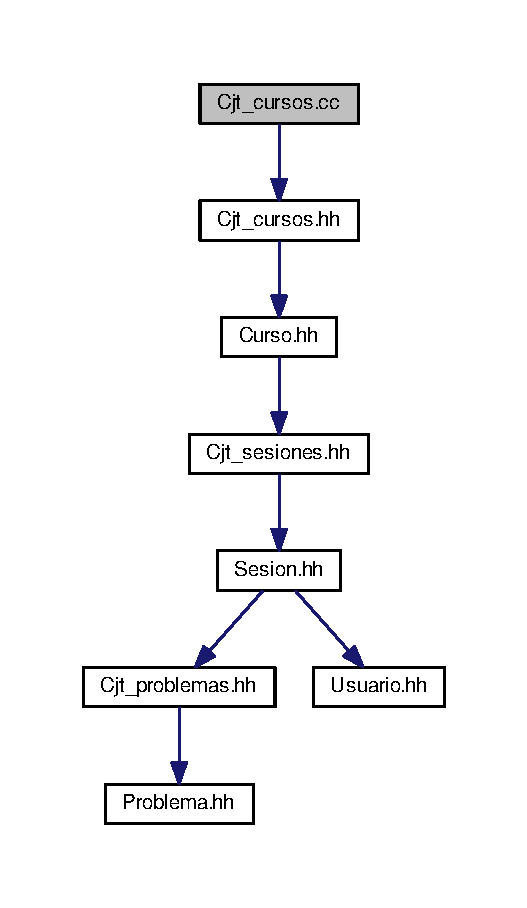
\includegraphics[width=253pt]{_cjt__cursos_8cc__incl}
\end{center}
\end{figure}

\hypertarget{_cjt__cursos_8hh}{}\section{Referencia del Archivo Cjt\+\_\+cursos.\+hh}
\label{_cjt__cursos_8hh}\index{Cjt\+\_\+cursos.\+hh@{Cjt\+\_\+cursos.\+hh}}


Especificación de la clase \mbox{\hyperlink{class_cjt__cursos}{Cjt\+\_\+cursos}} (conjunto de cursos)  


Dependencia gráfica adjunta para Cjt\+\_\+cursos.\+hh\+:
\nopagebreak
\begin{figure}[H]
\begin{center}
\leavevmode
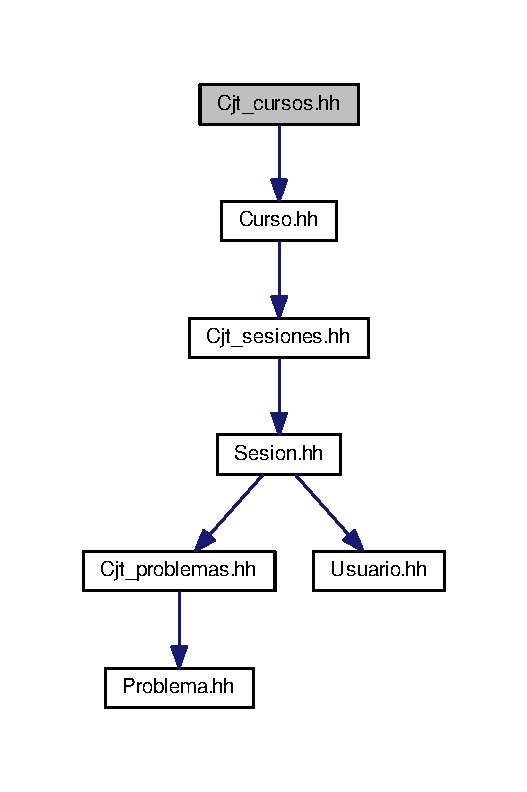
\includegraphics[width=253pt]{_cjt__cursos_8hh__incl}
\end{center}
\end{figure}
\subsection*{Clases}
\begin{DoxyCompactItemize}
\item 
class \mbox{\hyperlink{class_cjt__cursos}{Cjt\+\_\+cursos}}
\begin{DoxyCompactList}\small\item\em Representa un \mbox{\hyperlink{class_cjt__cursos}{Cjt\+\_\+cursos}} (conjunto de cursos) \end{DoxyCompactList}\end{DoxyCompactItemize}


\subsection{Descripción detallada}
Especificación de la clase \mbox{\hyperlink{class_cjt__cursos}{Cjt\+\_\+cursos}} (conjunto de cursos) 


\hypertarget{_cjt__problemas_8cc}{}\section{Referencia del Archivo Cjt\+\_\+problemas.\+cc}
\label{_cjt__problemas_8cc}\index{Cjt\+\_\+problemas.\+cc@{Cjt\+\_\+problemas.\+cc}}
Dependencia gráfica adjunta para Cjt\+\_\+problemas.\+cc\+:
\nopagebreak
\begin{figure}[H]
\begin{center}
\leavevmode
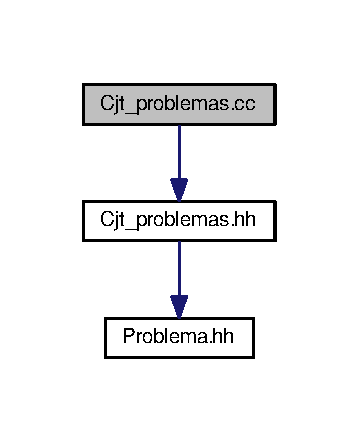
\includegraphics[width=172pt]{_cjt__problemas_8cc__incl}
\end{center}
\end{figure}

\hypertarget{_cjt__problemas_8hh}{}\section{Referencia del Archivo Cjt\+\_\+problemas.\+hh}
\label{_cjt__problemas_8hh}\index{Cjt\+\_\+problemas.\+hh@{Cjt\+\_\+problemas.\+hh}}


Especificación de la clase \mbox{\hyperlink{class_cjt__problemas}{Cjt\+\_\+problemas}} (conjunto de problemas)  


Dependencia gráfica adjunta para Cjt\+\_\+problemas.\+hh\+:
\nopagebreak
\begin{figure}[H]
\begin{center}
\leavevmode
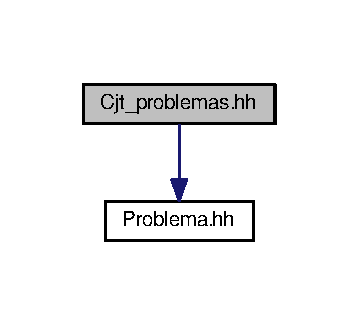
\includegraphics[width=172pt]{_cjt__problemas_8hh__incl}
\end{center}
\end{figure}
\subsection*{Clases}
\begin{DoxyCompactItemize}
\item 
class \mbox{\hyperlink{class_cjt__problemas}{Cjt\+\_\+problemas}}
\begin{DoxyCompactList}\small\item\em Representa un \mbox{\hyperlink{class_cjt__problemas}{Cjt\+\_\+problemas}} (conjunto de problemas) \end{DoxyCompactList}\item 
struct \mbox{\hyperlink{struct_cjt__problemas_1_1prat}{Cjt\+\_\+problemas\+::prat}}
\end{DoxyCompactItemize}


\subsection{Descripción detallada}
Especificación de la clase \mbox{\hyperlink{class_cjt__problemas}{Cjt\+\_\+problemas}} (conjunto de problemas) 


\hypertarget{_cjt__sesiones_8cc}{}\section{Referencia del Archivo Cjt\+\_\+sesiones.\+cc}
\label{_cjt__sesiones_8cc}\index{Cjt\+\_\+sesiones.\+cc@{Cjt\+\_\+sesiones.\+cc}}
Dependencia gráfica adjunta para Cjt\+\_\+sesiones.\+cc\+:
\nopagebreak
\begin{figure}[H]
\begin{center}
\leavevmode
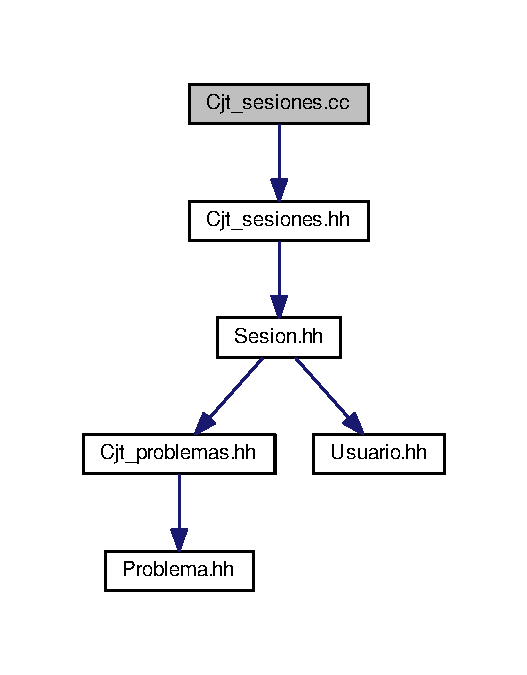
\includegraphics[width=253pt]{_cjt__sesiones_8cc__incl}
\end{center}
\end{figure}

\hypertarget{_cjt__sesiones_8hh}{}\section{Referencia del Archivo Cjt\+\_\+sesiones.\+hh}
\label{_cjt__sesiones_8hh}\index{Cjt\+\_\+sesiones.\+hh@{Cjt\+\_\+sesiones.\+hh}}


Especificación de la clase conjunto de sesiones.  


Dependencia gráfica adjunta para Cjt\+\_\+sesiones.\+hh\+:
\nopagebreak
\begin{figure}[H]
\begin{center}
\leavevmode
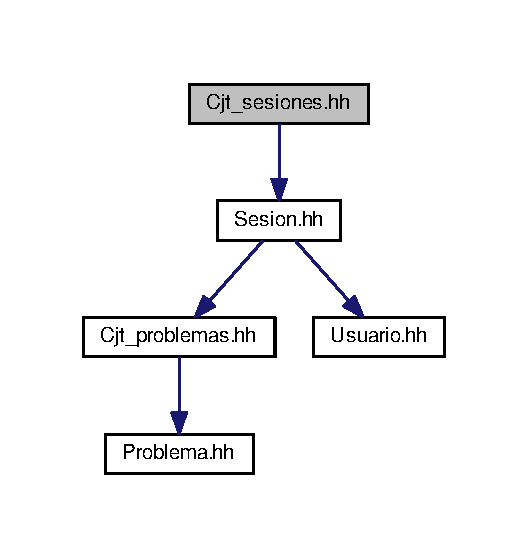
\includegraphics[width=253pt]{_cjt__sesiones_8hh__incl}
\end{center}
\end{figure}
\subsection*{Clases}
\begin{DoxyCompactItemize}
\item 
class \mbox{\hyperlink{class_cjt__sesiones}{Cjt\+\_\+sesiones}}
\begin{DoxyCompactList}\small\item\em Representa un \mbox{\hyperlink{class_cjt__sesiones}{Cjt\+\_\+sesiones}} (conjunto de sesiones) \end{DoxyCompactList}\end{DoxyCompactItemize}


\subsection{Descripción detallada}
Especificación de la clase conjunto de sesiones. 


\hypertarget{_cjt__usuarios_8cc}{}\section{Referencia del Archivo Cjt\+\_\+usuarios.\+cc}
\label{_cjt__usuarios_8cc}\index{Cjt\+\_\+usuarios.\+cc@{Cjt\+\_\+usuarios.\+cc}}
Dependencia gráfica adjunta para Cjt\+\_\+usuarios.\+cc\+:
\nopagebreak
\begin{figure}[H]
\begin{center}
\leavevmode
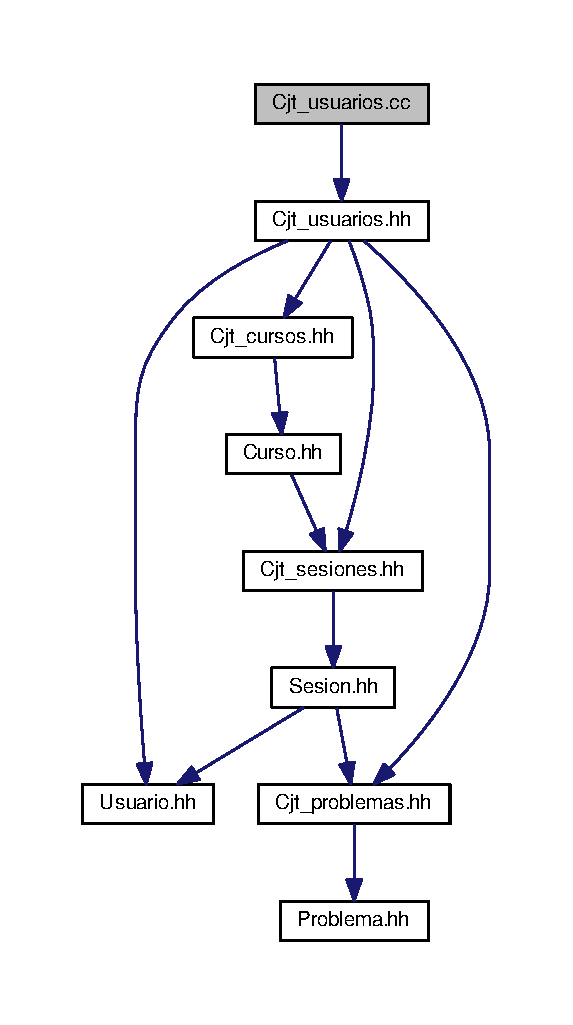
\includegraphics[width=275pt]{_cjt__usuarios_8cc__incl}
\end{center}
\end{figure}

\hypertarget{_cjt__usuarios_8hh}{}\section{Referencia del Archivo Cjt\+\_\+usuarios.\+hh}
\label{_cjt__usuarios_8hh}\index{Cjt\+\_\+usuarios.\+hh@{Cjt\+\_\+usuarios.\+hh}}


Especificación de la clase \mbox{\hyperlink{class_cjt__usuarios}{Cjt\+\_\+usuarios}} (conjunto de usuarios)  


Dependencia gráfica adjunta para Cjt\+\_\+usuarios.\+hh\+:
\nopagebreak
\begin{figure}[H]
\begin{center}
\leavevmode
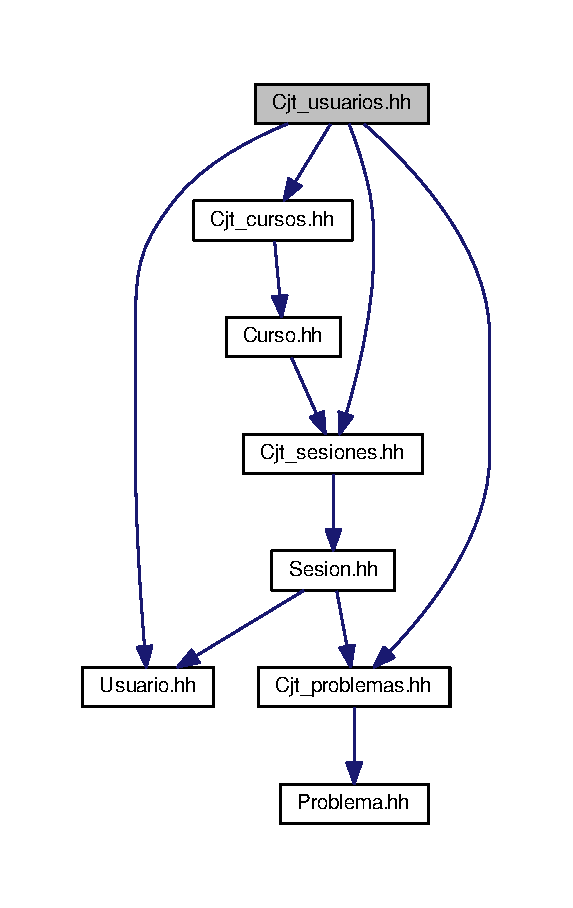
\includegraphics[width=275pt]{_cjt__usuarios_8hh__incl}
\end{center}
\end{figure}
\subsection*{Clases}
\begin{DoxyCompactItemize}
\item 
class \mbox{\hyperlink{class_cjt__usuarios}{Cjt\+\_\+usuarios}}
\begin{DoxyCompactList}\small\item\em Representa un \mbox{\hyperlink{class_cjt__usuarios}{Cjt\+\_\+usuarios}} (conjunto de usuarios) \end{DoxyCompactList}\end{DoxyCompactItemize}


\subsection{Descripción detallada}
Especificación de la clase \mbox{\hyperlink{class_cjt__usuarios}{Cjt\+\_\+usuarios}} (conjunto de usuarios) 


\hypertarget{_curso_8cc}{}\section{Referencia del Archivo Curso.\+cc}
\label{_curso_8cc}\index{Curso.\+cc@{Curso.\+cc}}
Dependencia gráfica adjunta para Curso.\+cc\+:
\nopagebreak
\begin{figure}[H]
\begin{center}
\leavevmode
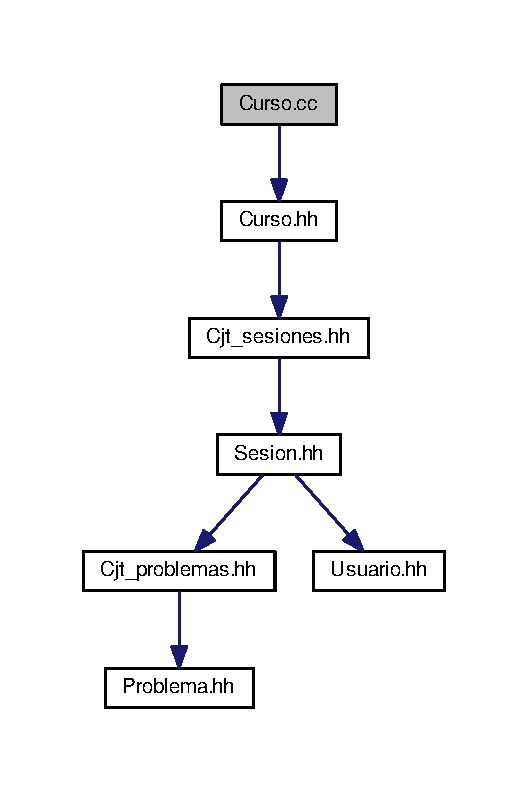
\includegraphics[width=253pt]{_curso_8cc__incl}
\end{center}
\end{figure}

\hypertarget{_curso_8hh}{}\section{Referencia del Archivo Curso.\+hh}
\label{_curso_8hh}\index{Curso.\+hh@{Curso.\+hh}}


Especificación de la clase \mbox{\hyperlink{class_curso}{Curso}}.  


Dependencia gráfica adjunta para Curso.\+hh\+:
\nopagebreak
\begin{figure}[H]
\begin{center}
\leavevmode
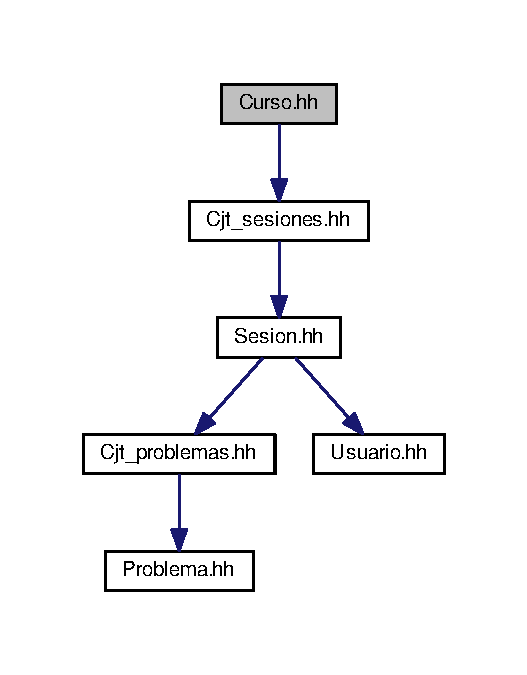
\includegraphics[width=253pt]{_curso_8hh__incl}
\end{center}
\end{figure}
\subsection*{Clases}
\begin{DoxyCompactItemize}
\item 
class \mbox{\hyperlink{class_curso}{Curso}}
\begin{DoxyCompactList}\small\item\em Representa un \mbox{\hyperlink{class_curso}{Curso}} de la plataforma. \end{DoxyCompactList}\end{DoxyCompactItemize}


\subsection{Descripción detallada}
Especificación de la clase \mbox{\hyperlink{class_curso}{Curso}}. 

Un curso está formado por el número de inscritos, el número de usuarios que lo han completado (graduados), los identificadores de las sesiones y todos sus problemas con la sesion en la que pertenece cada uno. 
\hypertarget{_problema_8cc}{}\section{Referencia del Archivo Problema.\+cc}
\label{_problema_8cc}\index{Problema.\+cc@{Problema.\+cc}}
Dependencia gráfica adjunta para Problema.\+cc\+:
\nopagebreak
\begin{figure}[H]
\begin{center}
\leavevmode
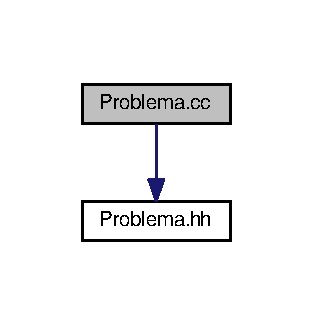
\includegraphics[width=150pt]{_problema_8cc__incl}
\end{center}
\end{figure}

\hypertarget{_problema_8hh}{}\section{Referencia del Archivo Problema.\+hh}
\label{_problema_8hh}\index{Problema.\+hh@{Problema.\+hh}}


Especificación de la clase \mbox{\hyperlink{class_problema}{Problema}}.  


\subsection*{Clases}
\begin{DoxyCompactItemize}
\item 
class \mbox{\hyperlink{class_problema}{Problema}}
\begin{DoxyCompactList}\small\item\em Representa un \mbox{\hyperlink{class_problema}{Problema}} de una \mbox{\hyperlink{class_sesion}{Sesion}} de la plataforma. \end{DoxyCompactList}\end{DoxyCompactItemize}


\subsection{Descripción detallada}
Especificación de la clase \mbox{\hyperlink{class_problema}{Problema}}. 

Un problema forma parte de una sesion. Este está formado por el número de envios totales que se han realizado y el número de envios correctos. 
\hypertarget{program_8cc}{}\section{Referencia del Archivo program.\+cc}
\label{program_8cc}\index{program.\+cc@{program.\+cc}}
Dependencia gráfica adjunta para program.\+cc\+:
\nopagebreak
\begin{figure}[H]
\begin{center}
\leavevmode
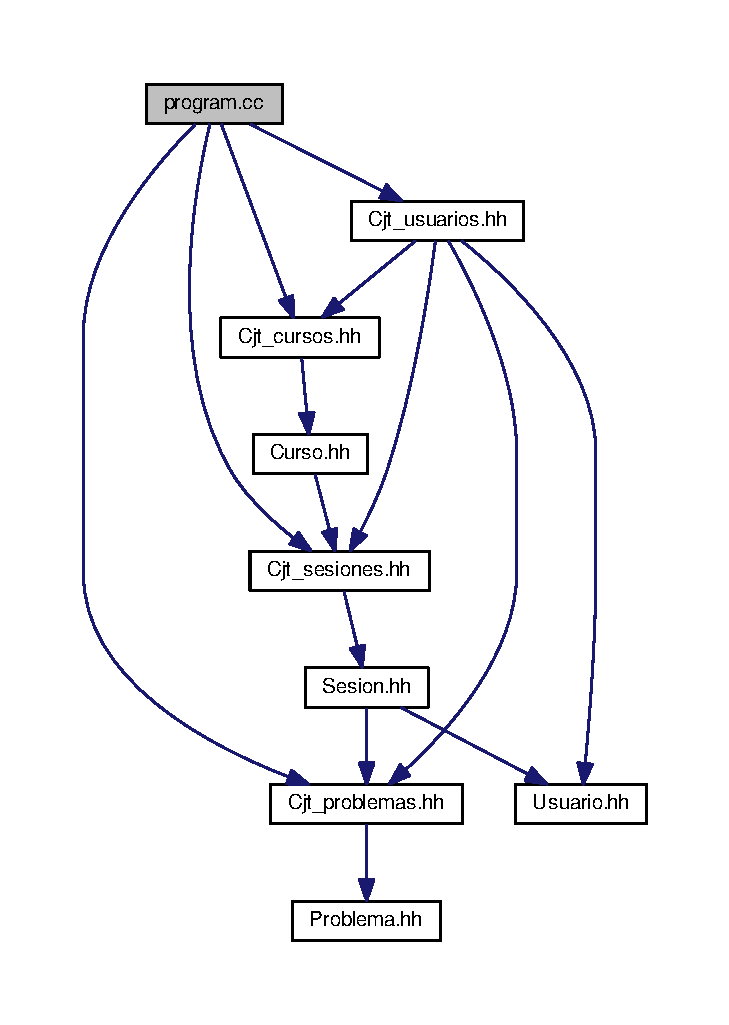
\includegraphics[width=350pt]{program_8cc__incl}
\end{center}
\end{figure}
\subsection*{Funciones}
\begin{DoxyCompactItemize}
\item 
int \mbox{\hyperlink{program_8cc_ae66f6b31b5ad750f1fe042a706a4e3d4}{main}} ()
\end{DoxyCompactItemize}


\subsection{Documentación de las funciones}
\mbox{\Hypertarget{program_8cc_ae66f6b31b5ad750f1fe042a706a4e3d4}\label{program_8cc_ae66f6b31b5ad750f1fe042a706a4e3d4}} 
\index{program.\+cc@{program.\+cc}!main@{main}}
\index{main@{main}!program.\+cc@{program.\+cc}}
\subsubsection{\texorpdfstring{main()}{main()}}
{\footnotesize\ttfamily int main (\begin{DoxyParamCaption}{ }\end{DoxyParamCaption})}



Definición en la línea 34 del archivo program.\+cc.


\begin{DoxyCode}
34            \{
35   \mbox{\hyperlink{class_cjt__problemas}{Cjt\_problemas}} problems;
36   problems.\mbox{\hyperlink{class_cjt__problemas_a38d418d08be011f8cfbdfdac1ad2451a}{leer\_problemas}}(); \textcolor{comment}{//lectuda inicial de problemas}
37   \mbox{\hyperlink{class_cjt__sesiones}{Cjt\_sesiones}} sesiones;
38   sesiones.\mbox{\hyperlink{class_cjt__sesiones_ac550e55acf1c249058d274214ba8f655}{leer\_sesiones}}(); \textcolor{comment}{//lectura inicial de sesiones}
39   \mbox{\hyperlink{class_cjt__cursos}{Cjt\_cursos}} cursos;
40   cursos.\mbox{\hyperlink{class_cjt__cursos_a71a9a083e2abceee34329462a804637a}{leer\_cursos}}(sesiones); \textcolor{comment}{//lectura inicial de cursos}
41   \mbox{\hyperlink{class_cjt__usuarios}{Cjt\_usuarios}} users;
42   users.\mbox{\hyperlink{class_cjt__usuarios_aeb27ae7d46e9b78e2d477df74461bc68}{leer\_usuarios}}(); \textcolor{comment}{//lectura inicial de usuarios}
43 
44   \textcolor{keywordtype}{int} c; \textcolor{comment}{//IDENTIFICADOR Curso}
45   \textcolor{keywordtype}{string} p, s, u; \textcolor{comment}{//IDENTIFICADORES Problema, Sesion y Usuario respectivamente}
46 
47   \textcolor{keywordtype}{string} op; \textcolor{comment}{//CODIGO DE OPERACIÓN}
48   \textcolor{keywordflow}{while} (cin >> op and op != \textcolor{stringliteral}{"fin"}) \{
49 
50     \textcolor{comment}{//1- nuevo\_problema}
51     \textcolor{keywordflow}{if} (op == \textcolor{stringliteral}{"np"} or op == \textcolor{stringliteral}{"nuevo\_problema"})\{
52       cin >> p;
53       cout << \textcolor{stringliteral}{"#"} << op << \textcolor{stringliteral}{" "} << p << endl;
54       problems.\mbox{\hyperlink{class_cjt__problemas_a6c84adcab542d776e02f851eb9d3da82}{nuevo\_problema}}(p);
55     \}
56 
57     \textcolor{comment}{//2- nueva\_sesion}
58     \textcolor{keywordflow}{else} \textcolor{keywordflow}{if} (op == \textcolor{stringliteral}{"ns"} or op == \textcolor{stringliteral}{"nueva\_sesion"})\{
59       cin >> s;
60       cout << \textcolor{stringliteral}{"#"} << op << \textcolor{stringliteral}{" "} << s << endl;
61       sesiones.\mbox{\hyperlink{class_cjt__sesiones_a7436186b6a6b34354ab5303f6b8bcfa9}{nueva\_sesion}}(s);
62     \}
63 
64     \textcolor{comment}{//3- nuevo\_curso}
65     \textcolor{keywordflow}{else} \textcolor{keywordflow}{if} (op == \textcolor{stringliteral}{"nc"} or op == \textcolor{stringliteral}{"nuevo\_curso"})\{
66       cout << \textcolor{stringliteral}{"#"} << op << endl;
67       cursos.\mbox{\hyperlink{class_cjt__cursos_ae2e0a96f014dda94b0d8465838cf14b6}{nuevo\_curso}}(sesiones);
68     \}
69 
70     \textcolor{comment}{//4- alta\_usuario}
71     \textcolor{keywordflow}{else} \textcolor{keywordflow}{if} (op == \textcolor{stringliteral}{"a"} or op == \textcolor{stringliteral}{"alta\_usuario"})\{
72       cin >> u;
73       cout << \textcolor{stringliteral}{"#"} << op << \textcolor{stringliteral}{" "} << u << endl;
74       users.\mbox{\hyperlink{class_cjt__usuarios_af2bc90f54125530ce07dde609dfbe43b}{alta\_usuario}}(u);
75     \}
76 
77     \textcolor{comment}{//5- baja\_usuario}
78     \textcolor{keywordflow}{else} \textcolor{keywordflow}{if} (op == \textcolor{stringliteral}{"b"} or op == \textcolor{stringliteral}{"baja\_usuario"})\{
79       cin >> u;
80       cout << \textcolor{stringliteral}{"#"} << op << \textcolor{stringliteral}{" "} << u << endl;
81       users.\mbox{\hyperlink{class_cjt__usuarios_a318dcc3682784e73e0fe98ddbf39350c}{baja\_usuario}}(u, cursos);
82     \}
83 
84     \textcolor{comment}{//6- inscribir\_curso}
85     \textcolor{keywordflow}{else} \textcolor{keywordflow}{if} (op == \textcolor{stringliteral}{"i"} or op == \textcolor{stringliteral}{"inscribir\_curso"})\{
86       cin >> u >> c;
87       cout << \textcolor{stringliteral}{"#"} << op << \textcolor{stringliteral}{" "} << u << \textcolor{stringliteral}{" "} << c << endl;
88       users.\mbox{\hyperlink{class_cjt__usuarios_a94946c0533b04337bee7395f1dac0366}{inscribir\_curso}}(u, c, cursos, sesiones);
89     \}
90 
91     \textcolor{comment}{// 7- curso\_usuario}
92     \textcolor{keywordflow}{else} \textcolor{keywordflow}{if} (op == \textcolor{stringliteral}{"cu"} or op == \textcolor{stringliteral}{"curso\_usuario"})\{
93       cin >> u;
94       cout << \textcolor{stringliteral}{"#"} << op << \textcolor{stringliteral}{" "} << u << endl;
95       users.\mbox{\hyperlink{class_cjt__usuarios_a0a29517de316ac00a23f26df00ef779b}{curso\_usuario}}(u);
96     \}
97 
98     \textcolor{comment}{//8- sesion\_problema}
99     \textcolor{keywordflow}{else} \textcolor{keywordflow}{if} (op == \textcolor{stringliteral}{"sp"} or op == \textcolor{stringliteral}{"sesion\_problema"})\{
100       cin >> c >> p;
101       cout << \textcolor{stringliteral}{"#"} << op << \textcolor{stringliteral}{" "} << c << \textcolor{stringliteral}{" "} << p << endl;
102       \textcolor{keywordflow}{if} (problems.\mbox{\hyperlink{class_cjt__problemas_a90b230192705dd6f2e15fb10514a5814}{existe\_problema}}(p)) \{
103         \textcolor{keywordflow}{if} (cursos.\mbox{\hyperlink{class_cjt__cursos_aed873ef8285d1f33c391bd4d808185de}{existe\_curso}}(c)) \{
104           \textcolor{keywordflow}{if} (cursos.\mbox{\hyperlink{class_cjt__cursos_a7b2a3da42d49f10bd6413fa00dbe9012}{existe\_problema}}(p, c)) \{
105             cout << cursos.\mbox{\hyperlink{class_cjt__cursos_acc9074c9338d31947bdd84e3498580be}{sesion\_problema}}(c, p) << endl;
106           \}
107           \textcolor{keywordflow}{else} cout << \textcolor{stringliteral}{"error: el problema no pertenece al curso"} << endl;
108         \}
109         \textcolor{keywordflow}{else} cout << \textcolor{stringliteral}{"error: el curso no existe"} << endl;
110       \}
111       \textcolor{keywordflow}{else} cout << \textcolor{stringliteral}{"error: el problema no existe"} << endl;
112     \}
113 
114     \textcolor{comment}{//9- problemas\_resueltos}
115     \textcolor{keywordflow}{else} \textcolor{keywordflow}{if} (op == \textcolor{stringliteral}{"pr"} or op == \textcolor{stringliteral}{"problemas\_resueltos"})\{
116       cin >> u;
117       cout << \textcolor{stringliteral}{"#"} << op << \textcolor{stringliteral}{" "} << u << endl;
118       users.\mbox{\hyperlink{class_cjt__usuarios_a08ce8035512646dec31f4959dc8aa891}{problemas\_resueltos}}(u);
119     \}
120 
121     \textcolor{comment}{//10- problemas\_enviables}
122     \textcolor{keywordflow}{else} \textcolor{keywordflow}{if} (op == \textcolor{stringliteral}{"pe"} or op == \textcolor{stringliteral}{"problemas\_enviables"})\{
123       cin >> u;
124       cout << \textcolor{stringliteral}{"#"} << op << \textcolor{stringliteral}{" "} << u << endl;
125       users.\mbox{\hyperlink{class_cjt__usuarios_a60b4396cdd65a2aa4b7a8706dabbe08b}{problemas\_enviables}}(u);
126     \}
127     
128     \textcolor{comment}{//11- envio}
129     \textcolor{keywordflow}{else} \textcolor{keywordflow}{if} (op == \textcolor{stringliteral}{"e"} or op == \textcolor{stringliteral}{"envio"})\{
130       \textcolor{keywordtype}{int} nota;
131       cin >> u >> p >> nota;
132       \textcolor{keywordtype}{bool} r = \textcolor{keyword}{true};
133       \textcolor{keywordflow}{if} (nota == 0) r = \textcolor{keyword}{false};
134       cout << \textcolor{stringliteral}{"#"} << op << \textcolor{stringliteral}{" "} << u << \textcolor{stringliteral}{" "} << p << \textcolor{stringliteral}{" "} << nota << endl;
135       users.\mbox{\hyperlink{class_cjt__usuarios_ac4e3616bd8af5d118d4039d203805e76}{envio}}(u, p, r, problems, sesiones, cursos);
136     \}
137     
138     \textcolor{comment}{//12- listar\_problemas}
139     \textcolor{keywordflow}{else} \textcolor{keywordflow}{if} (op == \textcolor{stringliteral}{"lp"} or op == \textcolor{stringliteral}{"listar\_problemas"})\{
140       cout << \textcolor{stringliteral}{"#"} << op << endl;
141       problems.\mbox{\hyperlink{class_cjt__problemas_a4cc09ed948f0315d5257d0d3a11e4dd5}{listar\_problemas}}();
142     \}
143 
144     \textcolor{comment}{//escribir\_problema}
145     \textcolor{keywordflow}{else} \textcolor{keywordflow}{if} (op == \textcolor{stringliteral}{"ep"} or op == \textcolor{stringliteral}{"escribir\_problema"})\{
146       cin >> p;
147       cout << \textcolor{stringliteral}{"#"} << op << \textcolor{stringliteral}{" "} << p << endl;
148       problems.\mbox{\hyperlink{class_cjt__problemas_a4fbbf5935069783a5ced92c5b169c330}{escribir\_problema}}(p);
149     \}
150 
151     \textcolor{comment}{//13- listar\_sesiones}
152     \textcolor{keywordflow}{else} \textcolor{keywordflow}{if} (op == \textcolor{stringliteral}{"ls"} or op == \textcolor{stringliteral}{"listar\_sesiones"})\{
153       cout << \textcolor{stringliteral}{"#"} << op << endl;
154       sesiones.\mbox{\hyperlink{class_cjt__sesiones_a58e65694f1e4b544ae3c3e85cf329eeb}{listar\_sesiones}}();
155     \}
156 
157     \textcolor{comment}{//escribir\_sesion}
158     \textcolor{keywordflow}{else} \textcolor{keywordflow}{if} (op == \textcolor{stringliteral}{"es"} or op == \textcolor{stringliteral}{"escribir\_sesion"})\{
159       cin >> s;
160       cout << \textcolor{stringliteral}{"#"} << op << \textcolor{stringliteral}{" "} << s << endl;
161       sesiones.\mbox{\hyperlink{class_cjt__sesiones_ab3d1427eaac58e65fa341d60f9e2a3b3}{escribir\_sesion}}(s);
162     \}
163 
164     \textcolor{comment}{//14- listar\_cursos}
165     \textcolor{keywordflow}{else} \textcolor{keywordflow}{if} (op == \textcolor{stringliteral}{"lc"} or op == \textcolor{stringliteral}{"listar\_cursos"})\{
166       cout << \textcolor{stringliteral}{"#"} << op << endl;
167       cursos.\mbox{\hyperlink{class_cjt__cursos_abba27f9593cae77bf02909a06454ec43}{listar\_cursos}}();
168     \}
169 
170     \textcolor{comment}{//escribir\_curso}
171     \textcolor{keywordflow}{else} \textcolor{keywordflow}{if} (op == \textcolor{stringliteral}{"ec"} or op == \textcolor{stringliteral}{"escribir\_curso"})\{
172       cin >> c;
173       cout << \textcolor{stringliteral}{"#"} << op << \textcolor{stringliteral}{" "} << c << endl;
174       cursos.\mbox{\hyperlink{class_cjt__cursos_a6c98d2f0a31253b84dc8b4a0ea48c348}{escribir\_curso}}(c);
175     \}
176 
177     \textcolor{comment}{//15- listar\_usuarios}
178     \textcolor{keywordflow}{else} \textcolor{keywordflow}{if} (op == \textcolor{stringliteral}{"lu"} or op == \textcolor{stringliteral}{"listar\_usuarios"})\{
179       cout << \textcolor{stringliteral}{"#"} << op << endl;
180       users.\mbox{\hyperlink{class_cjt__usuarios_adb9a7441da7fb87a524142aaf6e61853}{listar\_usuarios}}();
181     \}
182 
183     \textcolor{comment}{//escribir\_usuario}
184     \textcolor{keywordflow}{else} \textcolor{keywordflow}{if} (op == \textcolor{stringliteral}{"eu"} or op == \textcolor{stringliteral}{"escribir\_usuario"})\{
185       cin >> u;
186       cout << \textcolor{stringliteral}{"#"} << op << \textcolor{stringliteral}{" "} << u << endl;
187       users.\mbox{\hyperlink{class_cjt__usuarios_abf4abc6a1349c504bd0628cfe665df39}{escribir\_usuario}}(u);
188     \}
189   \}
190 \}
\end{DoxyCode}

\hypertarget{_sesion_8cc}{}\section{Referencia del Archivo Sesion.\+cc}
\label{_sesion_8cc}\index{Sesion.\+cc@{Sesion.\+cc}}
Dependencia gráfica adjunta para Sesion.\+cc\+:
\nopagebreak
\begin{figure}[H]
\begin{center}
\leavevmode
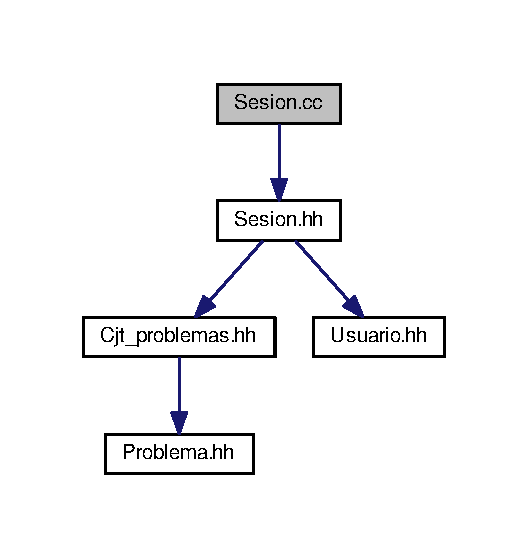
\includegraphics[width=253pt]{_sesion_8cc__incl}
\end{center}
\end{figure}

\hypertarget{_sesion_8hh}{}\section{Referencia del Archivo Sesion.\+hh}
\label{_sesion_8hh}\index{Sesion.\+hh@{Sesion.\+hh}}


Especificación de la clase sesion.  


Dependencia gráfica adjunta para Sesion.\+hh\+:
\nopagebreak
\begin{figure}[H]
\begin{center}
\leavevmode
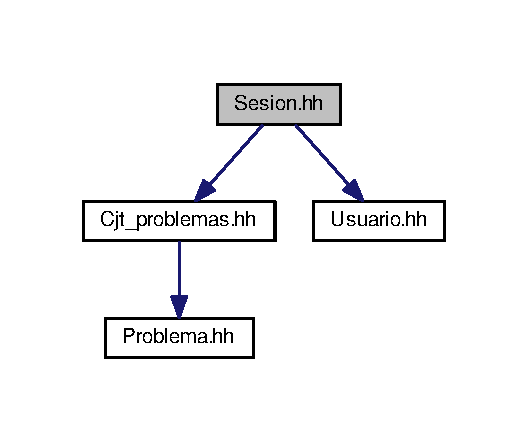
\includegraphics[width=253pt]{_sesion_8hh__incl}
\end{center}
\end{figure}
\subsection*{Clases}
\begin{DoxyCompactItemize}
\item 
class \mbox{\hyperlink{class_sesion}{Sesion}}
\begin{DoxyCompactList}\small\item\em Representa una \mbox{\hyperlink{class_sesion}{Sesion}} de la plataforma. \end{DoxyCompactList}\end{DoxyCompactItemize}


\subsection{Descripción detallada}
Especificación de la clase sesion. 


\hypertarget{_usuario_8cc}{}\section{Referencia del Archivo Usuario.\+cc}
\label{_usuario_8cc}\index{Usuario.\+cc@{Usuario.\+cc}}
Dependencia gráfica adjunta para Usuario.\+cc\+:
\nopagebreak
\begin{figure}[H]
\begin{center}
\leavevmode
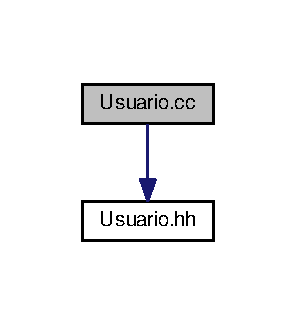
\includegraphics[width=142pt]{_usuario_8cc__incl}
\end{center}
\end{figure}

\hypertarget{_usuario_8hh}{}\section{Referencia del Archivo Usuario.\+hh}
\label{_usuario_8hh}\index{Usuario.\+hh@{Usuario.\+hh}}


Especificación de la clase usuario.  


\subsection*{Clases}
\begin{DoxyCompactItemize}
\item 
class \mbox{\hyperlink{class_usuario}{Usuario}}
\begin{DoxyCompactList}\small\item\em Representa un \mbox{\hyperlink{class_usuario}{Usuario}} registrado en la plataforma. \end{DoxyCompactList}\end{DoxyCompactItemize}


\subsection{Descripción detallada}
Especificación de la clase usuario. 


%--- End generated contents ---

% Index
\backmatter
\newpage
\phantomsection
\clearemptydoublepage
\addcontentsline{toc}{chapter}{Índice}
\printindex

\end{document}
